\documentclass{jpp}

\usepackage{graphicx}
\usepackage{amsmath}
\usepackage{array}
\usepackage{tabularx}
\usepackage{amssymb}
\usepackage{xcolor}
\usepackage{tikz}
\usetikzlibrary{patterns,patterns.meta,decorations.pathreplacing}
\usepackage[normalem]{ulem}
\usepackage{placeins}

\setcounter{topnumber}{3}
\setcounter{totalnumber}{4}
\renewcommand{\topfraction}{0.9}
\renewcommand{\textfraction}{0.07}
\renewcommand{\floatpagefraction}{0.8}

\interfootnotelinepenalty=10000

\setlength{\paperwidth}{174mm}
\setlength{\paperheight}{247mm}
\usepackage[colorlinks=true,
            linkcolor=blue!60!black,
            citecolor=blue!60!black,
            urlcolor=blue!60!black,
            setpagesize=false,
            hypertexnames=false]{hyperref}

\usepackage{cleveref}
\crefformat{section}{\S#2#1#3}
\crefformat{subsection}{\S#2#1#3}
\crefformat{subsubsection}{\S#2#1#3}
\crefformat{figure}{figure~#2#1#3}
\crefformat{equation}{(#2#1#3)}
\crefrangeformat{equation}{(#3#1#4)--(#5#2#6)}
\crefrangeformat{figure}{figures #3#1#4--#5#2#6}
\def\closesymbol{\!}
\newcommand{\order}[1]{O\left(#1\right)}
\newcommand{\orderinline}[1]{O(#1)}
\newcommand{\rmd}{\text{d}}

\newcommand{\bv}{\mathbf{v}}
\newcommand{\br}{\mathbf{r}}
\newcommand{\bB}{\mathbf{B}}

\ifdefined\closesymbol
	\relax
\else
	\def\closesymbol{\relax}
\fi

\newcommand{\pt}{\partial_t}
\newcommand{\px}{\partial_x}
\newcommand{\py}{\partial_y}
\newcommand{\pz}{\partial_z}

\ifdefined\partd
	\renewcommand{\partd}[3][]{\frac{{\partial^{#1} #2}}{{\partial #3}^{#1}}}
\else
	\newcommand{\partd}[3][]{\frac{{\partial^{#1} #2}}{{\partial #3}^{#1}}}
\fi

\ifdefined\vec
	\renewcommand{\vec}[1]{\boldsymbol{#1}}
\else
	\newcommand{\vec}[1]{\boldsymbol{#1}}
\fi

\newcommand{\uvec}[1]{\hat{\boldsymbol{#1}}}
\providecommand{\bcdot}{\vec{\cdot}}

\newcommand{\grad}{{\vec{\nabla}}}
\ifdefined\div
	\renewcommand{\div}{{\grad\bcdot}}
\else
	\newcommand{\div}{{\grad\bcdot}}
\fi

\ifdefined\vr
	\renewcommand{\vr}{{\vec{r}}}
\else
	\newcommand{\vr}{{\vec{r}}}
\fi
\newcommand{\vp}{{\vec{p}}}
\newcommand{\vq}{{\vec{q}}}
\newcommand{\vk}{{\vec{k}}}

\ifdefined\vv
	\renewcommand{\vv}{{\vec{v}}}
\else
	\newcommand{\vv}{{\vec{v}}}
\fi

\newcommand{\vkperp}{{\vk_\perp}}
\newcommand{\kperp}{k_\perp}
\newcommand{\kpar}{k_\parallel}
\newcommand{\vperp}{v_\perp}
\newcommand{\vvperp}{\vv_\perp}
\newcommand{\vpar}{v_\parallel}
\newcommand{\hvpar}{\hat v_\parallel}

\newcommand{\intr}[1][3]{{\int \rmd^{#1} \vec{r} \ }}
\newcommand{\intR}[1][3]{{\int \rmd^{#1} \vec{R} \ }}
\newcommand{\intv}[1][3]{{\int \rmd^{#1} \vec{v} \ }}
\newcommand{\intw}[1][3]{{\int \rmd^{#1} \vec{w} \ }}

\newcommand{\s}{s}
\newcommand{\vth}{v_\text{th}}
\newcommand{\vths}{v_{\text{th}\s}}
\newcommand{\vthi}{v_{\text{th}i}}
\newcommand{\vthe}{v_{\text{th}e}}
\newcommand{\mfp}{\lambda_\text{mfp}}
\newcommand{\ope}{\omega_{\text{p}e}}
\newcommand{\lDe}{\lambda_{\text{D}e}}
\newcommand{\rhoi}{\rho_i}
\newcommand{\rhoe}{\rho_e}
\newcommand{\rhos}{\rho_s}

\newcommand{\fs}{f_{\s}}
\newcommand{\fos}{f_{0\s}}
\newcommand{\Fs}{F_{\s}}
\newcommand{\Fos}{F_{0\s}}
\newcommand{\dfs}{\delta \closesymbol f_{\s}}

\newcommand{\fe}{f_{e}}
\newcommand{\foe}{f_{0e}}
\newcommand{\Fe}{F_{e}}
\newcommand{\Foe}{F_{0e}}
\newcommand{\dfe}{\delta \closesymbol f_{e}}

\newcommand{\fion}{f_{i}}
\newcommand{\foi}{f_{0i}}
\newcommand{\Fi}{F_{i}}
\newcommand{\Foi}{F_{0i}}
\newcommand{\dfi}{\delta \closesymbol f_{i}}

\newcommand{\kperprhoisq}{\kperp^2\rhoi^2}
\newcommand{\kperprhoisqq}{\kperp^4\rhoi^4}
\newcommand{\kperprhoesq}{\kperp^2\rhoe^2}
\newcommand{\kperprhoesqq}{\kperp^4\rhoe^4}
\newcommand{\pbra}[2]{\left\lbrace #1, #2 \right\rbrace}
\newcommand{\pbrainline}[2]{\lbrace #1, #2 \rbrace}

\newcommand{\vR}{{\vec{R}}}
\newcommand{\vE}{\vec{E}}
\newcommand{\vB}{\vec{B}}
\newcommand{\exb}{\(\vE\times\vB\)}

\newcommand{\avgR}[1]{\left\langle #1 \right\rangle_\vec{R}}
\newcommand{\avgRs}[1]{\left\langle #1 \right\rangle_{\vec{R}_\s}}
\newcommand{\avgRinline}[1]{\langle #1 \rangle_\vec{R}}
\newcommand{\avgr}[1]{\left\langle #1 \right\rangle_{\vec{r}}}
\newcommand{\avgrinline}[1]{\langle #1 \rangle_\vec{r}}

	
\emergencystretch=3em
\raggedbottom

\newcommand{\lambdaD}{\lambda_D}
\newcommand{\debye}{\lambda_D^2}
\newcommand{\omstar}{\omega_*}
\newcommand{\omd}{\omega_d}
\newcommand{\Zhat}{\hat{Z}}
\newcommand{\lavg}[1]{\langle #1 \rangle_\lambda}
\newcommand{\gene}{\texttt{GENE}}
\newcommand{\circled}[1]{\tikz[baseline=(char.base)]{\node[shape=circle,draw,inner sep=1.2pt,line width=0.4pt] (char) {\footnotesize #1};}}

\shorttitle{Pair-plasma turbulence in closed-field-line geometry}
\shortauthor{D. Kennedy and G.G. Plunk}

\title{Electron--positron plasma turbulence in closed-field-line geometry}

\author{D.~Kennedy$^{1}$\thanks{Email address for correspondence: daniel.kennedy@ukaea.uk}
  \and G.G.~Plunk$^{2}$}

\affiliation{$^{1}$UKAEA (United Kingdom Atomic Energy Authority), Culham Campus, Abingdon, Oxfordshire, OX14 3DB, UK\\
$^{2}$Max-Planck-Institut f\"ur Plasmaphysik, Greifswald, Germany}

\begin{document}

\maketitle

\begin{abstract}
We study the nonlinear saturation of electron--positron (pair) plasma turbulence in simple closed-field-line geometry. Such geometry is relevant to the APEX experiment that will confine dilute pair plasmas in a levitated dipole \citep{Stoneking2020}, as well as simpler systems such as the $Z$-pinch. From a transit-averaged drift-kinetic theory, we show that the nonlinearity conserves two quadratic invariants, the free energy $W$ and the electrostatic energy $E$. Following \citet{Fjortoft1953}, we predict a dual cascade in which $E$ inverse-cascades to perpendicular scales above the Debye length, while $W$ cascades forward to small scales. We further argue that, when the assumption of constant magnetic field strength is relaxed, the forward cascade develops a parallel leg, and that the free energy acquires pitch-angle structure as it does so. We test this theory with nonlinear gyrokinetic simulations. In the $Z$-pinch limit we measure the dual cascade directly. We find that the saturated state is dominated by zonal flows and that the transport flux collapses to a small residual level. At stronger drive the same zonal-locked state also carries large-scale coherent vortices, the real-space signature of the scale-independent interchange. In the dipole, the saturated end state is again zonal-flow-dominated. The inverse cascade drives the electrostatic energy into zonal flows that suppress the fluctuations, and the transport is reduced to a small residual. At strong drive, the residual particle flux is inwards, an up-gradient pinch that would peak the density profile. This bodes well for the magnetic confinement of pair plasmas in closed-field-line geometry.
\end{abstract}

\section{Introduction}\label{sec:intro}
The magnetic confinement of an electron--positron (pair) plasma in the laboratory is within reach. The APEX and EPOS programmes aim to confine dilute pair plasmas in a levitated dipole and a compact stellarator respectively \citep{Pedersen2012, Stoneking2020}. In the APEX experiment, the aim is to produce a (relatively) cold and dilute electron--positron plasma. The two species have equal mass $m$, equilibrium density $n,$ and temperature $T$, and carry charges $q_p = -q_e \equiv e$. The expected density and temperature are such that the system size exceeds the Debye length, and the Debye length exceeds the Larmor radius by roughly three orders of magnitude. In the laboratory regime, the system is well described by gyrokinetic theory \citep{Abel2013} in the ordering \begin{equation} \rho \ll \lambdaD \ll L,\label{eq:ordering} \end{equation} where $\rho \equiv \sqrt{mT}/(eB)$ is the Larmor radius, $\lambdaD \equiv \sqrt{\epsilon_0 T/(2 n_0 e^2)}$ the Debye length (with $\epsilon_0$ the vacuum permittivity), and $L$ the system size, provided the target magnetic field of $B = 1\rm{T}$ is attained. Motivated by APEX, we are therefore interested in plasmas satisfying the strongly magnetised ordering $\rho \ll \lambda_{D}$ as well as the standard gyrokinetic ordering. In such plasmas, electrostatic interchange instabilities are expected to be present at scales similar to $\lambdaD,$ with frequencies much smaller than the transit frequency of the particles \citep{Helander2014}. Unstable drift waves can be absent in such plasmas.

It has been shown by \citet{Helander2014} that pair plasmas are exactly stable to electrostatic drift modes in straight slab geometry, a result also extended to electromagnetic drift modes \citep{HelanderConnor2016}, provided that the temperature and density profiles are identical (``symmetric'' pair plasmas). In a straight slab, this symmetry can be broken by introducing e.g., ion contamination. Once the symmetry is broken, drift instabilities can be excited \citep{Mishchenko2018, KennedyMishchenko2019}. In a sheared slab, pure pair plasmas are also prone to current-driven reconnecting instabilities \citep{Zocco2017} but there are no drift waves. Note that asymmetry between the species is needed also in this case since the ambient electron flow velocity must differ from the positron one for the ambient current to be finite. 

Perfect symmetry can also be broken geometrically when the magnetic field has finite magnetic curvature. Unequal (in sign) curvature drifts mean the plasma can once again be driven unstable by density and temperature gradients, even when the profiles are symmetric. The linear stability of such systems has been explored systematically. The kinetic dispersion relation has been solved in the $Z$-pinch and point-dipole limits \citep{MPH2018}, and these results were verified using linear gyrokinetic simulations, firstly in tokamak and stellarator geometry \citep{Kennedy2018}, and then in the dipole flux tube relevant to the APEX experiment \citep{Kennedy2020}. Recent studies have also explored the strong-field cyclotron-cooling regime \citep{KennedyHelander2021a, KennedyHelander2021} that the APEX experiment is expected to access. The nonlinear stability of point dipole pair plasmas was addressed by \citet{Helander2017}, who bounded the available energy of a confined pair-plasma equilibrium and showed that the turbulent transport it can sustain must be small. Excitingly, \citet{Helander2017} identified, within the region of linear stability, a narrow window in which pair plasmas carry no available energy and so cannot drive turbulence at all. 

\Cref{fig:dipole_stability} summarises the stability landscape for a symmetric electron-positron plasma in a dipole, in the flux-label gradient variables $L_\psi/L_n = |\rmd\ln n/\rmd\ln\psi|$ and $L_\psi/L_T = |\rmd\ln T/\rmd\ln\psi|$ of \citet{HelanderConnor2016}. The figure shows two linear thresholds and the ground-state window they enclose. The experimental effort towards magnetised pair plasmas is reviewed by \citet{Stoneking2020}, and the linear gyrokinetic theory surveyed above is reviewed by \citet{Mishchenko2023}.

\begin{figure}
\centering
\begin{tikzpicture}[x=1.05cm,y=1.05cm,>=latex,font=\small,
                    boxed/.style={inner sep=2pt, fill=white},
                    plain/.style={inner sep=2pt}]

  \fill[pattern=north east lines, pattern color=black]
        (0,0) -- (3,2) -- (0,2) -- cycle;
  \fill[pattern=north west lines, pattern color=black]
        (0,0) -- (3,2) -- (0,2) -- cycle;
  \draw[black,semithick,densely dotted] (0,2) -- (3.3333,2);
  \draw[black,semithick,densely dotted] (0,0) -- (7.0,4.6667);

  \draw[black,thick] (0,6.6667) -- (6.6667,0);

  \draw[black,thick,dashed] (1.3333,0) -- (7.0,5.6667);

  \draw[->] (0,0) -- (7.6,0);
  \draw[->] (0,0) -- (0,7.6);
  \node[plain,below] at (3.8,-0.55) {$L_\psi/L_n$};
  \node[plain,rotate=90,above] at (-0.68,3.8) {$L_\psi/L_T$};
  \foreach \t in {1,2,3,4,5,6,7}{
    \draw (\t,0) -- ++(0,-2.2pt);
    \draw (0,\t) -- ++(-2.2pt,0);
  }
  \foreach \t in {2,4,6}{
    \node[plain,below] at (\t,-0.06) {$\t$};
    \node[plain,left]  at (-0.06,\t) {$\t$};
  }

  \node[boxed,rotate=-45,text=black,font=\small] at (2.35,4.317)
        {$L_\psi/L_n + L_\psi/L_T = 20/3$};
  \node[boxed,rotate=45,text=black,font=\small] at (5.85,4.517)
        {$L_\psi/L_n - L_\psi/L_T = 4/3$};
  \node[plain,anchor=west,text=black,font=\small] at (7.05,4.6667)
        {$\eta = 2/3$};

  \node[plain,align=center,font=\small,text=black] at (3.95,6.30)
        {unstable to\\ interchange modes};
  \node[plain,align=center,font=\small,text=black] at (6.15,2.10)
        {unstable to\\ both};
  \node[plain,align=center,font=\small,text=black] at (3.95,0.50)
        {unstable to low-frequency\\ electrostatic (entropy) modes};
  \node[plain,font=\small,text=black] at (0.72,5.05) {stable};
  \node[plain,text=black,font=\small] (aew) at (1.55,3.25)
        {turbulence-free};
  \draw[black,semithick,->] (aew.south) -- (1.30,1.30);
\end{tikzpicture}
\caption{Linear stability of a symmetric pair plasma in a point dipole, in the flux-label gradient variables of \citet{HelanderConnor2016} (their figure~1; see also figure~2 of \citealt{Stoneking2020}). Solid: the interchange threshold. Dashed: the resonant (low-frequency electrostatic) threshold, the entropy mode \citep{Ricci2006, Kobayashi2009, Hoffmann2023}. Dotted: the ray $\eta = 2/3$, on which the two thresholds meet. Cross-hatched: the ground-state window of \citet{Helander2017}, within which the plasma carries no available energy and can drive no turbulence.}
\label{fig:dipole_stability}
\end{figure}

In this work, we concern ourselves with the nature of electron--positron plasma turbulence in simple closed-field-line geometries (the $Z$-pinch and the dipole) when the plasma is linearly unstable to instabilities at scales similar to the Debye length. The layout of this paper is as follows. In~\cref{sec:theory}, we introduce the nonlinear transit-averaged drift-kinetic equations that describe the evolution of fluctuations driven by long-wavelength interchange-like instabilities. We identify two quadratic invariants of the bounce-averaged drift-kinetic nonlinearity, the free energy $W$ and the electrostatic energy $E$. We then run a Fj\o rtoft argument \citep{Fjortoft1953} to predict a dual cascade: an inverse cascade of $E$ to large perpendicular scales, together with a forward cascade of $W$ through phase space to small scales. We argue that when the assumption of constant magnetic field strength is relaxed, the free energy acquires structure in the full four-dimensional phase space. In~\cref{sec:setup} we test these theoretical predictions in local gyrokinetic simulations using the code \gene\, \citep{Jenko2000}. We first briefly discuss our simulation setup and the linear stability landscape. We find excellent agreement between our linear results and existing analytic theory. In~\cref{sec:nonlinear}, we present nonlinear simulations in $Z$-pinch geometry. We find that the saturated state is strongly self-regulated. In the $Z$-pinch limit the electrostatic energy concentrates in large-scale zonal flows and the turbulent transport collapses to a small residual level. \textcolor{red}{An} inward particle pinch is found above a drive threshold. We identify the dual cascade using spectral flux diagnostics. We generalise to the dipole geometry in~\cref{sec:dipole}. There the dual cascade extends into a four-dimensional phase space. The forward $W$ cascade develops a parallel leg inaccessible to the constant-$|\mathbf{B}|$ $Z$-pinch, and the free energy acquires pitch-angle structure (passing-weighted) as it does so. We present our conclusions in~\cref{sec:conclusions}. In the strongly-driven limit the $Z$-pinch equations close into a two-field fluid model, this model is derived in \cref{app:fluid}. Further details of the numerical setup and benchmarking are provided in \cref{app:dipole_impl}--\cref{app:aspect}.


\section{Theoretical background}\label{sec:theory}
We consider a symmetric electron--positron plasma confined in a closed-field-line magnetic geometry with zero geodesic curvature. We work in the electrostatic, low-$\beta$ limit and adopt magnetic flux coordinates $(\psi, \alpha, l)$, in which $\mathbf{B} = \grad\psi \times \grad\alpha$ and $l$ is the arc length along the field line.

\subsection{From the gyrokinetic equation to the bounce-averaged drift-kinetic equation}\label{sec:gk_to_dke}

Our starting point is the electrostatic $\delta \! f$ gyrokinetic equation for each species $a \in \{e, p\}$ [e.g., \citet{Abel2013}]. The perturbed distribution splits into the adiabatic (Boltzmann) response, evaluated at the particle position, and a non-adiabatic remainder $h_a$,
\begin{equation}\label{eq:df_split}
\delta f_a(\br, \bv, t) \;=\; -\,\frac{e_a\,\phi(\br, t)}{T}\,f_{a0} \;+\; h_a(\mathbf{R}, E, \lambda, t),
\end{equation}
where $\br$ is the particle position and $\mathbf{R}_a$ the gyrocentre. The remainder $h_a$ is independent of gyrophase and, in velocity space, depends only on the energy $E = \tfrac12 m v^2$ and the pitch angle $\lambda \equiv v_\perp^2/(B v^2)$.\footnote{Our $h_a$, the non-adiabatic response in the convention of \citet{Abel2013}, is the $g_a$ of \citet{MPH2018}. We reserve $g_a$ for the gyrocentre distribution of \cref{eq:gc_dist}, the quantity evolved by the gyrokinetic code in \cref{sec:setup}-\cref{sec:dipole}.} The non-adiabatic remainder $h_a$ obeys the gyrokinetic equation
\begin{equation}\label{eq:gk_full}
\frac{\partial h_a}{\partial t} + \vpar \uvec{b}\bcdot\grad h_a + \pbra{\phi}{h_a} + v_d\,\frac{\partial h_a}{\partial \alpha} \;=\; \frac{e_a}{T}\,f_{a0}\left(\frac{\partial \phi}{\partial t} - v_{*a}^T\,\frac{\partial \phi}{\partial \alpha}\right).
\end{equation}
The left-hand side of~\cref{eq:gk_full} carries parallel streaming, nonlinear $\vE \times \vB$ advection through the Poisson bracket $\pbra{\cdot}{\cdot}$ of \cref{eq:bracket}, and the binormal magnetic drift $v_d\,\partial_\alpha$ (with $v_d \equiv \vec{v}_d\bcdot\grad\alpha$). The right-hand side of~\cref{eq:gk_full} carries the diamagnetic drive. The magnetic drift enters through its binormal component alone, so that in writing \cref{eq:gk_full} we have already anticipated the restriction to zero geodesic curvature made explicit in \cref{eq:simple_geom} below.

We note that since $h_a$ is a function of the gyrocentre, the potential it responds to is strictly the gyroaverage $\langle\phi\rangle_{\mathbf{R}} = J_{0a}\phi$. This term should appear in the Poisson bracket and in both drive terms on the right-hand side of \cref{eq:gk_full}. We write $\phi$ for it throughout \cref{sec:theory}, working to leading order in $\kperp\rho,$ since the ordering \cref{eq:ordering} places every dynamically active scale at $\kperp\rho \ll 1$, where $J_{0a}\to1$. The finite-Larmor-radius (FLR) factors are reinstated in \cref{sec:setup}, where we test our results using a gyrokinetic code.

As remarked in~\cref{sec:intro}, in the planned APEX experiments, the expected density and temperature of the plasma will be such that the ordering \cref{eq:ordering} will be well satisfied. Such plasmas can be unstable to interchange-like instabilities~\citep{Helander2014}. These interchange instabilities sit at scales of order $\lambdaD$ and oscillate far more slowly than the particles transit the field line, motivating the use of a transit-averaged drift-kinetic theory to describe this type of turbulence.\footnote{The interchange mode is curvature-driven and its ideal counterpart is not slow compared with the transit frequency. In ideal magnetohydrodynamics (MHD), $\omega_\mathrm{MHD}$ and $k_\parallel v_\mathrm{th}$ are both a thermal speed divided by a device scale [e.g., \citet{Zhang2026}]. However, the pair-plasma growth rate is smaller than the ideal one by the factor $\rho/\lambdaD$ since the polarisation is set by $\lambdaD$ rather than $\rho$ (see \cref{sec:polarisation}). Hence $\omega = (\rho/\lambdaD)\,\omega_\mathrm{MHD}$, and so $\omega/(k_\parallel v_\mathrm{th}) \sim \rho/\lambdaD \ll 1$. We therefore note that \cref{eq:transit_ordering} is a consequence of \cref{eq:ordering}, rather than an independent assumption.} We therefore take the fluctuation frequency to be small compared with the parallel transit,
\begin{equation}\label{eq:transit_ordering}
\omega \;\ll\; k_\parallel v_\mathrm{th}.
\end{equation}
Each particle streams along the field line many times within a mode period, so $h_a$ equilibrates along the line and the system reduces to a two-dimensional problem in the perpendicular drift plane $(\psi,\alpha)$. 

Note that provided~\cref{eq:transit_ordering} is satisfied at the injection scale, it will hold at every larger scale: the nonlinear time lengthens with scale while the transit rate does not. As such, this assumption survives (and is reinforced by) an inverse cascade. We further point out that~\cref{eq:transit_ordering} is the reverse of the traditional quasi-two-dimensional approximation of drift-wave turbulence, $\omega \gg k_\parallel v_{\mathrm{th}i}$ \citep{HasegawaMima1978}, in which the ions transit slowly along the field line and the approximation can break down at large scales.

With $|\vpar(l)| = v\sqrt{1 - \lambda B(l)}$ and $v \equiv \sqrt{2E/m}$, the orbit-time average of an observable $X(l)$ and the orbit time itself are
\begin{equation}\label{eq:orbit_avg}
\overline{X}(\lambda) \;\equiv\; \frac{1}{\hat\tau(\lambda)}\,\int_{l_1}^{l_2}\!\frac{\rmd l\; X(l)}{\sqrt{1 - \lambda B(l)}},\qquad
\hat\tau(\lambda) \;\equiv\; \int_{l_1}^{l_2}\!\frac{\rmd l}{\sqrt{1 - \lambda B(l)}},
\end{equation}
where, for trapped particles, this is a bounce average between the points $l_1$ and $l_2$ satisfying $\lambda B = 1$, while for passing particles it is an average over one orbit along the field line, $l_1$ and $l_2$ then being the ends of one field-line period. The quantity $\hat\tau/v$ is the time taken to traverse that path. We assume throughout this work that the field lines close and so the orbit integral in \cref{eq:orbit_avg} is well defined. 

At leading order, $h_a$ depends on the orbit-conserved energy and pitch angle $\lambda$, and may be replaced by its orbit average \citep{Helander2014, MPH2018}. Henceforth we use $h_a$ to denote the orbit-averaged, $l$-independent distribution function. Writing $\bar\phi$ for the orbit-averaged potential, which does vary along the line, \cref{eq:gk_full} reduces at leading order to the bounce-averaged drift-kinetic equation
\begin{equation}\label{eq:dke}
\frac{\partial h_a}{\partial t} \;+\; \pbra{\bar{\phi}}{h_a} \;+\; v_d\, \frac{\partial h_a}{\partial \alpha} \;=\; \frac{e_a}{T}\,f_{a0}\left(\frac{\partial \bar{\phi}}{\partial t} \;-\; v_{*a}^T\,\frac{\partial \bar{\phi}}{\partial \alpha}\right),
\end{equation}
in which $v_d$ and $v_{*a}^T$ are now the orbit-averaged drifts. The bracket is the Poisson bracket on the $(\psi,\alpha)$ phase plane,
\begin{equation}\label{eq:bracket}
\pbra{A}{B} \;\equiv\; \frac{\partial A}{\partial \psi}\, \frac{\partial B}{\partial \alpha} \;-\; \frac{\partial A}{\partial \alpha}\, \frac{\partial B}{\partial \psi},
\end{equation}
and it generates the nonlinear $\vE \times \vB$ advection of $h_a$ by $\bar\phi$. The diamagnetic drift coefficient has the form
\begin{equation}\label{eq:vstar}
v_{*a}^T \;=\; v_{*a}\,\biggl[\, 1 + \eta_a\biggl(\frac{m v^2}{2T} - \frac{3}{2}\biggr)\biggr],\qquad
v_{*a} \;\equiv\; -\,\frac{T}{e_a}\, \frac{\rmd \ln n_0}{\rmd\psi},
\end{equation}
with $\eta_a \equiv L_n/L_{T_a}$. The sign of $v_{*a}$ makes the diamagnetic frequency $\omega_{*a} = k_\alpha\, v_{*a}$ positive for the positrons when the density falls outward. Linearising \cref{eq:gk_full} then yields the diamagnetic drive as $(\omega + \omega_{*a}^T)$, which is the drive $(\omega - \omega_{*a}^T)$ of \citet{MPH2018}, who define $\omega_{*a}$ with the opposite sign. Finally, the magnetic-drift coefficient $v_d$ is the binormal projection of the magnetic drifts,
\begin{equation}\label{eq:vd}
v_d \;=\; \frac{v^2}{\Omega_a}\, (\uvec{b}\times\vec{\kappa})\bcdot\grad\alpha\, \biggl(1 - \frac{\lambda B}{2}\biggr),
\end{equation}
where $\vec{\kappa} = (\uvec{b}\bcdot\grad)\uvec{b}$ is the field-line curvature and $\Omega_a = e_a B/m$ the gyrofrequency.

The magnetic-drift frequency depends on the particle energy through \cref{eq:vd}. A mode of frequency $\omega$ is therefore resonant with the particles whose drift frequency matches it, and these exchange energy with the mode secularly; this is the precessional analogue of the parallel Landau resonance. The same energy dependence phase-mixes the distribution: particles of different energies drift apart in phase, so a distribution that is initially smooth in $\bv$ develops progressively finer velocity-space structure at a rate proportional to $k_y$. This process is reversible and conserves free energy, but it transfers free energy to velocity-space scales at which an arbitrarily weak collisionality acts. We refer to this route as the drift resonance; it supplies the irreversible channel of \cref{sec:saturation} and \cref{sec:rev_irr}. A mode fast enough to outrun the resonance evolves as a fluid, and the strongly-driven limit closes into the two-field model of \cref{app:fluid}.

We restrict our focus in this work to ``simple'' geometries, defined by
\begin{equation}\label{eq:simple_geom}
\vec{v}_d\bcdot\grad\psi \;=\; 0,
\end{equation}
i.e.,\ those with zero geodesic curvature. In such geometries zonal flows suffer no collisionless damping (\cref{sec:zonal_stability}), a property of the zero-geodesic-curvature condition alone, separate from whether the field lines close.

Equation \cref{eq:dke} is closed by the electrostatic potential which follows from the gyrokinetic Poisson equation with finite Debye length,
\begin{equation}\label{eq:poisson}
\bigl(1 - \lambdaD^2\, \grad_\perp^2\bigr)\, \frac{e\phi}{T} \;=\; \frac{1}{2 n_0}\, \int \rmd^3 \mathbf{v} \, (h_p - h_e),
\end{equation}
in which the perpendicular gradient operator is
\begin{equation}\label{eq:debye_def}
\grad_\perp \;\equiv\; \grad\psi\, \partial_\psi + \grad\alpha\, \partial_\alpha .
\end{equation}
The Larmor polarisations of both species are $\order{\kperp^2\rho^2}$ and have been neglected in writing \cref{eq:poisson}. The only $\kperp$ dependence left in the screening is therefore the Debye term $\kperp^2\lambdaD^2$, where an electron--ion plasma would instead retain the dominant ion polarisation $\kperp^2\rho_i^2$, with $\rho_i$ the ion Larmor radius (see \cref{sec:polarisation}).

Three observations about the system \cref{eq:dke}--\cref{eq:poisson} orient everything that follows. Firstly, although the dynamics depend on position along the field line wherever $|\bB|$ varies, the distributions do not: $h_a$ carries no $l$ dependence. Instead, the potential acquires its variation along the line from the pitch-angle dependence of $h_a$, through the velocity integral in \cref{eq:poisson}, and also from the variation of $\kperp(l)$ with the metric. The field-line structure of the turbulence is therefore slaved to its pitch-angle structure. Secondly, particles of different pitch angle are advected by different orbit-averaged potentials $\bar\phi(\lambda)$, so the bracket shears them apart in $\lambda$. This is a bounce-average counterpart of the nonlinear phase mixing of gyrokinetics, where particles of different Larmor radius feel different gyroaverages \citep{Dorland1993, Schekochihin2008}. This mixing generates fine pitch-angle structure and, with it, fine structure along the field line \cref{sec:lambda_coupling}. Finally, the mixing has an off switch. We will show that at $\kperp\lambdaD \ll 1$ the modes become flute-like (see \cref{sec:fjortoft_general}), $\phi$ constant along the line, so $\bar\phi$ is the same for every pitch angle and the phase mixing vanishes. As such, the Debye length plays the part the Larmor radius plays in two-dimensional gyrokinetics. 

\subsection{Dual invariants}\label{sec:invariants}

Two quadratic functionals of the fluctuations are conserved by the nonlinearity in \cref{eq:dke}. As with energy and enstrophy in two-dimensional fluid flow, the simultaneous conservation of two quadratic invariants constrains the nonlinearity and can drive fluctuation energy spontaneously to large scales. To state these invariants compactly, we introduce the phase-space average over a flux tube of volume $V$ and the matching spatial average,
\begin{equation}\label{eq:psave_def}
\bigl\{ A \bigr\}_{\!{\scriptscriptstyle V}} \;\equiv\; \frac{1}{V}\, \int \rmd^3 \br\, \int \rmd^3 \bv\, A,
\qquad
\langle\, \cdot\, \rangle \;\equiv\; \frac{1}{V}\, \int \rmd^3 \br .
\end{equation}
Throughout, the braces $\{\,\cdot\,\}_{\scriptscriptstyle V}$ carrying the subscript $V$ denote this flux-tube phase-space average. The subscript is what distinguishes them from the Poisson bracket $\pbra{\cdot}{\cdot}$ of \cref{eq:bracket} where both appear in the same equation.

\subsubsection{Conservation of free energy}

We obtain an equation for free energy in the usual way. We multiply \cref{eq:dke} by $Th_a/(2 f_{a0})$, integrate over phase space (a periodic flux tube), and sum over species. The time-derivative combines with Poisson's equation into $\rmd W/\rmd t$. The magnetic-drift term and the Poisson bracket are both total divergences and vanish: the drift contribution is a perfect $\alpha$-derivative of $h_a^2$ that vanishes per species, and the bracket is a $(\psi,\alpha)$-divergence on the periodic flux tube. Only the diamagnetic drive survives, and the result is the free-energy balance
\begin{equation}\label{eq:W_balance}
\frac{\rmd W}{\rmd t} \;+\; \biggl\{\, \frac{e\, v_*^T}{2}\, \frac{\partial \bar{\phi}}{\partial \alpha}\, (h_p + h_e)\, \biggr\}_{\!{\scriptscriptstyle V}} \;=\; 0,
\end{equation}
where equal temperature and opposite charge give $v_{*p} = -v_{*e} \equiv v_*$ (and $v_*^T = v_{*p}^T$), collapsing the surviving drive to a single coefficient that an electron--ion plasma, with unequal coefficients, would not admit. The free energy is
\begin{equation}\label{eq:free_energy}
W \;=\; \sum_a \biggl\{\, \frac{T\, h_a^2}{4 f_{a0}}\, \biggr\}_{\!{\scriptscriptstyle V}} \;-\; \frac{n_0 e^2}{2 T}\, \biggl\langle\, \phi^2 + \lambdaD^2\, |\grad_\perp \phi|^2\, \biggr\rangle .
\end{equation}
Completing the square against Poisson's equation puts $W$ in the manifestly non-negative form
\begin{equation}\label{eq:free_energy_pos}
W \;=\; \frac{1}{2}\, \sum_a \biggl\{\, \frac{T}{2 f_{a0}}\, \biggl(h_a - \frac{e_a \phi}{T}\, f_{a0}\biggr)^{\!2} \biggr\}_{\!{\scriptscriptstyle V}} \;+\; \frac{n_0 e^2}{2 T}\, \biggl\langle\, \lambdaD^2\, |\grad_\perp \phi|^2\, \biggr\rangle \;\geq\; 0,
\end{equation}
i.e., $W$ is the sum of the perturbed entropy and the Debye-screened field energy. 

\subsubsection{Conservation of electrostatic energy}

We can also obtain a conservation equation for the electrostatic energy. Multiplying \cref{eq:dke} instead by $e_a\bar\phi/2$ and summing over species gives the electrostatic-energy balance. The bracket again integrates away, and the diamagnetic drive cancels in the species sum (the drive is odd in $e_a$, since $v_{*a}^T\propto 1/e_a$ multiplies $e_a^2 f_{a0}$), but the magnetic-drift term now survives, because $e_a v_d$ is species-independent ($v_d\propto1/e_a$) and the species sum acts on $h_p+h_e\equiv2h_+\neq0$. The result is
\begin{equation}\label{eq:E_balance}
\frac{\rmd E}{\rmd t} \;+\; \biggl\{\, \frac{e\phi\, \vec{v}_d\bcdot\grad\alpha}{2}\, \biggl(\frac{\partial h_p}{\partial \alpha} + \frac{\partial h_e}{\partial \alpha}\biggr) \biggr\}_{\!{\scriptscriptstyle V}} \;=\; 0,
\end{equation}
with the electrostatic energy
\begin{equation}\label{eq:elec_energy}
E \;=\; \frac{1}{V}\, \int \rmd\psi\, \rmd\alpha\, \biggl[\, \oint \frac{\rmd l}{B}\, \frac{e^2 n_0}{2 T}\, \bigl(\phi^2 + \lambdaD^2\, |\grad_\perp \phi|^2\bigr) \;-\; \frac{1}{2} \int \rmd\lambda\; \hat{\tau}(\lambda)\, \frac{e^2 n_0\, \bar{\phi}^2(\lambda)}{2 T}\, \biggr],
\end{equation}
the negative second piece arising from the bounce-average identity
\begin{equation}\label{eq:bounce_identity}
\oint\!\frac{\rmd l}{B}\,A(l) \;=\; \frac{1}{2}\int\!\rmd\lambda\, \hat\tau(\lambda)\,\bar A(\lambda) .
\end{equation}
Physically, $E$ is the perturbed field energy minus its bounce-averaged adiabatic part.\footnote{The factor $\tfrac12$ in \cref{eq:bounce_identity} comes from the pitch-angle integral of the parallel Jacobian $1/\sqrt{1-\lambda B}$, which is $2/B$, the two signs of $\vpar$ being already counted in the velocity measure $\rmd^3\bv$.} The Schwarz inequality gives $\bar\phi^2 \leq \overline{\phi^2}$ at every pitch angle, so by \cref{eq:bounce_identity} the subtracted term cannot exceed the $\phi^2$ term of \cref{eq:elec_energy}, and $E \geq 0$ \citep{Helander2013}. This $E$ is the perturbed electrostatic energy used in the linear theory of trapped-particle modes \citep{Proll2012, Helander2013}, though its nonlinear role in the bounce-averaged problem has not previously been investigated. It is the closed-field-line counterpart of the electrostatic energy of two-dimensional gyrokinetics, the field energy minus its gyro-averaged adiabatic part, which is conserved there alongside the free energy and supports a dual cascade of the same kind \citep{Plunk2010, PlunkTatsuno2011}. The orbit average takes the place of the gyroaverage, and Debye screening the place of the Larmor polarisation. Here we identify $E$, together with $W$, as a nonlinear invariant of the transit-averaged kinetic problem, which sets the stage for the dual cascade. The simultaneous conservation of two invariants by the nonlinear bracket constrains the redistribution of fluctuation energy between scales, as energy and enstrophy do for the inviscid two-dimensional Euler equation \citep{Fjortoft1953}.

The orbit average is what makes $E$ available. The bracket integrates away in the full gyrokinetic system as well, since the weight is in each case the same field that does the advecting. What breaks the conservation of $E$ there is parallel streaming, which contributes the work done by the parallel electric field on the parallel current (physically, Landau damping) and acts at the rate $\kpar v_\mathrm{th}$, the fastest rate in the problem. The ordering \cref{eq:transit_ordering} removes that term at leading order, leaving the magnetic drift of \cref{eq:E_balance} as the only channel out of $E$.

The Fj\o rtoft argument of \cref{sec:fjortoft} compares the two invariants scale by scale, so we record their spectral densities. Expanding the fluctuations as Fourier series in the perpendicular plane and applying Parseval's theorem, each invariant is a sum over perpendicular wavenumbers,
\begin{equation}\label{eq:spectral_densities}
W \;=\; \sum_{\vec k_\perp} \hat W(\vec k_\perp),
\qquad
E \;=\; \sum_{\vec k_\perp} \hat E(\vec k_\perp),
\end{equation}
where the per-mode spectral densities $\hat W(\vec k_\perp)$ and $\hat E(\vec k_\perp)$ are the free energy and electrostatic energy carried by a single perpendicular mode, each still integrated along the field line and over velocity. In the $Z$-pinch they depend on the wavenumber only through its magnitude; where the metric varies along the field line, so does that magnitude. The ratio of these densities sets the cascade directions.

\subsection{Cascade direction by Fj\o rtoft argument}\label{sec:fjortoft}

Generally speaking, the existence of two nonlinearly conserved integrals constrains
how the energy of fluctuations can be redistributed between different degrees of freedom
of the turbulence. In particular, two sign-definite quadratic invariants whose ratio is a
monotone function of scale cannot both relax to the same scale \citep{Fjortoft1953}. The classic example is two-dimensional inviscid fluid flow, which conserves energy and enstrophy. In such a flow, a mode at wavenumber $k$ carries $k^2$ more enstrophy than energy. \citet{Fjortoft1953} argued that this constraint forces the energy to collect at small wavenumbers (large scales), where its ratio to enstrophy is small, while the enstrophy should flow to large wavenumbers (small scales), where the ratio is large. Likewise, for our system, we can infer that the electrostatic energy will be redistributed to degrees of freedom such that $W/E$ is small, while free energy should flow to those where $W/E$ is large.

To make this inference quantitative we must say what the degrees of freedom are, and how much free energy each holds per unit of electrostatic energy. The degrees of freedom are the perpendicular modes: by \cref{eq:spectral_densities} each invariant is a sum over $\vec k_\perp$ of a sign-definite density, so a mode's holdings of the two invariants are well defined, and the $W/E$ of the opening paragraph becomes, mode by mode, the ratio of the two densities,
\begin{equation}\label{eq:R_def}
\hat R(\kperp) \;\equiv\; \frac{\hat W(\kperp)}{\hat E(\kperp)} .
\end{equation}
If the ratio \cref{eq:R_def} increases with $\kperp$ (as we will show it does) the reasoning of the opening paragraph separates the two invariants: the electrostatic energy accumulates where $\hat R$ is smallest, at the largest scales, and the free energy flows to where $\hat R$ is largest, at the smallest.\footnote{Monotonicity of \cref{eq:R_def} is sufficient but not necessary. The argument needs only that its largest and smallest values sit at the two ends of the range of scales, an extremum in between allowing at most a transient pile-up there. Monotonicity also fixes the direction of transfer within every interacting group of three modes, scale by scale. The two $Z$-pinch ratios obtained below, $1+\kperp^2\lambdaD^2$ and $\kperp^2\lambdaD^2$, are both exactly monotone, so the distinction carries no weight here.} The instability injects both invariants at scales of order the Debye length (\cref{sec:gk_to_dke}), so that is the scale about which the two cascades separate.

As defined, $\hat R$ depends on the fluctuating state as well as on the mode: many pairs of distribution functions carry the same $\hat E$ while carrying different amounts of $\hat W$. What is a property of the mode alone is the minimum,
\begin{equation}\label{eq:R_variational}
R(\kperp) \;\equiv\; \min_{h_p,\, h_e}\, \frac{\hat W}{\hat E} ,
\end{equation}
taken over all pairs of distribution functions belonging to one perpendicular mode, with $\phi$ eliminated throughout by Poisson's equation \cref{eq:poisson}. This minimum is the least free energy the mode can hold per unit of electrostatic energy, and it is the value that decides the destination of $E$. Wherever the electrostatic energy settles it must carry at least $R\,\hat E$ of free energy alongside it, while any excess above that least value is not tied to $E$ and is free to cascade forward. The inverse cascade therefore delivers $E$ to the modes of least $R$, while the forward cascade carries the excess away, leaving each such mode near the state that attains its minimum.

Finding this minimum can be posed as a variational problem, how to minimise $\hat W$ at constant $\hat E$. The two formulations are equivalent because both densities are quadratic in the fluctuation: rescaling the distribution multiplies $\hat W$ and $\hat E$ by the same factor, so the ratio depends only on the shape of the distribution and not on its amplitude, and the shape that minimises the ratio minimises $\hat W$ on every surface of constant $\hat E$ at once. Setting the first variation to zero would furnish an Euler--Lagrange equation, and a second variation would then have to be checked to distinguish a minimum from any other stationary point. Neither is needed here. In the $Z$-pinch the function space collapses to a single number, and in general geometry \cref{eq:Zhat_pos} exhibits the functional as a sum of non-negative terms, so that the minimiser is obtained by switching those terms off one at a time. From here on $R(\kperp)$ denotes the value of this minimum. The mode is labelled by $(k_\psi, k_\alpha)$ where in the $Z$-pinch $\kperp$ is a single number. Where the metric varies along the field line so does $\kperp(l)$, and the ratio then depends on a weighted average of it. We solve \cref{eq:R_variational} in three stages. \cref{sec:fjortoft_setup} cuts the problem down from two functions of speed and pitch angle to one function of pitch angle alone, \cref{sec:fjortoft_zpinch} solves that exactly in the $Z$-pinch, and \cref{sec:fjortoft_general} treats a general closed field line.

\subsubsection{Setting up the minimisation}\label{sec:fjortoft_setup}

The two invariants respond to different parts of the perturbed distribution function and so we split the perturbations into symmetric and antisymmetric parts
\begin{equation}\label{eq:gpm_def}
h_\pm \;\equiv\; \tfrac{1}{2}\,(h_p \pm h_e).
\end{equation}
Since $h_p - h_e = 2 h_-$, the charge density on the right of Poisson's equation \cref{eq:poisson} is carried by $h_-$ alone, the symmetric part $h_+$ contributes nothing to the potential and hence nothing to $E$.

Furthermore, not all of $h_-$ produces a charge density since the charge density is a velocity integral and part of $h_-$ may lie in its null space. At each pitch angle we therefore split $h_-$ into the part that survives that integral and the part that does not,
\begin{equation}\label{eq:gminus_split}
h_- \;=\; H(\lambda)\, f_0 \;+\; \tilde h_-(v,\lambda),
\qquad \int \rmd v\; v^2\, \tilde h_-(v,\lambda) \;=\; 0 \;\;\forall\lambda .
\end{equation}
The split is unique and the constraint defines $H$. Taking the speed moment of \cref{eq:gminus_split} at fixed pitch angle gives
\begin{equation}\label{eq:H_def}
H(\lambda) \;=\; \frac{4\pi}{n_0}\int \rmd v\; v^2\, h_-(v, \lambda) ,
\end{equation}
in which the factor $v^2$ is the speed part of the velocity measure, $\rmd^3\bv = v^2\, \rmd v\, \rmd\Omega$, so the integral is the density that $h_-$ contributes per unit solid angle at that pitch angle. The prefactor is the same quantity for the equilibrium at every pitch angle, $f_0$ being isotropic. With $\tilde h_-$ whatever remains, the constraint in \cref{eq:gminus_split} is automatic. $H$ is dimensionless and carries no dependence on speed.

The charge density then comes from the velocity integral of $H(\lambda)\, f_0$. Written in the speed and the pitch angle, the velocity integral of a quantity that depends on $\lambda$ alone is
\begin{equation}\label{eq:lambda_avg}
\frac{1}{n_0}\int \rmd^3\bv\; X(\lambda)\, f_0 \;=\; \lavg{X},
\qquad
\lavg{X} \;\equiv\; \frac{B}{2}\,\int_0^{1/B}\!\frac{\rmd\lambda}{\sqrt{1 - \lambda B}}\; X(\lambda) ,
\end{equation}
an average over pitch angle weighted by the time a particle spends at that pitch angle, and normalised so that $\lavg{1} = 1$. Here $B = B(l)$, so where the field strength varies the average is taken at each point along the field line. Four averages now appear in this section: the orbit average $\overline{\;\cdot\;}$ of \cref{eq:orbit_avg}, the pitch-angle average $\lavg{\cdot}$ of \cref{eq:lambda_avg}, the spatial average $\langle\,\cdot\,\rangle$ and the phase-space average $\{\,\cdot\,\}_{\scriptscriptstyle V}$ of \cref{eq:psave_def}.

We now carry out the velocity integral in \cref{eq:poisson} and Fourier transform in $(\psi,\alpha)$, so that $-\grad_\perp^2 \to \kperp^2$. In general geometry the perpendicular wavenumber $\kperp(l) = |k_\psi\grad\psi + k_\alpha\grad\alpha|$ varies along the field line with the metric. The result is
\begin{equation}\label{eq:poisson_G}
\bigl(1 + \kperp^2\,\lambdaD^2\bigr)\,\frac{e\phi}{T}
\;=\; \lavg{H} .
\end{equation}

Two results follow from \cref{eq:poisson_G}. Firstly, the electrostatic energy depends on the distribution through $\lavg{H}$ and nothing else, since $h_+$ and $\tilde h_-$ have dropped out. Secondly, the variation of $\phi$ along the field line comes from the $\lambda$ dependence of $H$, through $\lavg{\cdot}$, and from the variation of $\kperp$ along the line. At leading order in $\kperp^2\lambdaD^2$ only the first survives. As a result, position along the field line is not an independent degree of freedom in the minimisation.

The same decomposition \cref{eq:gpm_def} can also be used to turn the free energy \cref{eq:free_energy} into a functional of $H$. Since $h_p^2 + h_e^2 = 2(h_+^2 + h_-^2)$, and since the cross term between $H f_0$ and $\tilde h_-$ vanishes on integration [the $1/f_0$ entropy weight cancels one factor of $f_0$, leaving exactly the moment that the constraint in \cref{eq:gminus_split} sets to zero], the entropy part of \cref{eq:free_energy} separates into a piece built from $H$ and a remainder $\tilde{W}$ that carries no charge. The $H$ piece is $\{T H^2 f_0/2\}_{\scriptscriptstyle V}$, whose velocity integral is $n_0\lavg{H^2}$ by \cref{eq:lambda_avg}. Then exchanging the order of the $l$ and $\lambda$ integrations gives for the $H$ piece of the entropy
\begin{equation}
\oint \frac{\rmd l}{B}\,\lavg{H^2} \;=\; \frac{1}{2}\int\rmd\lambda\;\hat\tau(\lambda)\,H^2 .
\end{equation}
Per mode, we obtain
\begin{equation}\label{eq:What_decomp}
\hat W \;=\; \tilde W \;+\; \frac{n_0 T}{4}\,\int_0^{1/B_\mathrm{min}}\!\rmd\lambda\; H^2\,\hat\tau(\lambda) \;-\; \frac{n_0 e^2}{2 T}\,\oint \frac{\rmd l}{B}\,\bigl(1 + \kperp^2\lambdaD^2\bigr)\,\phi^2,
\end{equation}
where the $\lambda$ integral runs to $1/B_\mathrm{min}$, with $B_\mathrm{min}$ the smallest field strength on the line, corresponding to the largest pitch angle any particle on the line can have. The last term is the field energy subtracted in \cref{eq:free_energy}, and
\begin{equation}\label{eq:Wtilde_def}
\tilde W \;\equiv\; \biggl\{\, \frac{T h_+^2}{2 f_0} \;+\; \frac{T \tilde h_-^2}{2 f_0} \,\biggr\}_{\!{\scriptscriptstyle V}} \;\geq\; 0
\end{equation}
collects the charge-free degrees of freedom. The decomposition \cref{eq:gpm_def} and \cref{eq:gminus_split} has split the pair $(h_p, h_e)$ into three independent pieces, of which only $H(\lambda)$ produces a charge density. The other two pieces are the species-symmetric part $h_+$ and the residual $\tilde h_-$, which produce no charge density. The species-symmetric part $h_+$ perturbs positrons and electrons alike, so its charge cancels between species. The residual $\tilde h_-$ is antisymmetric, so its charge does not cancel between species, but it is built to have vanishing velocity integral at each pitch angle, so it cancels on the sum over speeds instead. Each of these two pieces is a function of speed and pitch angle. Therefore each piece constitutes a whole family of directions in which the distribution may be varied without the potential responding, since the potential only responds to $H$ via \cref{eq:poisson_G}. Neither $h_+$ nor $\tilde h_-$ enter $\hat E$, but both carry perturbed entropy, which is why they appear in $\hat W$.

Two of the remaining degrees of freedom can be discarded. The term $\tilde W$ is non-negative and, by construction, absent from $\hat E$. Hence, removing it lowers $\hat W$ at fixed $\hat E,$ meaning that the minimiser must have $\tilde W = 0$. The potential is not free either, being tied to $H$ by \cref{eq:poisson_G}, and with it the dependence on position along the field line. As such, \cref{eq:R_variational} has therefore become a minimisation over the single function $H(\lambda)$,
\begin{equation}\label{eq:R_reduced}
R(\kperp) \;=\; \min_{H(\lambda)}\, \frac{\hat W[H]}{\hat E[H]} ,
\end{equation}
over the functions $H$ on $0 \leq \lambda \leq 1/B_\mathrm{min}$, with $\hat W$ given by \cref{eq:What_decomp} at $\tilde W = 0$, with $\hat E$ given by \cref{eq:elec_energy}, and with $\kperp\lambdaD$ carried along as a parameter. The two subsections that follow evaluate this minimisation.

\subsubsection{$Z$-pinch limit (\texorpdfstring{$l$}{l}-independent geometry)}\label{sec:fjortoft_zpinch}

In the $Z$-pinch neither $|\bB|$ nor $\kperp$ varies along the field line. The pitch-angle average \cref{eq:lambda_avg} is then the same at every point on the line, and \cref{eq:poisson_G} makes $\phi$ independent of $l$ as well. Now nothing in the problem depends on position along the line. 

We split $H$ into its pitch-angle average and the remainder,
\begin{equation}\label{eq:zpinch_H_split}
H(\lambda) \;=\; \lavg{H} \;+\; \tilde H(\lambda),
\qquad \lavg{\tilde H} \;=\; 0 .
\end{equation}
The remainder $\tilde H$ does not enter \cref{eq:poisson_G}, so it changes neither $\phi$ nor $\hat E$. In the $H^2$ integral of \cref{eq:What_decomp} the remainder contributes both a cross term and a square. With $B$ constant, $\hat\tau \propto 1/\sqrt{1-\lambda B}$ carries the same $\lambda$ weight as the average \cref{eq:lambda_avg}, so the cross term is proportional to $\lavg{\tilde H}$ and vanishes, leaving only a positive square. The minimiser therefore must also set $\tilde H = 0$. This solves \cref{eq:R_reduced} in the $Z$-pinch: the function space has collapsed to a single number, the constant value of $H$, and what remains is arithmetic. Poisson's equation is now
\begin{equation}\label{eq:zpinch_poisson_simple}
\bigl(1 + \kperp^2\lambdaD^2\bigr)\,\frac{e\phi}{T} \;=\; H .
\end{equation}
With $H$ constant the pitch-angle integral in \cref{eq:What_decomp} is elementary,
\begin{equation}
\int \rmd\lambda\; \hat\tau \;=\; 2\oint\frac{\rmd l}{B} ,
\end{equation}
which is \cref{eq:bounce_identity} with $A = 1$, and the free energy reduces to two terms,
\begin{equation}\label{eq:What_zpinch_intermediate}
\hat W \;=\; \biggl[\, \frac{n_0 T}{2}\,H^2 \;-\; \frac{n_0 e^2}{2 T}\,\bigl(1 + \kperp^2\lambdaD^2\bigr)\,\phi^2 \,\biggr] \oint\!\frac{\rmd l}{B} .
\end{equation}
Eliminating $H$ with \cref{eq:zpinch_poisson_simple} turns the first term into $(1+\kperp^2\lambdaD^2)^2 (n_0e^2/2T)\phi^2$, and the difference between the two terms, $(1+\kperp^2\lambdaD^2)^2 - (1+\kperp^2\lambdaD^2) = \kperp^2\lambdaD^2(1+\kperp^2\lambdaD^2)$, is what survives.

The electrostatic energy is simpler still. In the $Z$-pinch the orbit average does nothing, $\bar\phi = \phi$, so the bounce identity \cref{eq:bounce_identity} makes the subtracted term in \cref{eq:elec_energy} equal to the unscreened part of the first term. The two cancel, and only the Debye screening survives. The pair of densities is therefore
\begin{equation}\label{eq:What_zpinch}
\hat W \;=\; \bigl(1 + \kperp^2\lambdaD^2\bigr)\,\hat E,
\qquad
\hat E \;=\; \frac{n_0 e^2}{2 T}\,\kperp^2\lambdaD^2\,\phi^2 \oint\!\frac{\rmd l}{B},
\end{equation}
and their ratio, together with that of the difference $\Zhat \equiv \hat W - \hat E$, is
\begin{equation}\label{eq:enstrophy_ratio}
R \;=\; \frac{\hat W}{\hat E} \;=\; 1 + \kperp^2\,\lambdaD^2 ,
\qquad
\frac{\Zhat}{\hat E} \;=\; \kperp^2\,\lambdaD^2 .
\end{equation}
Both are exact and both increase with $\kperp$, so the Fj\o rtoft argument applies immediately.

The same argument could have been run on any two independent combinations of $W$ and $E$. One is worth the detour. Being a linear combination of two invariants, $Z \equiv W - E$ is itself conserved by the nonlinearity, and it is non-negative (\cref{sec:fjortoft_general}). The second ratio in \cref{eq:enstrophy_ratio} is precisely the enstrophy-to-energy ratio of two-dimensional flow, with the Debye length in place of the Larmor radius. The sign-definite pair $(E, Z)$ is the counterpart of (energy, enstrophy). The reason that $\lambda_D$ appears in the place of $\rho$ is the following. The ordering $\rho \ll \lambdaD$ makes the Larmor polarisation negligible, and with two kinetic species there is no adiabatic species to contribute a screening of its own. The scale-independent term visible in \cref{eq:poisson_G} is the two Boltzmann responses, and it disappears once the field equation is written for the gyrocentre distribution, leaving a pure $\kperp^2$ operator \cref{sec:polarisation}. The only screening left is $\kperp^2\lambdaD^2$, where an electron--ion plasma would carry $\kperp^2\rho_i^2$ instead \citep{Dorland1993}. 

On the minimiser $\Zhat = \kperp^2\lambdaD^2\,\hat E$ and so is smaller than $\hat E$ by two powers of $\kperp\lambdaD$, a scaling that returns in general geometry. We can identify $\Zhat$ as exactly the entropy that the fluctuation carries, the free energy not held by the Debye-screened field.

The dual cascade follows from \cref{eq:enstrophy_ratio}. The inverse leg carries $E$ to perpendicular scales larger than the injection scale, where it accumulates in a condensate, a single coherent structure at the largest available scale that keeps absorbing the inverse flux. There the zonal modes ($k_\alpha = 0$) are selected dynamically: they are neither linearly driven by the gradients nor, with no geodesic curvature, linearly damped. The forward leg carries $W$ to ever finer perpendicular structure.

\subsubsection{General closed-field-line geometry}\label{sec:fjortoft_general}

When $|\bB|$ varies along the field line the function space in \cref{eq:R_reduced} no longer collapses, and the minimisation cannot be done in closed form. The conclusion is nevertheless unchanged. Since $\hat E$ is held fixed, minimising $\hat W$ is the same as minimising the difference $\Zhat = \hat W - \hat E$, and we do so in three steps. We will first show that $\Zhat$ is a sum of non-negative terms, one of them a perfect square, which also shows that $Z \geq 0$. We will then show that, at leading order in $\kperp^2\lambdaD^2,$ that square vanishes only on a flute state ($\phi = \bar{\phi}$), which identifies the minimiser. Finally, a bound valid at any $\kperp\lambdaD$ shows that no state holds less free energy per unit of electrostatic energy than the flute state.

We begin by expressing $\hat Z$ (the quantity to be minimised) as a sum of non-negative terms, one of them a perfect square. Subtracting the per-mode form of \cref{eq:elec_energy} from \cref{eq:What_decomp} gives three terms which involve $\phi$: the field energy already subtracted in $\hat W$, the same field energy again from the first piece of $\hat E$, and the bounce-averaged $\bar\phi^2$ from the second piece of $\hat E$, with its sign reversed. The first two terms combine into twice the field energy, which is what the cross term of a completed square supplies, through the identity
\begin{equation}\label{eq:cross_term}
\frac{1}{2}\int \rmd\lambda\; \hat\tau(\lambda)\, H(\lambda)\, \bar\phi(\lambda)
\;=\; \oint \frac{\rmd l}{B}\,\phi\, \lavg{H}
\;=\; \frac{e}{T}\oint \frac{\rmd l}{B}\,\bigl(1 + \kperp^2\lambdaD^2\bigr)\,\phi^2 ,
\end{equation}
where the first equality follows from exchanging the order of the $l$ and $\lambda$ integrations using the definitions \cref{eq:orbit_avg} and \cref{eq:lambda_avg}, and the second equality follows from Poisson's equation \cref{eq:poisson_G}. The third term is the square of $e\bar\phi/T$, and the three terms can be assembled to give
\begin{equation}\label{eq:Zhat_pos}
\Zhat \;=\; \hat W - \hat E \;=\; \tilde W \;+\; \frac{n_0 T}{4}\,\int_0^{1/B_\mathrm{min}}\!\rmd\lambda\; \hat\tau(\lambda)\,\biggl(H(\lambda) - \frac{e\bar\phi(\lambda)}{T}\biggr)^{\!2},
\end{equation}
which holds in any geometry and at any value of $\kperp\lambdaD$. Both terms are non-negative, so $Z$ is non-negative, as claimed in \cref{sec:fjortoft_zpinch}, and the Fj\o rtoft argument may be run on the sign-definite pair $(E, Z)$ in general geometry too.

The physical meaning of $Z$ is also clear from \cref{eq:Zhat_pos}. It is the perturbed entropy of \cref{eq:free_energy_pos}, measured against the orbit-averaged potential $\bar\phi(\lambda)$ rather than against the local $\phi(l)$. The two differ by
\begin{equation}
\frac{n_0 e^2}{4T}\int\rmd\lambda\;\hat\tau\,\bigl(\overline{\phi^2} - \bar\phi^2\bigr) ,
\end{equation}
which is non-negative, so $Z$ is exactly the entropy on a flute state and a little less than it otherwise.

We have written \cref{eq:Zhat_pos} as a sum of two non-negative terms, so $\Zhat$ vanishes only if both of them do: $\tilde W = 0$, and $H(\lambda) = e\bar\phi(\lambda)/T$ at every pitch angle. The first condition costs nothing. $\tilde W$ is built from the parts of the distribution that carry no charge \cref{eq:Wtilde_def}, so it does not enter $\hat E$ at all: setting it to zero lowers $\hat W$ at fixed $\hat E$. The second condition supplies a real constraint since $H$ and $\bar\phi$ are not independent: $\bar\phi$ is fixed by $H$ through Poisson's equation \cref{eq:poisson_G}. Requiring $H = e\bar\phi/T$ is thus a demand that Poisson's equation may or may not be able to meet, and the question is whether any state meets it. We now show that one does, at leading order in $\kperp^2\lambdaD^2$, and that no state does better. 

Expanding $H = H_0 + H_1 + \dots$ and $\phi = \phi_0 + \phi_1 + \dots$, at zeroth order \cref{eq:poisson_G} reads
\begin{equation}\label{eq:poisson_zeroth}
\frac{e\phi_0}{T} \;=\; \lavg{H_0} .
\end{equation}
The square in \cref{eq:Zhat_pos} vanishes at this order if $H_0(\lambda) = e\bar\phi_0(\lambda)/T$, so let us impose that and see what it forces. Substituting it into \cref{eq:poisson_zeroth}, multiplying through by $\phi_0/B$ and integrating along the field line gives the consistency condition
\begin{equation}\label{eq:phi0_flute_consistency}
\oint \frac{\rmd l}{B}\,\phi_0^2 \;=\; \frac{1}{2}\,\int \rmd\lambda\; \hat\tau(\lambda)\,\bar\phi_0^2(\lambda) ,
\end{equation}
the right-hand side being turned into a $\lambda$ integral by the same exchange of integration order as in the first equality of \cref{eq:cross_term}. The bounce identity \cref{eq:bounce_identity} does the same to the left-hand side, and \cref{eq:phi0_flute_consistency} becomes
\begin{equation}\label{eq:phi0_flute_variance}
\int \rmd\lambda\; \hat\tau(\lambda)\,\bigl(\overline{\phi_0^2} - \bar\phi_0^2\bigr) \;=\; 0 .
\end{equation}
The integrand of \cref{eq:phi0_flute_variance} is a variance: $\overline{\phi_0^2}$ is the mean square of $\phi_0$ over an orbit and $\bar\phi_0^2$ the square of its mean, and the Schwarz inequality makes the difference non-negative \citep{Helander2013}. Since $\hat\tau > 0$ as well, the integral is a sum of non-negative contributions and can vanish only if each vanishes separately, that is, only if $\phi_0$ takes the same value everywhere along the orbit of every pitch angle. Passing particles orbit the entire field line, so their contribution alone forces $\phi_0$ to be constant along the whole of it. The state we assumed is therefore consistent with Poisson's equation for exactly one $\phi_0$, the flute state $\phi_0 = \bar\phi_0$, constant along the field line, and with it $H_0 = e\phi_0/T$, independent of pitch angle.

On the flute state the two spectral densities of \cref{eq:spectral_densities}, $\hat E$ and $\Zhat$, are suppressed by different powers of $\kperp^2\lambdaD^2$, and it is that difference which decides the cascade directions. Take the electrostatic energy first. Since $\phi_0$ is constant along the field line, $\bar\phi_0 = \phi_0$, and the bounce identity \cref{eq:bounce_identity} then makes the subtracted piece of \cref{eq:elec_energy} exactly equal to the unscreened part of the first piece. The two cancel, leaving only the Debye-screening term, so $\hat E$ is smaller than the field energy by one power of $\kperp^2\lambdaD^2$. This is the same cancellation that simplified \cref{eq:What_zpinch} in the $Z$-pinch.  In the $Z$-pinch the cancellation followed from the geometry whereas here it is a property of the flute state. We now take $\Zhat$. Its square vanishes at leading order and so what survives is built from the first correction, $H_1 - e\bar\phi_1/T$, which is smaller than $H_0$ by one power of $\kperp^2\lambdaD^2$; squaring it costs a second power, so $\Zhat$ is smaller than the field energy by $\order{\kperp^4\lambdaD^4}$. Dividing the one by the other,
\begin{equation}\label{eq:Zhat_ratio_general}
\frac{\Zhat}{\hat E} \;\sim\; \kperp^2\lambdaD^2 ,
\end{equation}
and so $R = 1 + \Zhat/\hat E$ increases with $\kperp$ here as well, which is what the argument of \cref{sec:fjortoft} requires.

The estimate \cref{eq:Zhat_ratio_general} holds on the flute state and at leading order. We now turn it into a bound that holds for every state and at any $\kperp\lambdaD$. Succinctly, no state carries less free energy per unit of electrostatic energy than \cref{eq:Zhat_ratio_general} allows. We define
\begin{equation}\label{eq:PQ_def}
P \;\equiv\; \oint \frac{\rmd l}{B}\,\bigl(1+\kperp^2\lambdaD^2\bigr)\,\phi^2 ,
\qquad
Q \;\equiv\; \tfrac{1}{2}\int \rmd\lambda\; \hat\tau(\lambda)\,\bar\phi^2 ,
\end{equation}
so that $\hat E = (n_0e^2/2T)(P-Q)$. We now drop the non-negative $\tilde W$ from \cref{eq:Zhat_pos} and expand the square, treating each of the three terms that result as an integral against the positive measure $\tfrac{1}{2}\hat\tau\,\rmd\lambda$. The cross term is fixed by \cref{eq:cross_term} and the last term by the definition of $Q$, so
\begin{equation}\label{eq:Zhat_expanded}
\Zhat \;\geq\; \frac{n_0 T}{4}\int\rmd\lambda\;\hat\tau\,H^2 \;-\; \frac{n_0 e^2}{T}\,P \;+\; \frac{n_0 e^2}{2T}\,Q .
\end{equation}
Only the first term still depends on the shape of $H$, and it need not be computed. The Schwarz inequality on the same measure, with the numerator again supplied by \cref{eq:cross_term}, bounds it below,
\begin{equation}\label{eq:Zhat_schwarz}
\frac{1}{2}\int\rmd\lambda\;\hat\tau\,H^2
\;\geq\;
\frac{\biggl(\displaystyle\tfrac12\int\rmd\lambda\;\hat\tau\,H\bar\phi\biggr)^{\!2}}{\displaystyle\tfrac12\int\rmd\lambda\;\hat\tau\,\bar\phi^2}
\;=\; \frac{e^2}{T^2}\,\frac{P^2}{Q}\,,
\end{equation}
with equality precisely when $H \propto \bar\phi$, and \cref{eq:cross_term} then pins the coefficient, $H = (e/T)(P/Q)\,\bar\phi$. The three terms of \cref{eq:Zhat_expanded} collapse into a perfect square,
\begin{equation}\label{eq:Zhat_perfect_square}
\Zhat \;\geq\; \frac{n_0e^2}{2T}\,\frac{(P-Q)^2}{Q} ,
\end{equation}
and dividing by $\hat E = (n_0e^2/2T)(P-Q)$ gives
\begin{equation}\label{eq:Zhat_bound}
\frac{\Zhat}{\hat E} \;\geq\; \frac{P-Q}{Q} \;=\; \frac{\sigma + \mathcal{K}}{1-\sigma} \;\geq\; \mathcal{K} ,
\end{equation}
in which
\begin{equation}
\mathcal{K} \;\equiv\; \frac{\displaystyle\oint (\rmd l/B)\,\kperp^2\lambdaD^2\,\phi^2}{\displaystyle\oint (\rmd l/B)\,\phi^2} ,
\qquad
\sigma \;\equiv\; 1 \;-\; \frac{Q}{\displaystyle\oint (\rmd l/B)\,\phi^2} .
\end{equation}
Here $\mathcal{K}$ is the average of $\kperp^2\lambdaD^2$ along the field line, weighted by $\phi^2$, and $\sigma$ measures the departure of $\phi$ from a flute. As such, $\sigma$ vanishes when $\phi$ is constant along the field line and satisfies $0 \leq \sigma < 1$ otherwise, the lower bound by the bounce identity \cref{eq:bounce_identity} together with $\overline{\phi^2} \geq \bar\phi^2$, the upper because $\bar\phi \equiv 0$ would force $\phi$ itself to vanish through \cref{eq:cross_term}. The middle equality of \cref{eq:Zhat_bound} is exact, and the final inequality follows from it since $0 \leq \sigma < 1$ and so departing from a flute can only raise the free energy a mode must carry per unit of electrostatic energy. The estimate \cref{eq:Zhat_bound} holds in any geometry and at any $\kperp\lambdaD$, with equality throughout when $\tilde W = 0$, $H \propto \bar\phi$ and $\sigma = 0$, which the minimiser achieves exactly wherever $\kperp\lambdaD$ is constant along the field line, of which the $Z$-pinch is one case, and to leading order otherwise. The state of least free energy at fixed electrostatic energy therefore lies at large perpendicular scale, and nothing is gained by moving to $\kperp\lambdaD \sim 1$.

\subsection{Pitch-angle coupling and the forward cascade}\label{sec:lambda_coupling}

The Fj\o rtoft argument fixes the cascade direction but not the channels. Two phase-space channels are available in our system: the perpendicular cascade in $(\psi,\alpha)$ and a pitch-angle ($\lambda$) cascade. The bracket $\pbra{\bar\phi}{h_a}$ couples different $\lambda$ only when $\bar\phi$ depends on $\lambda$, which requires $|\bB|$ to vary along the field line. This is the phase mixing described in \cref{sec:gk_to_dke} and visualised with passive tracers in \cref{sec:dipole_phasemix}. The forward $W$ leg fills fine perpendicular structure and fine pitch-angle structure wherever the coupling is active. Through \cref{eq:poisson_G} it also fills fine structure in $l$ along with it. The inverse leg undoes all four at once, since a mode of low $\kperp$ is nearly independent of pitch angle and therefore of $l$. The cascade lives in the full phase space $(\psi,\alpha,l,\lambda)$.

\subsection{Zonal-flow stability}\label{sec:zonal_stability}

The inverse cascade of $E$ can self-organise into zonal flows. Typically, zonally dominated states can be broken for two reasons; something could damp the zonal flow (dissipation), or something could grow on it (a tertiary instability). Neither of these happens in our system and the zonal flows are long-lived. 

Take damping first. With zero geodesic curvature \cref{eq:simple_geom} the flow suffers no collisionless damping. The dissipation used in the gyrokinetic simulations does not touch it either. The reason for this is that the potential responds only to the charge moment of the distribution, through \cref{eq:poisson}, so a perturbation carrying no charge cannot move it. Both the physical dissipation (collisions) and the velocity-space sink, used in this work as a stand in for collisions, are of that kind: the sink exactly, and collisions at leading order in $\kperp\rho$. A particle-conserving collision operator has vanishing charge moment by definition, and so does a sink acting as a derivative in $\vpar$,
\begin{equation}\label{eq:hypv_charge}
\int \rmd \vpar\; \frac{\partial^4 h_a}{\partial \vpar^4} \;=\; 0 ,
\end{equation}
which is the form taken by the velocity-space hyperdiffusion $\varepsilon_v$ that acts in every run of \cref{sec:setup} to \cref{sec:dipole}. A sink acting instead on the spatial coordinates does carry a charge moment. The perpendicular sink used for comparison in \cref{app:epsy} is a binormal hyperdiffusion of fourth order,
\begin{equation}\label{eq:hypy}
\mathcal{D}_y \;=\; -\,\varepsilon_y\left(\frac{\Delta y\,k_y}{2}\right)^{4},
\end{equation}
with $\Delta y$ the binormal grid spacing. It acts directly on the transport-carrying fields, and it vanishes identically at $k_y = 0$, so it spares the zonal modes. 


That the zonal flows are undamped then follows from the zonal vorticity equation. At $k_y = 0$ the diamagnetic drive and the drift precession vanish with their explicit factor of $k_y$, and in the $Z$-pinch, where $\bar\phi = \phi$, the surviving $\partial\bar\phi/\partial t$ cancels the unscreened part of the charge moment, so the zonal vorticity obeys the sink-free Reynolds-stress equation
\begin{equation}\label{eq:zonal_vorticity}
\Bigl[\,\frac{\partial}{\partial t}\Bigl(-\lambdaD^2\grad_\perp^2\,\frac{e\phi}{T}\Bigr)
\;+\; \pbra{\phi}{-\lambdaD^2\grad_\perp^2\,\frac{e\phi}{T}}\,\Bigr]_{k_y=0} \;=\; 0 .
\end{equation}
\textcolor{red}{The stress in \cref{eq:zonal_vorticity} is the $\vE \times \vB$ Reynolds stress alone. Every particle of a given pitch angle is advected by the same orbit-averaged field $\bar\phi$, the gyroaverage having been set to unity by \cref{eq:ordering}, so the velocity integral passes through the bracket and no zonal pressure moment enters. The diamagnetic stress that couples the flow to the pressure in electron--ion gyrokinetics comes instead from the dependence of the gyroaveraged potential on the perpendicular velocity; it reaches the field equation only through the Larmor-radius polarisation, which is smaller than the Debye term by $(\rho/\lambdaD)^2$ (\cref{sec:polarisation}) and which the ordering \cref{eq:ordering} discards before \cref{eq:dke}--\cref{eq:poisson} are written down.} The step that removes the unscreened charge moment uses $\bar\phi = \phi$, so \cref{eq:zonal_vorticity} is exact where $|\bB|$ is constant along the field line. In a general closed-field-line geometry the orbit average and the potential differ by the flute departure $\sigma$ of \cref{eq:Zhat_bound}, and the sink-free form holds to leading order in that departure. Empirically we find that the dipole simulations of \cref{sec:dipole} form and hold the same undamped zonal condensate. 

At next order in $\kperp\rho$, collisions do damp the flow, though only weakly. They conserve particles, so they can only move charge, and the local move of the previous paragraph leaves the charge density alone. What survives at this order is charge crossing the field, because \cref{eq:poisson} counts charge at the particle position while collisions conserve particles at the gyrocentre, a Larmor radius apart. The step is then $\rho$ per collision, the diffusivity $\nu\rho^2$, and the rate $\gamma_Z \sim \nu\,\kperp^2\rho^2$; at $\kperp \sim 1/\lambdaD$ that is down on $\nu$ by $(\rho/\lambdaD)^2$, so the condensate is long-lived rather than permanent.

The tertiary instability is absent too, and here the pair plasma parts company with the electron--ion case. In curvature-driven electron--ion turbulence the condensate is itself unstable to a tertiary mode \citep{Ivanov2020, Hallenbert_Plunk_2021}. That mode relies for its resonance on the nonlinear phase mixing a finite Larmor radius supplies \citep{Rogers2000}. Here the polarisation scale is $\lambdaD$ rather than $\rho_i$, so the condensate sits at $\kperp\rho \ll 1$ and the resonance is unavailable. Its bounce-average counterpart, phase mixing in pitch angle, is absent as well at constant $|\bB|$ (\cref{sec:lambda_coupling}), so that channel is closed too.

\section{Simulation setup and linear benchmarks}\label{sec:setup}
The remainder of this paper is devoted to exploring the theory developed in \cref{sec:theory} in gyrokinetic simulations. 

\subsection{Simulation conventions}

We carry out all simulations in this work with the gyrokinetic code \gene\ \citep{Jenko2000} in its local, $\delta\! f$ (flux-tube) formulation, specialised to the electrostatic, collisionless, symmetric pair-plasma limit of \cref{sec:theory}. Throughout the simulation sections we use the field-aligned slab coordinates $(x, y, z)$ of the code, radial, binormal, and parallel, which stand for the flux coordinates of \cref{sec:theory} as $(x, y) = (\psi, \alpha)$, with the binormal oriented so that the interchange is destabilising. The drives are the dimensionless density and temperature gradients $\omega_n = R/L_n$ and $\omega_T = R/L_T$, with $\eta \equiv L_n/L_T = \omega_T/\omega_n$.  We adopt the \gene\ flux-tube normalisation $R = B = T = m = 1$, in which lengths are measured in $\rho_\mathrm{ref}$ and frequencies in $c_s/L_\mathrm{ref}$. The resulting frequency, gradient and length scales used in the linear and nonlinear analysis are collected in \Cref{tab:norms}, and the drives and resolution adopted for each run in \Cref{tab:setup}.

\begin{table}
\centering
\renewcommand{\arraystretch}{1.2}
\small
\setlength{\tabcolsep}{2pt}
\begin{tabular}{@{}lll@{}}
\hline
Symbol & Definition & Comment \\
\hline
$\omega_n$           & $R/L_n$                                & density-gradient drive \\
$\omega_T$           & $R/L_T$                                & temperature-gradient drive \\
$\eta$               & $L_n/L_T = \omega_T/\omega_n$          & gradient ratio \\
$\omega_*$           & $k_y\,T/(e B L_n) = k_y\,\omega_n$     & diamagnetic frequency \\
$\omega_*^T(v)$      & $\omega_*\bigl[1 + \eta(v^2 - 3/2)\bigr]$ & thermal diamagnetic frequency \\
$\hat\omega_d$       & $2\,k_y\,T/(e B R) = 2\,k_y$           & magnetic-drift frequency \\
$\Omega$             & $\omega/\hat\omega_d$                  & dimensionless frequency \\
$\Omega_*$           & $\omega_*/\hat\omega_d = \omega_n/2$   & dimensionless diamagnetic \\
$\rho_\mathrm{ref}$  & $\sqrt{m T}/(e B) = \rho$              & reference Larmor radius (length unit) \\
$\lambdaD$           & $\sqrt{\epsilon_0 T/(2 n_0 e^2)}$       & Debye length \\
$2(\lambdaD/\rho_\mathrm{ref})^2$ & $10^4$ (the \gene\ parameter $\mathrm{debye2}$) & Debye-to-Larmor ratio \\
$L_\mathrm{ref}$     & $R$ ($Z$-pinch), $L_\mathrm{tube}/2\pi$ (dipole, \cref{app:dipole_impl}) & length unit \\
$c_s/L_\mathrm{ref}$ & $\sqrt{T/m}/L_\mathrm{ref}$            & frequency unit \\
\hline
\end{tabular}
\caption{Frequency, gradient and length normalisations used throughout the paper. We assume the \gene\ flux-tube convention $R = B = T = m = 1$.}
\label{tab:norms}
\end{table}

\Cref{tab:setup} summarises the numerical parameters for each simulation. Each run uses a flux-tube grid of $(N_x, N_y, N_z)$ points in the radial, binormal, and parallel directions, a radial box of width $L_x$ with smallest resolved binormal wavenumber $k_{y,\min}$, and $(N_{\vpar}, N_\mu)$ points spanning a velocity-space box $(L_{\vpar}, L_\mu)$. Hyperdiffusion, with coefficients $(\varepsilon_v, \varepsilon_\parallel)$, acts in $\vpar$ throughout, and along the field line in the dipole. No collision operator is used. Convergence tests in the dipole geometry are documented in \cref{app:convergence}.
\begin{table}
\centering
\renewcommand{\arraystretch}{1.15}
\begin{tabular}{lccc}
\hline
                                               & \textbf{Linear} & \textbf{$Z$-pinch NL} & \textbf{Dipole NL} \\
\textit{Section}                               & \cref{sec:linear} & \cref{sec:nonlinear} & \cref{sec:dipole_nl} \\
\hline
Geometry                                       & $Z$-pinch     & $Z$-pinch         & dipole, $c_\mathrm{surf}=1.10$ \\
Solver                                         & eigenvalue  & initial-value   & initial-value \\
$(N_x, N_y, N_z)$                              & $(1,1,1)$   & $(512, 256, 1)$ & $(256, 64, 16)$ \\
$k_{y,\min}\,\lambdaD$                         & ---         & $0.018$         & $0.035$       \\
$k_{x,\min}\,\lambdaD$                         & ---         & $0.0088$ $(0.018)$ & $0.018$ $(0.035)$ \\
$L_x \,/\, \lambdaD$                           & ---         & $710.9$ $(355.4)$ & $355.4$ $(177.8)$ \\
$k_{x,\max}\,\lambdaD$                         & ---         & $2.26$ $(4.53)$ & $2.26$ $(4.53)$ \\
$k_{y,\max}\,\lambdaD$                         & ---         & $4.51$          & $2.23$        \\
$\max\,(k_x, k_y)\,\rho_\mathrm{ref}$          & ---         & $0.064$         & $0.032$ $(0.064)$ \\
$(N_{\vpar}, N_\mu)$                           & $(48, 16)$  & $(64, 32)$      & $(56, 32)$    \\
$(L_{\vpar}, L_\mu)$                           & $(3, 9)$    & $(3, 9)$        & $(3, 24)$     \\
$2(\lambdaD/\rho_\mathrm{ref})^2$              & $10^4$      & $10^4$          & $10^4$        \\
$(\omega_n, \omega_T)$                         & varied      & $(2, 0)$, $(2, 2)$ & $(2, 0)$, $(2, 2)$ \\
$(\varepsilon_v, \varepsilon_\parallel, \varepsilon_y)$ & $(5\!\times\!10^{-3}, -, -)$ & $(0.2, 0, 0)$ & $(0.2, 4, 0)$ \\
\hline
\end{tabular}
\caption{Numerical parameters for each run class. \textit{Linear}: the
eigenvalue scans of \cref{sec:linear}. \textit{$Z$-pinch NL}: the nonlinear
baseline ($\eta = 0$) and strongly driven ($\eta = 1$) runs of
\cref{sec:nonlinear}. \textit{Dipole NL}: the nonlinear dipole runs of
\cref{sec:dipole_nl}. All four runs use the radially elongated
($2\!:\!1$) box; where a square box is used instead, its value is given in
brackets. The square dipole box carries the aspect-ratio
comparison of \cref{app:aspect}. $N_x, N_y, N_z$ are
the radial, binormal, and parallel grid sizes; $N_{\vpar}, N_\mu$
the velocity-space resolutions; $L_{\vpar}, L_\mu$ the velocity-space
box lengths; $\varepsilon_v, \varepsilon_\parallel,
\varepsilon_y$ the $\vpar$, parallel and binormal
hyperdiffusion coefficients. The square boxes are square in Fourier
space ($k_{x,\min} = k_{y,\min} = 2\upi/L_x$); the elongated boxes have
$k_{x,\min} = k_{y,\min}/2$. The resolved perpendicular
range runs from the quoted minima up to $k_{x,\max} = (N_x/2)\,k_{x,\min}$
and $k_{y,\max} = (N_y-1)\,k_{y,\min}$. The largest resolved
$k_x\rho_\mathrm{ref}$ or $k_y\rho_\mathrm{ref}$ is $0.064$, and
$\kperp\rho_\mathrm{ref} \leq 0.09$ at the grid corners, so $b \equiv \kperp^2\rho^2 <
10^{-2}$ throughout and the finite-Larmor-radius corrections to
\cref{eq:ell_screening} are negligible on the whole grid although they are retained in all simulations.}
\label{tab:setup}
\end{table}

The transport diagnostics used throughout are the electrostatic particle and heat fluxes
\begin{equation}\label{eq:flux_def}
\Gamma_{\rm es} \;=\; \sum_a \biggl\langle v_{E,x} \int \rmd^3\bv\; \delta f_a \biggr\rangle,
\qquad
Q_{\rm es} \;=\; \sum_a \biggl\langle v_{E,x} \int \rmd^3\bv\; \frac{m v^2}{2}\, \delta f_a \biggr\rangle,
\end{equation}
the species-summed radial $\vE \times \vB$ fluxes of particles and energy, with $v_{E,x} = -\,B^{-1}\,\partial\phi/\partial y$ the radial component of $\vec{v}_E$ and $\langle\cdot\rangle$ the spatial average of \cref{eq:psave_def}. The subscript ``es'' marks the electrostatic channel, the only one in these electrostatic runs. Throughout this work fluxes are quoted against a mixing-length estimate built on the Debye length: eddies of size $\lambdaD$ turning over on the $L_\mathrm{ref}/c_s$ timescale give a diffusivity $\lambdaD^2 c_s/L_\mathrm{ref}$, and hence $\Gamma_\mathrm{ML} = n_0\,c_s\,(\lambdaD/L_\mathrm{ref})^2$ and $Q_\mathrm{ML} = n_0\,T\,c_s\,(\lambdaD/L_\mathrm{ref})^2$, related to \gene's native $\rho_\mathrm{ref}$-based units by the factor $(\rho_\mathrm{ref}/\lambdaD)^2$. This is the gyro-Bohm level with $\rho_\mathrm{ref}$ replaced by $\lambdaD$; we call it the mixing-length estimate throughout. The factor $(\rho_\mathrm{ref}/\lambdaD)^2$ is the single parameter through which the Debye length enters \gene. In this work we fix $\sqrt{2}\,\lambdaD/\rho = 100$ (see \Cref{tab:norms}), placing every run deep in the ordering $\rho \ll \lambdaD$ of \cref{eq:ordering}. 

\subsection{Polarisation cancellation in the field equation and the role of Debye length}\label{sec:polarisation}

The theory of \cref{sec:theory} is written for the non-adiabatic distribution $h_a$. However, \gene\ evolves the gyrocentre distribution
\begin{equation}\label{eq:gc_dist}
g_a(\mathbf{R}, E, \lambda, t) \;=\; h_a(\mathbf{R}, E, \lambda, t) \;-\; \frac{e_a\, J_{0a}\phi}{T}\,f_{a0},
\end{equation}
which carries the Boltzmann charge itself. Integrating \cref{eq:gc_dist} over velocity, at the leading order in $\kperp\rho$ at which \cref{eq:poisson} was written and where $J_{0a}\to1$, gives
\begin{equation}\label{eq:g_h_bridge}
\frac{1}{2n_0}\int \rmd^3\bv\,\bigl(g_p - g_e\bigr) \;=\; \frac{1}{2n_0}\int \rmd^3\bv\,\bigl(h_p - h_e\bigr) \;-\; \frac{e\phi}{T}.
\end{equation}
The subtracted piece on the right-hand side of \cref{eq:g_h_bridge} is exactly the unity (the scale-independent term) in the operator on the left-hand side of \cref{eq:poisson}. When written for $g_a$, and with the Debye term and the finite-Larmor-radius term retained, the gyrokinetic Poisson equation \cref{eq:poisson} reads
\begin{equation}\label{eq:gene_poisson}
\left[\sum_a \frac{e_a^2 n_0}{T}\bigl(1 - \Gamma_{0a}\bigr) + \epsilon_0 \kperp^2\right]\phi \;=\; \sum_a e_a \int \rmd^3 \bv\, J_{0a}\, g_a ,
\end{equation}
in which $\Gamma_{0a}(b_a) = \mathrm{I}_0(b_a)\,e^{-b_a},$ where $b_a = \kperp^2 \rho_a^2$ is the Larmor-radius polarisation kernel and $J_{0a}$ the Bessel gyroaverage. The shift from $h_a$ to $g_a$ turns the adiabatic term of \cref{eq:poisson} into the polarisation kernel $1 - \Gamma_{0a}$. A kinetic species' gyrocentre charge cancels its Boltzmann charge down to this polarisation, leaving nothing independent of $\kperp$. A scale-independent term survives only for an adiabatic species, whose gyrocentre charge is discarded and cancels nothing. A symmetric pair plasma has two kinetic species and none adiabatic.

Equal mass and temperature give the two species the same Larmor radius ($\rho_e = \rho_p \equiv \rho = \rho_\mathrm{ref}$) and the same kernel, so they polarise identically, and their opposite charge leaves only $g_- \equiv (g_p - g_e)/2$ as the source. Divided by $n_0 e^2/T$, the term in the square brackets on the left-hand side of \cref{eq:gene_poisson} is
\begin{equation}\label{eq:pair_response}
2\bigl[1 - \Gamma_0(b)\bigr] \;+\; 2\kperp^2\lambdaD^2,
\qquad b \equiv \kperp^2\rho^2 .
\end{equation}
At wavelengths long compared with the Larmor radius ($b \ll 1$), the kernel and the gyroaverage expand as
\begin{equation}\label{eq:gamma0_expansion}
1 - \Gamma_0(b) \;=\; b - \tfrac{3}{4}\,b^2 + \order{b^3},
\qquad
J_{0a} \;=\; 1 + \order{b},
\end{equation}
and \cref{eq:gene_poisson} becomes
\begin{equation}\label{eq:ell_screening}
\kperp^2\,\ell^2\,\frac{e\phi}{T}
\;=\; \frac{1}{2 n_0}\int \rmd^3\bv\,\bigl(g_p - g_e\bigr),
\qquad
\ell^2 \;\equiv\; \rho^2 + \lambdaD^2 ,
\end{equation}
up to relative corrections at $\order{b}$. These corrections enter through the gyroaverage on the right and, far more weakly, through the $\order{b^2}$ term of \cref{eq:gamma0_expansion}, which corrects the $\rho^2$ part of $\ell^2$ alone and is therefore smaller by a further factor $\rho^2/\ell^2$.

This is a pure $\grad_\perp^2$ operator with a single screening length $\ell$ and no adiabatic term. Larmor and Debye screening enter only through the sum $\rho^2 + \lambdaD^2$, and we keep $\ell$ rather than $\lambdaD$ because it is the exact screening length of this long-wavelength operator, in which the rescaling below is exact. Numerically the distinction is negligible. We take $\rho \ll \lambdaD$ throughout, setting $\lambdaD/\rho = 50\sqrt{2} \simeq 71$ (\Cref{tab:norms}), so that $\ell$ exceeds $\lambdaD$ by one part in $10^4$. The Larmor part is negligible and $\lambdaD$ inherits the role $\rho_i$ plays in the electron--ion problem. The dynamically active scales are those with $\kperp\lambdaD = \order{1}$, and they are simultaneously long compared with the Larmor radius, so \cref{eq:ell_screening} holds there. To the accuracy of \cref{eq:ell_screening} the system is invariant under the rescaling
\begin{equation}\label{eq:ell_mapping}
\ell \to s\,\ell,
\qquad
\vr_\perp \to s\,\vr_\perp,
\qquad
t \to s\,t,
\qquad
\frac{e\phi}{T} \to s\,\frac{e\phi}{T},
\qquad
g_a \to s\,g_a,
\end{equation}
for any constant $s$, at fixed $\omega_n$, $\omega_T$ and curvature, so any two simulations covering the same range of $\kperp\ell$ are the same problem. This is the familiar local-limit statement that, once the fluctuation scales are well separated from the equilibrium gradient scale, $\ell$ is the only perpendicular length left in the problem. The value of $\lambdaD/\rho$ we adopt is therefore not a physical restriction. Provided $\rho \ll \lambdaD$, it fixes only the scale separation the grid must resolve, and we take it large enough that the Larmor scale plays no role in the dynamics.

\subsection{Dipole geometry}\label{sec:dipole_setup}

Our gyrokinetic calculations use both $Z$-pinch and dipole (the magnetic field produced by a levitated current-carrying circular coil) geometry. The dipole runs use the closed-field-line geometry of \citet{Kennedy2020}, parametrised by the dimensionless flux-surface parameter $c_\mathrm{surf}$ (the equatorial flux-surface radius in units of the coil radius). The limit $c_\mathrm{surf} \rightarrow 1$ recovers the $Z$-pinch geometry, while larger $c_\mathrm{surf}$ samples a strong-to-weak-field excursion and traps particles. We adopt a length-based field-line normalisation matching the $Z$-pinch frame. A schematic of the dipole geometry is shown in~\Cref{fig:dipole_geom_schematic} and details of the construction are given in \cref{app:dipole_impl}.

\begin{figure}
\centering
\begin{tikzpicture}[x=3.2cm,y=3.2cm,>=latex,font=\normalsize,
                    every node/.style={inner sep=2pt, fill=white}]
  \draw[black!55,dash pattern=on 3.5pt off 2.5pt,dash phase=2pt,
        line width=1.0pt]
      (1,0) arc[start angle=0,end angle=180,x radius=1,y radius=0.22];
  \draw[densely dashed,gray] (0,-1.42) -- (0,1.02);
  \node[text=gray,fill=white,above] at (0,1.02) {dipole axis};
  \draw[densely dashed,gray] (-1,0) -- (2.62,0);
  \node[text=gray,fill=white,right,align=left] at (2.62,0) {equatorial\\ plane};
  \fill (0,0) circle (0.4pt);
  \node[below left=0pt] at (0,0) {$O$};
  \draw[blue!65!black,thick] plot[smooth cycle] coordinates {(1.024,-0.143) (1.077,-0.137) (1.114,-0.120) (1.144,-0.094) (1.167,-0.060) (1.179,-0.020) (1.177,0.029) (1.162,0.069) (1.139,0.099) (1.107,0.124) (1.067,0.140) (1.012,0.142) (0.969,0.130) (0.936,0.109) (0.909,0.079) (0.891,0.043) (0.885,-0.006) (0.894,-0.050) (0.914,-0.086) (0.941,-0.113) (0.976,-0.133)};
  \draw[teal!60!black,thick] plot[smooth cycle] coordinates {(1.244,-0.443) (1.394,-0.412) (1.512,-0.351) (1.604,-0.265) (1.669,-0.156) (1.700,-0.013) (1.689,0.092) (1.639,0.215) (1.561,0.312) (1.454,0.386) (1.322,0.433) (1.212,0.444) (1.102,0.431) (0.971,0.384) (0.866,0.311) (0.786,0.214) (0.736,0.090) (0.726,-0.015) (0.756,-0.155) (0.824,-0.266) (0.916,-0.351) (0.991,-0.394) (1.080,-0.426)};
  \draw[red!70!black,very thick] plot[smooth cycle] coordinates {(1.652,-0.839) (1.949,-0.782) (2.182,-0.665) (2.364,-0.501) (2.493,-0.288) (2.550,-0.008) (2.525,0.193) (2.420,0.426) (2.257,0.608) (2.043,0.744) (1.774,0.826) (1.552,0.840) (1.342,0.813) (1.164,0.756) (1.012,0.678) (0.876,0.579) (0.764,0.461) (0.674,0.321) (0.614,0.155) (0.598,-0.046) (0.636,-0.232) (0.711,-0.386) (0.811,-0.515) (0.933,-0.625) (1.074,-0.714) (1.238,-0.783) (1.429,-0.829)};
  \node[text=red!70!black,fill=white] (bmax) at (0.18,0.44) {$|\bB|_\mathrm{max}$};
  \draw[->,red!70!black] (bmax.south east) -- (0.585,-0.02);
  \node[text=red!70!black,fill=white] (bmin) at (2.55,0.34) {$|\bB|_\mathrm{min}$};
  \draw[->,red!70!black] (bmin.south) -- (2.55,0.00);
  \draw[->,thick] (0.95,0.99) -- (1.70,0.99);
  \node[right] at (1.70,0.99) {increasing $c_\mathrm{surf}$};
  \draw[densely dotted,gray] (0,0) -- (0,-1.36);
  \draw[densely dotted,gray] (1,0) -- (1,-1.04);
  \draw[densely dotted,gray] (2.55,0) -- (2.55,-1.36);
  \draw[<->] (0,-1.04) -- (1,-1.04);
  \node[below] at (0.50,-1.04) {$r_0$};
  \draw[<->] (1,-1.04) -- (2.55,-1.04);
  \node[below] at (1.78,-1.04) {$\epsilon=(c_\mathrm{surf}-1)\,r_0$};
  \draw[<->] (0,-1.36) -- (2.55,-1.36);
  \node[below] at (1.27,-1.36) {$c_\mathrm{surf}\,r_0$};
  \draw[black!80,double=black!20,double distance=2.6pt,line width=0.5pt]
      (1,0) arc[start angle=0,end angle=-180,x radius=1,y radius=0.22];
  \node[inner sep=0.5pt] at (1,0) {$\otimes$};
  \node[inner sep=0.5pt] at (-1,0) {$\odot$};
  \node[fill=white] (rc) at (1.62,-0.93) {ring conductor};
  \draw[->,gray] (rc.north west) -- (0.875,-0.135);
\end{tikzpicture}
\caption{Schematic of the dipole flux tube in the poloidal plane. The curves are exact field lines of the circular ring conductor (cross-section $\otimes$ at radius $r_0$ from the symmetry axis), each a closed loop linking the ring. The marked radii locate the flux surface of \cref{sec:dipole_setup}: the outboard equatorial crossing at radius $c_\mathrm{surf}\,r_0$ from the ring centre $O$, a perpendicular offset $\epsilon$ from the conductor. On any one surface $|\bB|$ is largest at the inboard equatorial crossing and smallest at the outboard crossing.}
\label{fig:dipole_geom_schematic}
\end{figure}

\subsection{Linear stability in the $Z$-pinch}\label{sec:linear}\label{sec:growth_rate}

Figure \ref{fig:stability_map} shows the linear gyrokinetic stability map for $Z$-pinch geometry at $k_y\lambda_D = 0.5$ from a dense eigenvalue scan. Shown are the growth rate (left-hand side) and mode frequency (right-hand side) of the most unstable mode as functions of the driving gradients. \citet{MPH2018} give two analytic boundaries in their drift-kinetic dispersion relation (their equations~4.9 and 4.11) to which these results should be compared, a fluid limit
\begin{equation}\label{eq:mph_fluid}
  \frac{\omstar}{\hat\omega_d}\,(1 + \eta) = \frac{7}{4},
\end{equation}
and a kinetic boundary
\begin{equation}\label{eq:mph_kinetic}
  \frac{\omstar}{\hat\omega_d}\,(1 - \eta) = \frac{1 + (\kperp \lambdaD)^2}{\pi},
\end{equation}
with the true boundary running along portions of each. The fluid boundary marks where the total drive $\omega_*+\omega_{*T}$ destabilises the interchange, the kinetic boundary where the difference $\omega_*-\omega_{*T}$ does. The numerical $\gamma = 0$ contour from \gene\ tracks the kinetic boundary \cref{eq:mph_kinetic} along the bottom edge and then follows the fluid boundary \cref{eq:mph_fluid} towards the upper-left corner. Below both boundaries the plasma is linearly stable (crosshatched). Past the kinetic boundary \cref{eq:mph_kinetic} the density-gradient-driven kinetic interchange is unstable. It is the pair-plasma counterpart of the entropy mode of closed-field-line electron--ion plasmas \citep{Simakov2001, Ricci2006}, and we call it the entropy mode throughout. Past the fluid boundary \cref{eq:mph_fluid} the scale-independent interchange \cref{eq:gamma_scaleinv} is unstable, the counterpart of the MHD-like electrostatic interchange mode \citep{Kesner2001, Simakov2001}. Both instabilities are purely growing. The finite real frequency at high $\omega_{*T}$ on the right-hand side of \Cref{fig:stability_map} is not a propagating mode but the complex-conjugate pair the two modes form once collided at this $k_y$ [see \Cref{fig:linear_modes}, bottom row, right-hand side, and also discussion in \citet{Kennedy2018,Kennedy2020}]. Lettered black circles in \Cref{fig:stability_map} mark the drives studied in this work. Point \circled{A}, the $\eta = 0$ baseline, and Point \circled{B}, the $\eta = 1$ case, are the nonlinear production drives of \cref{sec:nonlinear} (\Cref{tab:setup}). Point \circled{C} is the stronger density-gradient drive of \Cref{fig:linear_modes}, and Point \circled{D} a linearly stable $\eta = 1$ check (\cref{sec:nl_strong}). Point \circled{E} is the pure-temperature-gradient drive $(\omega_n, \omega_T) = (0, 4)$ of \cref{sec:dipole}, at which the difference $\omega_* - \omega_{*T}$ is negative, so the entropy mode is stable and the fluid interchange is the only unstable branch.

\begin{figure}
\centering

\includegraphics[width=\textwidth]{{plots/stability_map_kylamD_0.5}.pdf}
\caption{Gyrokinetic stability of the $Z$-pinch interchange at $k_y\lambda_D = 0.5$, in the \citet{MPH2018} drive variables $(\omega_*/\hat\omega_d,\omega_{*T}/\hat\omega_d)$, from a dense eigenvalue scan. \textit{Left:} growth rate $\gamma$; crosshatched: stable region; solid black: numerical $\gamma = 0$ contour; red dashed: fluid boundary \cref{eq:mph_fluid}; green dashed: kinetic boundary \cref{eq:mph_kinetic}. \textit{Right:} mode frequency $|\omega_r|$. Lettered circles: the drives studied in this work, identified in the text.}
\label{fig:stability_map}
\end{figure}

\Cref{fig:linear_modes} shows the growth rate (left-hand side) and real frequency (right-hand side) of the most unstable mode as a function of $k_{y} \lambda_{D}$ at  different driving gradients. The top row of \Cref{fig:linear_modes} ($\eta = 0$) shows that the linear instability evolves from the kinetic interchange (entropy mode) at weak density-gradient drive to the scale-independent (fluid) interchange at stronger drive. At $\omega_n=2$ [below the fluid boundary \cref{eq:mph_fluid}, \circled{A} in \Cref{fig:stability_map}], the growth rate decays as $\gamma \propto k_y$ towards long wavelength, consistent with the entropy mode of \citet{Ricci2006}. At $\omega_n=4$ [above the fluid boundary \cref{eq:mph_fluid}, \circled{C} in \Cref{fig:stability_map}], the unstable band broadens and develops a low-$k_y$ plateau with scale-independent growth, the linear signature of the strongly driven fluid interchange \cref{eq:gamma_scaleinv}. Notably, the plateau at $(\omega_{n},\omega_{T}) = (4,0)$ coincides with the one at $(\omega_{n},\omega_{T}) = (2,2)$ [bottom row of \Cref{fig:linear_modes}, above the fluid boundary \cref{eq:mph_fluid}]. This is expected since both drives share the same effective gradient $L_*^{-1}=L_n^{-1}+L_T^{-1}$. The solid lines, the analytic dispersion of \citet{MPH2018}, track the gyrokinetic eigenvalues closely. 

\begin{figure}
\centering
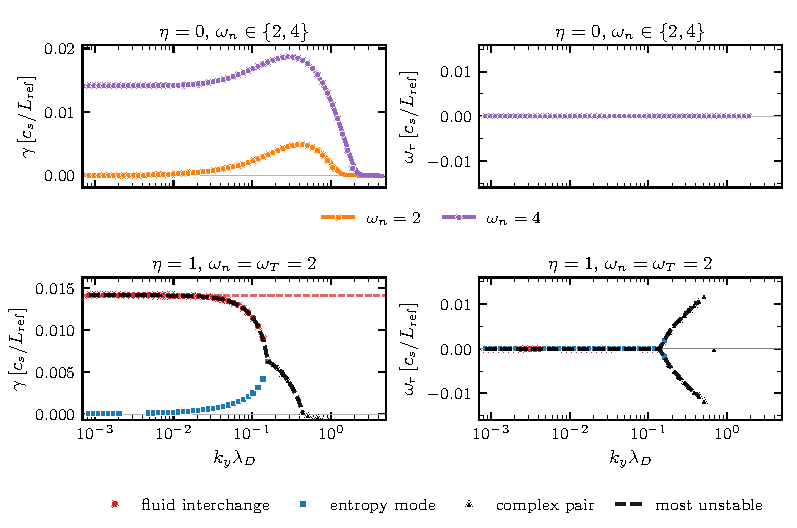
\includegraphics{plots/linear_combined_2x2.pdf}
\caption{Linear modes of the EP $Z$-pinch interchange vs.\ $k_y\lambda_D$. \textit{Left column:} growth rate $\gamma(k_y)$; \textit{right column:} real frequency $\omega_r(k_y)$. Markers: \gene\ eigenvalue scans; solid lines: the $Z$-pinch limit of the kinetic dispersion of \citet{MPH2018}. \textit{Top row:} $\eta = 0$ at $\omega_n = 2$ (orange) and $\omega_n = 4$ (purple); this mode is non-propagating, so $\omega_r = 0$. \textit{Bottom row:} $\eta = 1$ ($\omega_n = \omega_T = 2$); red circles: the fluid interchange (dominant branch); blue squares: the entropy mode (sub-dominant); black triangles: the complex-conjugate pair after the branch collision, shown as $\pm|\mathrm{Re}\,\omega|$; red dashed: the fluid-interchange rate \cref{eq:gamma_scaleinv}; black dashed: the most-unstable branch, the $Z$-pinch reference of \Cref{fig:dipole_csurf_kyscan}.}
\label{fig:linear_modes}
\end{figure}

We note that for all gradients considered here, the modes are stabilised by Debye screening at sufficiently small scale. The scale dependence of \Cref{fig:linear_modes} can be understood from the kinetic theory of \citet{MPH2018}, whose closed-form $Z$-pinch solution generalises the toroidal ion-temperature-gradient velocity integrals of \citet{Biglari1989} to the sign-opposite drifts of the pair plasma. For purely growing modes, the $Z$-pinch limit of the kinetic dispersion relation, \cref{eq:disp_BH} at $c_\mathrm{surf}\to1$, reads
\begin{equation}\label{eq:disp_zpinch}
\underbrace{\vphantom{\Bigl\langle}\;1 + (\kperp\lambdaD)^2\;}_{\text{shielding}}
\;=\;
\underbrace{\Bigl\langle\, J_0^2(\kperp\rho)\;
\frac{\Gamma^2 + u\,\Omega_*^T}{\Gamma^2 + u^2} \,\Bigr\rangle_{\!\bv}}_{\text{response}} ,
\end{equation}
where $\langle\cdot\rangle_\bv$ is the Maxwellian velocity average \cref{eq:app_fluid_vavg}, $u(\bv)$ the magnetic drift \cref{eq:vd} in units of its thermal value $\hat\omega_d$ (so that $\langle u\rangle_\bv = 1$), and $\Gamma \equiv \gamma/\hat\omega_d$, $\Omega_*^T \equiv \omega_*^T/\hat\omega_d$ the growth rate and the diamagnetic drive measured against that same drift frequency. Importantly, the diamagnetic frequency and the magnetic drift are both proportional to $k_y$, so those ratios are scale-independent. The right-hand side of \cref{eq:disp_zpinch} depends on the dimensionless drives and on velocity alone. The gyroaverage would be the exception, but $J_0\to1$ over the whole scan since $\kperp\rho \ll 1$ as a result of \cref{eq:ordering}. The right-hand side of \cref{eq:disp_zpinch} therefore has no scale, and every scale in the problem enters through the shielding term only.

The relation \cref{eq:disp_zpinch} carries the growth rate only through $\Gamma^2$. Thus, every unstable root is accompanied by a damped root of the same magnitude at the same wavenumber. The pairing also survives at complex frequency. In our simulations the two species have equal temperature and opposite charge, so the magnetic drift and the diamagnetic frequency, both proportional to $T/e_a$, change sign between them; the two resonant denominators of the linearised \cref{eq:dke} then combine into $\omega^2 - \omega_d^2$ and the dispersion function depends on the frequency only through $\omega^2$. Its roots therefore come in the set $\{\omega, -\omega, \omega^*, -\omega^*\}$, of which the two branches of \Cref{fig:linear_modes} show the growing half past their collision, at equal growth rate and opposite real frequency. The damped partner of a purely growing mode is an eigenmode of the collisionless system rather than an analytic continuation, because $\omega = \mathrm{i}\gamma$ never meets the drift resonance. What the pairing means for the saturated state is taken up in \cref{sec:rev_irr}.

The short-wavelength stabilisation is then simply the kinetic boundary \cref{eq:mph_kinetic} of \citet{MPH2018}. The kinetic boundary carries wavenumber only in its shielding term, so at fixed gradients it is crossed by raising $\kperp\lambdaD$ alone. The band ends where the shielding exceeds the response the drive can sustain. This is the pair plasma's counterpart of the finite-Larmor-radius cutoff of the electron--ion problem, but it acts on the opposite side of \cref{eq:disp_zpinch}. There the Bessel factor extinguishes the response, whereas here the screening term outgrows it. Since $\lambdaD\gg\rho$, screening matters long before the gyroaverage does and the finite-Larmor-radius cutoff is never reached at all.

The long-wavelength limit follows from a similar observation. At long wavelength the screening term is negligible and the shielding reduces to unity, so \cref{eq:disp_zpinch} fixes $\Gamma$. The mode grows at a fixed fraction of the drift frequency, and since that frequency is proportional to $k_y$, so is the growth rate. The exception is a mode fast enough to outrun the drift resonance, $\Gamma\gg u$. This branch is the fluid limit of \citet{MPH2018} (their equation~4.6).\footnote{It is possible to derive a closed set of fluid equations in this strongly-driven limit: at constant $|\bB|$ the bracket couples no velocity moments and the moment hierarchy closes. The resulting equations are isomorphic to the two-dimensional electrostatic limit of the fluid equations studied by \citet{ClarkeUnpub}, with the Debye polarisation in the role of the fluid inertia and the pressure-like moment in the role of the buoyancy. The derivation and the explicit mapping are given in \cref{app:fluid}.} Expanded in $u/\Gamma$, the unit terms on the two sides of \cref{eq:disp_zpinch} cancel, and the small screening term is balanced by the response correction, so that
\begin{equation}\label{eq:gamma_scaleinv_pre}
\Gamma^2 \;=\; \frac{\Omega_*(1+\eta) - 7/4}{(\kperp\lambdaD)^2}.
\end{equation}
The normalised growth rate then scales as $\kperp^{-1},$ hence,
\begin{equation} \label{eq:gamma_scaleinv}
    \gamma \propto \frac{k_{y}}{|\kperp|}.\end{equation}
The numerator of \cref{eq:gamma_scaleinv_pre} vanishes where \cref{eq:mph_fluid} places the fluid threshold, which this expansion therefore recovers, although $\Gamma\gg u$ requires $\Omega_*(1+\eta) - 7/4 \gg (\kperp\lambdaD)^2$, so the branch is described well above that threshold rather than at it. The rate depends on the drives only through the combination $\Omega_*(1+\eta)$, which is why $(\omega_n,\eta) = (4,0)$ and $(2,1)$ share a plateau in \Cref{fig:linear_modes}.

Unlike the typical electron--ion instability (and also the entropy mode), whose growth rate increases with $\kperp$, the rate \cref{eq:gamma_scaleinv} is unchanged under $\vk \to c\,\vk$. No inertial range therefore exists in the usual sense. Every mode on the plateau grows at the same rate, so the interchange supports no Kraichnan constant-flux cascade \citep{Kraichnan1967} (as with the idealised forward cascade of enstrophy in two-dimensional fluid turbulence, whose nonlinear turnover is likewise scale-independent). What saturates this branch therefore cannot be inferred from a scale-local cascade argument (see discussion in \cref{sec:saturation}). The ultraviolet end is supplied by the kinetic boundary \cref{eq:mph_kinetic}, at which Debye screening extinguishes the drive.

\subsection{Linear stability in the dipole}\label{sec:dipole_zpinch}

Linear instabilities in the dipole geometry are closely related to those in the $Z$-pinch. \Cref{fig:dipole_csurf_kyscan} shows the growth rate (left-hand side) and the mode frequency (right-hand side) as functions of $k_y \lambda_D$ at six values of $c_\mathrm{surf}$ for $\eta = 0$ (top row) and four for $\eta = 1$ (bottom row). The $Z$-pinch limit is $c_\mathrm{surf} \rightarrow 1$ and increasing $c_\mathrm{surf}$ increases the field-line variation of $|\bB|$ (see \cref{app:dipole_flux_tube}). The $Z$-pinch cases of \Cref{fig:linear_modes} are overplotted for reference. As $c_\mathrm{surf}$ increases, the stronger field-line variation of $|\bB|$ mildly enhances the $\eta = 0$ instability. The peak growth rate rises monotonically across the scan and the unstable band widens. At $\eta = 1$ the branch structure persists, with both the kinetic and the fluid interchange branches unstable. The dominant and sub-dominant eigenmode parallel structures are shown in \cref{app:dipole_lin_landscape}, and the comparison with the analytic dispersion is given in \cref{app:theory_compare}.

\begin{figure}
\centering
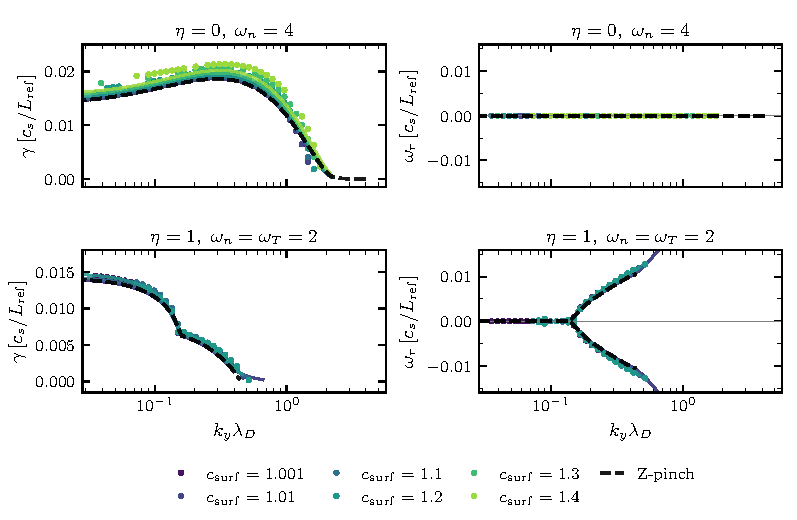
\includegraphics{plots/dipole_csurf_kyscan.pdf}
\caption{Linear modes of the dipole flux tube vs.\ $k_y\lambda_D$ at up to six values of $c_\mathrm{surf}$ (four at $\eta = 1$). \textit{Left column:} growth rate $\gamma(k_y)$; \textit{right column:} signed $\omega_r(k_y)$. Markers: \gene\ eigenvalue scans (dominant eigenmode); solid curves: dominant root of the bounce-harmonic dispersion of \cref{app:theory_compare}; black dashed: the $Z$-pinch reference ($c_\mathrm{surf} \to 1$). \textit{Top row:} $\eta = 0$ ($\omega_n = 4$). \textit{Bottom row:} $\eta = 1$ ($\omega_n = \omega_T = 2$); the dominant branch is the fluid interchange, shown as $\pm|\mathrm{Re}\,\omega|$ past its collision with the entropy mode.}
\label{fig:dipole_csurf_kyscan}
\end{figure}

The bounce-averaged dispersion relation is derived by taking the potential to be constant along the field line, $\phi \approx \bar\phi$, which is the flute closure. It is accurate in the near-$Z$-pinch limit and degrades as $c_\mathrm{surf}$ increases and the eigenmodes localise towards the field maxima. The production value $c_\mathrm{surf} = 1.10$ of \cref{sec:dipole_nl} sits just below the onset of that localisation, so the saturated parallel structure begins to depart from flute. What degrades is the accuracy of the dispersion relation, not the cascade predictions of \cref{sec:lambda_coupling}, which do not assume a flute potential.


\section{Nonlinear simulations in $Z$-pinch geometry}\label{sec:nonlinear}

The $Z$-pinch is the simplest closed-field-line geometry. Its field lines are circular with uniform $|\bB|$, so no particle is trapped and the orbit average of \cref{eq:orbit_avg} is an average along the field line for every particle. The nonlinearity then carries no pitch-angle dependence, and the perpendicular leg of the dual cascade can be tested on its own. We now check the theory developed in \cref{sec:theory} against nonlinear gyrokinetic simulations in this geometry. We measure the spectral transfer of the two invariants of~\cref{sec:invariants} directly, using free-energy diagnostics implemented in \gene\ by \citet{BanonNavarro2016}. \cref{sec:zonal} establishes the zonal-locked end state at weak drive (below the fluid interchange threshold), and \cref{sec:direct_cascade_flux} measures the dual cascade there. \cref{sec:nl_strong} shows that neither is lost above the fluid threshold \cref{eq:mph_fluid}, and \cref{sec:saturation} accounts for the residual transport that survives the zonal lock.

\subsection{Turbulence driven by the kinetic interchange (entropy mode)}\label{sec:nl_weak}

We begin by studying a case where the entropy mode is the only unstable mode in the system. We consider turbulence driven by a density gradient only ($\eta=0$) at a strength below the fluid threshold \cref{eq:mph_fluid}. The only drive is $\omega_n = 2$ [Point \circled{A} in \Cref{fig:stability_map}]. All simulations in this section are performed in the $Z$-pinch box of \Cref{tab:setup}. The Fj\o rtoft argument of \cref{sec:fjortoft} rests on the two invariants alone and places no condition on the drive. The dual cascade is expected here as much as at stronger drive.

\subsubsection{Approach to a zonal-flow dominated state}\label{sec:zonal}

The left-hand side of \Cref{fig:nonlinear_monitor} shows the time evolution of the free energy $W$ and of the electrostatic energy $E$, with $E$ split into its zonal and non-zonal parts. Both invariants grow exponentially through the linear phase and settle to a quasi-steady state. The right-hand side shows the zonal fraction
\begin{equation}\label{eq:zonal_fraction}
\mathcal{Z}_\varphi \;\equiv\; \frac{\sum_{k_x} |\hat\varphi_{k_x,\,0}|^2}{\sum_{\vk} |\hat\varphi_{\vk}|^2},
\end{equation}
which measures the share of the potential's power held in the zonal mode, with $\varphi \equiv e\phi/T$ the normalised potential of \cref{eq:poisson}. The zonal fraction rises steeply through saturation and then approaches unity slowly, reaching $\mathcal{Z}_\varphi \approx 0.97$ by the end of the simulation. This is consistent with collisionless zonal-flow stability and the absence of a tertiary instability (\cref{sec:zonal_stability}). The zonal mode carries no linear drive. At $k_y = 0$ the diamagnetic drive and the drift precession vanish with their explicit factor of $k_y$, leaving the $\vE \times \vB$ nonlinearity of \cref{eq:zonal_vorticity} as the only term able to change the zonal vorticity. The flow is driven by the Reynolds stress of the non-zonal turbulence, the zonal energy lifts off only as the primaries approach saturation and then grows considerably faster, as the secondary instability of \Cref{fig:phi_chi_snap} acting on a finite-amplitude primary. The saturated mean zonal profile $\bar v_y(x) = \partial_x \langle\varphi\rangle_y$ has several shear bands, with \textcolor{red}{a} root mean square shearing rate more than twice the linear growth rate. The structure of the zonal flow and the saturated state is discussed in \cref{app:epsy}. The non-zonal $|\varphi|^2$ sits an order of magnitude below the $k_y = 0$ component. On the left-hand side of \Cref{fig:nonlinear_monitor}, the zonal part of $E$ overtakes the non-zonal part as the flow locks, passes a maximum near the middle of the simulation and then relaxes slowly. The formation of strong zonal flows is accompanied by a reduction in the transport levels (see \Cref{fig:flux_timeseries} in \cref{sec:nl_strong}).

\begin{figure}
\centering
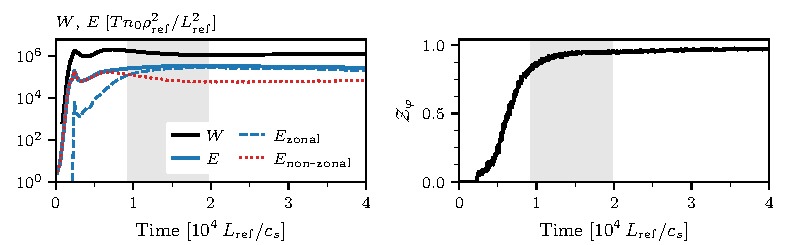
\includegraphics[width=\textwidth]{plots/nonlinear_invariants.pdf}
\caption{Time evolution for the weakly driven $Z$-pinch baseline ($\eta = 0$, $\omega_n = 2$). \textit{Left:} free energy $W$ (black) and electrostatic energy $E$ (blue solid), with $E$ split into zonal ($k_y = 0$, blue dashed) and non-zonal ($k_y > 0$, red dotted) parts. \textit{Right:} the zonal fraction $\mathcal{Z}_\varphi$ of \cref{eq:zonal_fraction}. The shaded band in both panels marks the cascade-averaging window of \Cref{fig:direct_cascade_flux}.}
\label{fig:nonlinear_monitor}
\end{figure}

\subsubsection{Direct measurement of the dual cascade}\label{sec:direct_cascade_flux}

The dual cascade can be observed directly from the simulation. The shell-decomposition diagnostic in \gene\ outputs the rate of change of each invariant's spectral density due to the $\vec{E} \times \vec{B}$ nonlinearity \citep{BanonNavarro2011, BanonNavarro2016},
\begin{equation}\label{eq:T_def}
T_X^\mathrm{NL}(\vec{k}; t) \;\equiv\; \left.\frac{\partial \hat X(\vec{k})}{\partial t}\right|_{\mathrm{NL}}, \qquad X \in \{E, Z\},
\end{equation}
with
\begin{equation}\label{eq:GK_W_E_defs}
\hat E(\vec k) = \frac{\lambdaD^2}{\rho_\mathrm{ref}^2}\, \kperp^2\, |\hat\phi_{\vec k}|^2 ,
\quad
\hat Z(\vec k) = \sum_a \int \rmd v_\parallel\, \rmd\mu\, \rmd z\; \frac{T_a\, |\hat g_a(\vec k)|^2}{2\, f_{a0}} .
\end{equation}
Here $\hat E$ is the Debye-screened electrostatic-energy density and $\hat Z$ is the species-summed entropy part of the free energy carried by the gyrocentre distribution $g_a$ of \cref{eq:gc_dist} [see also \cite{Schekochihin2008}]. The hatted densities follow the \gene\ normalisation, a uniform factor of two above the quadratic forms of \cref{sec:invariants}. The shares, directions, and shapes discussed below are unaffected. In the $Z$-pinch, $\hat Z$ is exactly the enstrophy-like invariant of \cref{sec:fjortoft}. Summing over the modes in each $\kperp$ shell gives the shell transfers $T_E^\mathrm{NL}(\kperp)$ and $T_Z^\mathrm{NL}(\kperp)$, from which we construct the cumulative spectral fluxes
\begin{equation}\label{eq:Pi_def}
T_X^\mathrm{NL}(\kperp) \;=\; \sum_{\vec k \,\in\, \mathrm{shell}(\kperp)} T_X^\mathrm{NL}(\vec k),
\qquad
\Pi_X(\kperp) \;\equiv\; -\!\!\sum_{k' \,\le\, \kperp} T_X^\mathrm{NL}(k') ,
\qquad X \in \{E, Z\}.
\end{equation}
The flux $\Pi_X(\kperp)$ is the net rate at which the nonlinearity moves $X$ out of the modes below $\kperp$. A positive $\Pi_X$ is forward transfer towards smaller scales and a negative one inverse transfer towards larger scales.

\Cref{fig:direct_cascade_flux} shows $\Pi_E$ (left-hand side) and $\Pi_Z$ (right-hand side), time-averaged over the window shaded in \Cref{fig:nonlinear_monitor}. The two invariants are transferred in opposite directions as anticipated in \cref{sec:fjortoft}. The electrostatic energy cascades inversely. The transfer $T_E^\mathrm{NL}$ is positive at the largest scales and negative across the rest of the band, so the cumulative flux $\Pi_E$ is negative throughout the transfer band. It peaks in magnitude near the injection scale at $\kperp\lambdaD \approx 0.33$ and falls through zero near $\kperp\lambdaD \approx 1.3$. The entropy cascades forward. The cumulative flux $\Pi_Z$ is positive and relatively flat over $\kperp\lambdaD \in [0.64, 1.27]$. There is a constant-flux range across which the nonlinearity delivers entropy to the dissipation range at a scale-independent rate. Both fluxes return to zero at the edge of the resolved range, as conservation of each invariant by the nonlinearity requires.

The dual cascade is active throughout the simulation. However, the two cascades differ in how they terminate. The forward flux of $Z$ ends in a sink. Free energy is absorbed by $\varepsilon_v$ at small scales, and so the $Z$ spectrum is statistically steady while the flux passes through it. The inverse flux of $E$ ends in a reservoir. Nothing destroys what it delivers and the condensate grows at the delivery rate. \gene\ evolves each invariant according to
\begin{equation}\label{eq:per_mode_budget}
\partial_t X(\kperp) \;=\; T_X^\mathrm{drive}(\kperp) + T_X^\mathrm{lin}(\kperp) + T_X^\mathrm{diss}(\kperp) + T_X^\mathrm{NL}(\kperp),
\end{equation}
where the linear group collects the curvature drift and parallel streaming, and the dissipative group collects collisions and hyperdiffusion. In the $Z$-pinch runs, the parallel and collisional terms are absent (\Cref{tab:setup}), so the removal is by the $\vpar$ hyperdiffusion $\varepsilon_v$ alone. The gradients inject $Z$ and the nonlinearity carries it forward until $\varepsilon_v$ removes it at high $\kperp$. As such, the terms of \cref{eq:per_mode_budget} can balance and the flat range of $\Pi_Z$ is the signature of that balance. The $\kperp$ selectivity of this removal is inherited rather than intrinsic since the sink acts on $\vpar$ alone. The magnetic-drift frequency depends on velocity through \cref{eq:vd}. Hence, fine $\vpar$ structure is generated by phase mixing through the drift resonance at a rate proportional to $k_y$ and only modes of high $k_y$ reach $\vpar$ scales fine enough for $\varepsilon_v$ to act on within a turnover. Beyond the kinetic boundary \cref{eq:mph_kinetic}, at $\kperp\lambdaD \approx 1.5$ for this drive, the shielding exceeds the response the drive can sustain and the modes are net drift-Landau-damped \citep{MPH2018} and their free energy passes into fine $\vpar$ structure that $\varepsilon_v$ erases. The plateau of $\Pi_Z$ ends just below this boundary and so the removal sits where the linear theory places it. The electrostatic energy admits no such balance. It has no direct source since the diamagnetic drive cancelling from its budget in the species sum (\cref{sec:invariants}). Instead, $E$ is fed only by the curvature-mediated conversion from $Z = W - E$, for which $T_E^\mathrm{curv} = -T_Z^\mathrm{curv}$, the drift term being a perfect $\alpha$-derivative that drops out of $\rmd W/\rmd t$ altogether. $E$ also has no sink since the hyperdiffusion carries no charge moment \cref{eq:hypv_charge} and the zonal flow is undamped \cref{eq:zonal_vorticity}. What the conversion supplies and the inverse transfer delivers can only accumulate at the largest scales. The measured $\Pi_E$ is that accumulation in progress. Accordingly, $\Pi_E$ has no constant-flux range of its own and the zonal part of $E$ is still rising across the averaging window (\Cref{fig:nonlinear_monitor}). The inverse leg measured here belongs to the formation of the condensate rather than to a stationary state.

\begin{figure}
\centering
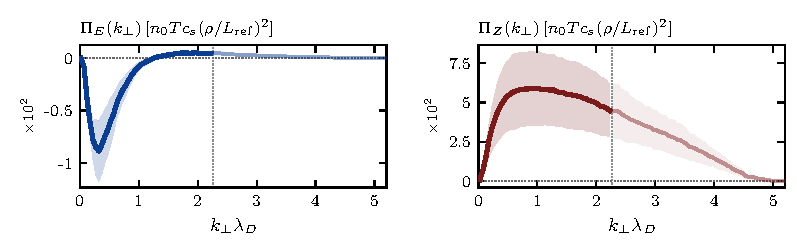
\includegraphics[width=\textwidth]{plots/spectral_flux_direct.pdf}
\caption{Cumulative spectral fluxes of \cref{eq:Pi_def} for the baseline $Z$-pinch run ($\eta = 0$, $\omega_n = 2$), averaged over $t \approx 8950$--$20000\, L_\mathrm{ref}/c_s$, the window marked in \Cref{fig:nonlinear_monitor}. \textit{Left:} $\Pi_E(\kperp)$. \textit{Right:} $\Pi_Z(\kperp)$. Shaded bands: scatter in one standard deviation. Curves are drawn solid to the largest complete $\kperp$ shell (dotted vertical) and faded beyond it, where the rectangular box no longer contains every mode of a shell and the curve is only a partial-shell estimate.}
\label{fig:direct_cascade_flux}
\end{figure}

\subsection{Turbulence driven by the scale-independent interchange}\label{sec:nl_strong}\label{sec:nl_eta1}

We now study a case where the fluid interchange mode is unstable. We consider turbulence driven by gradients of both temperature and density ($\eta = 1$) with $\omega_n = \omega_T = 2$ [Point \circled{B} in \Cref{fig:stability_map}]. This simulation sits above the fluid threshold \cref{eq:mph_fluid} and so occupies the regime in which the interchange grows at the scale-independent rate \cref{eq:gamma_scaleinv}. These simulations use the same $Z$-pinch box of \Cref{tab:setup}. The $\eta = 1$ run contains the same dual cascade as the $\eta=0$ run (not shown). Once again $\Pi_E$ and $\Pi_Z$ can be directly measured as having opposite sign as in \Cref{fig:direct_cascade_flux}. The directions are set by the invariants and by the bracket that conserves them and not by the strength of the drive \cref{sec:fjortoft}.

It is interesting to compare the transport in the two cases. \Cref{fig:flux_timeseries} shows the species-summed, heat flux (top row), particle flux (middle row), and nonlinear invariants (bottom row) for the $\eta = 0$ run (left-hand column) and the $\eta = 1$ run (right-hand column). Both runs saturate to a zonal-flow-dominated state, through exponential growth and a zonal-suppressed tail. In both regimes the primaries grow past the level the system can hold, building up a store of free energy from the gradients. The secondary instability then builds the zonal condensate on that finite-amplitude primary, and the condensate quenches the turbulence. The store is dissipated afterwards at a rate set by how fast the drift resonance can phase-mix structure down to velocity-space scales where the sink can remove it [\cref{app:epsy}].

The free energy overshoot is slight at $\eta = 0$ and very large at $\eta = 1$ [\Cref{fig:flux_timeseries}]; the free energy passes its saturated level by an order unity amount in the weakly driven run and by six orders of magnitude in the strongly driven one. At $\eta = 0$ (weakly driven) the drive sits below the fluid threshold \cref{eq:mph_fluid}, so the growing mode is the resonant kinetic one: it occupies a band around a definite binormal scale, and the drift resonance damps it while it grows, so free energy is delivered to the sink as fast as the gradients supply it and little accumulates. At $\eta = 1$ (strongly driven) the drive sits above that threshold, the growth rate is the same at every scale \cref{eq:gamma_scaleinv}, so the whole spectrum grows at once and the fluid branch is fast enough to outrun the drift resonance, the only route by which free energy reaches the velocity-space scales where the sink removes it \cref{sec:gk_to_dke}. Thus in the strong-driven case, free energy accumulates without being dissipated, and afterwards has to drain slowly by the route it outran to reach a steady state. That is why only the strongly driven run is still relaxing (to a finite floor) at the end of the simulation (see \cref{fig:flux_timeseries} and discussion in \cref{sec:saturation,sec:rev_irr}).

The strongly-driven case also carries a persistent large-scale oscillation in the instantaneous fluxes about the slowly falling level that tracks the free energy dissipation. This oscillation is not the predator--prey cycling of zonally regulated fluid turbulence, in which each quiescent period is timed by the slow decay of the zonal flow and each burst restores it \citep{ClarkeUnpub}. The zonal flow here is undamped \cref{eq:zonal_vorticity} and stays locked through the oscillation. Instead, the oscillations in the fluxes are due to the rapid exchange of electrostatic energy. Over each cycle the zonal and non-zonal parts (large-scale vortices in \Cref{fig:phi_chi_snap}) of the electrostatic energy exchange in anti-phase at nearly constant total. The velocity-space sink in the simulations cannot remove the electrostatic energy directly \cref{eq:hypv_charge} and so this exchange is conservative to better than a hundredth per cycle. A vortex carries fluid outward through one half of its circulation and back inward through the other, so the instantaneous flux alternates in sign as the pattern turns, and does so throughout the simulation [\Cref{fig:flux_timeseries}]. This rapid oscillation sits on top of the slow decay of the fluxes that tracks the free energy which the sink does remove. The free energy \textcolor{red}{[\Cref{fig:flux_timeseries}, bottom right]} and its sink \textcolor{red}{[\Cref{fig:energy_balance_vs_drive}, right-hand column]} carry no per-cycle signature: the store drains monotonically through many cycles, a single long relaxation rather than a predator--prey loop. The cycle frequency rises with the zonal amplitude, consistent with advection of the coherent vortices by the zonal flow. The cycling is therefore an oscillation of the surviving fluctuations on the locked condensate, not a sequence of suppression and regrowth events. \textcolor{red}{We call these rapid oscillations of the fluxes vortex breathing. Each cycle the vortices gain and lose electrostatic energy as they exchange it with the condensate and the flux alternates in sign. The period of the vortex breathing is one to two e-folding times of the linear interchange, the $\vE \times \vB$ turnover time of the large-scale vortices, whereas the store drains on a timescale two orders of magnitude longer and lengthening; the breathing is the free dynamics of the coherent vortices, sitting on top of the slow drain of the store.}

Interestingly, at the stronger drive, the two transport channels do not arrest with the same sign as they did in the $\eta=0$ case. At $\eta = 1$ the particle flux\textcolor{red}{, averaged over the vortex breathing,} reverses to a small inward (up-gradient) pinch, while the heat channel carries the outward residual. In a statistically steady state it is not each flux that is fixed but the injection term of \cref{eq:W_balance}; a gradient-weighted combination of the two that is pinned by the free-energy dissipation rate \citep{KrommesHu1994, Sugama1996}. At $\eta = 0$ the density gradient alone injects free energy and so the combination reduces to $\Gamma_{\rm es}$ itself and the particle flux arrests at a positive floor of its own.

An inward particle pinch in a confined pair plasma has been anticipated previously on several grounds. Quasilinear theory predicts an up-gradient particle flux near marginal stability whenever $\eta > 2/3$ \citep{HelanderConnor2016}. \citet{MPH2018} conjectured that the interchange modes studied here could supply the background turbulence such a pinch requires and this seems to be the case in the simulations reported here. The effect also has precedent in electron--ion plasmas. Turbulent-equipartition arguments predict inward convection from the conservation of adiabatic invariants \citep{Yankov1994, Isichenko1995, Isichenko1996}. In closed-field-line systems in particular, gyrokinetic simulations of dipole-like geometry find a particle pinch \citep{Kobayashi2010} and such pinches have even been measured experimentally. LDX has measured a turbulent inward pinch \citep{BoxerLDX2010} and RT-1 a peaked density profile \citep{Saitoh2011}.

The real space structure of the turbulence is also different between the two cases. \Cref{fig:phi_chi_snap} follows the formation of the saturated state in real space. In both columns the modes grow as radially extended streamers which steepen and buckle as the secondary instability sets in. The zonally-dominated state emerges that emerges from the secondary is the zonal condensate whose rise the overlays of \Cref{fig:flux_timeseries} track. The stronger drive reaches each stage sooner. Interestingly, the two columns of \Cref{fig:phi_chi_snap} differ in how the streamers break. At $\eta = 0$ (left-hand column) they carry the fine binormal scale of the entropy mode and break into a band of small vortices which the zonal flow then absorbs. At $\eta = 1$ (right-hand column) they instead roll up into large-scale coherent vortices [gold dashed contours] that persist into the developed state as cores embedded in the condensate. The entropy mode peaks at a definite binormal scale (\Cref{fig:linear_modes}) whereas on the scale-independent plateau every scale grows at the same rate \cref{eq:gamma_scaleinv} and no binormal scale is singled out.

\begin{figure}
\centering
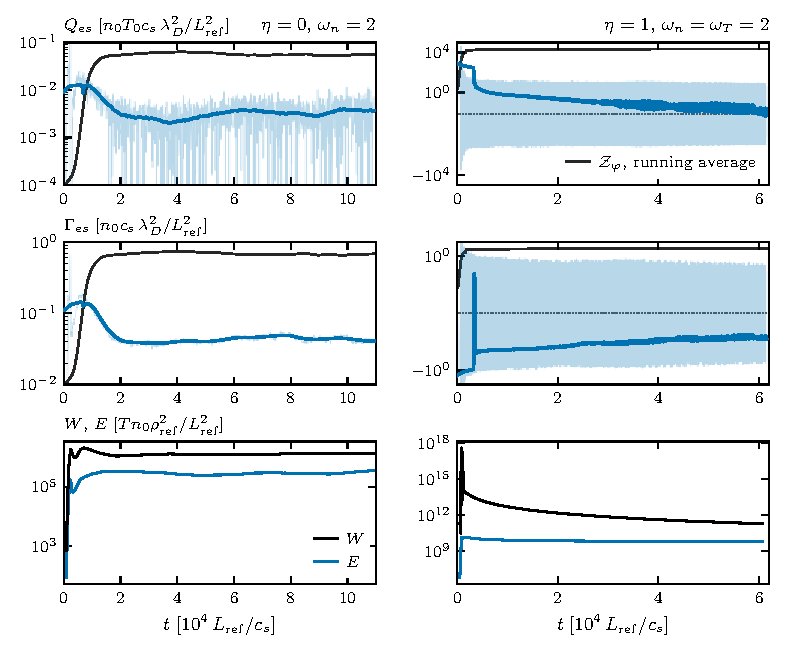
\includegraphics[width=\textwidth]{plots/eta_scan_saturation.pdf}
\caption{Species-summed electrostatic fluxes of \cref{eq:flux_def} for the two $Z$-pinch runs, in mixing-length units built on $\lambdaD$. Velocity-space dissipation only ($\varepsilon_y = 0$, \Cref{tab:setup}). \textit{Top row:} heat flux $Q_{es}(t)$. \textit{Middle row:} particle flux $\Gamma_{es}(t)$. \textit{Bottom row:} the free energy $W$ (black) and the electrostatic energy $E$ (blue), as the left-hand panel of \Cref{fig:nonlinear_monitor}. \textit{Left column:} $\eta = 0$, $\omega_n = 2$. \textit{Right column:} $\eta = 1$, $\omega_n = \omega_T = 2$. Bold, the running time-average; faded behind it, the instantaneous flux. The right column is drawn on a symmetric log scale with a dotted line at zero, the left on a log scale. The black trace ($0$--$1$ scale) on the flux panels is the running-average zonal fraction $\mathcal{Z}_\varphi$ of \cref{eq:zonal_fraction}.}
\label{fig:flux_timeseries}
\end{figure}

\begin{figure}
\centering
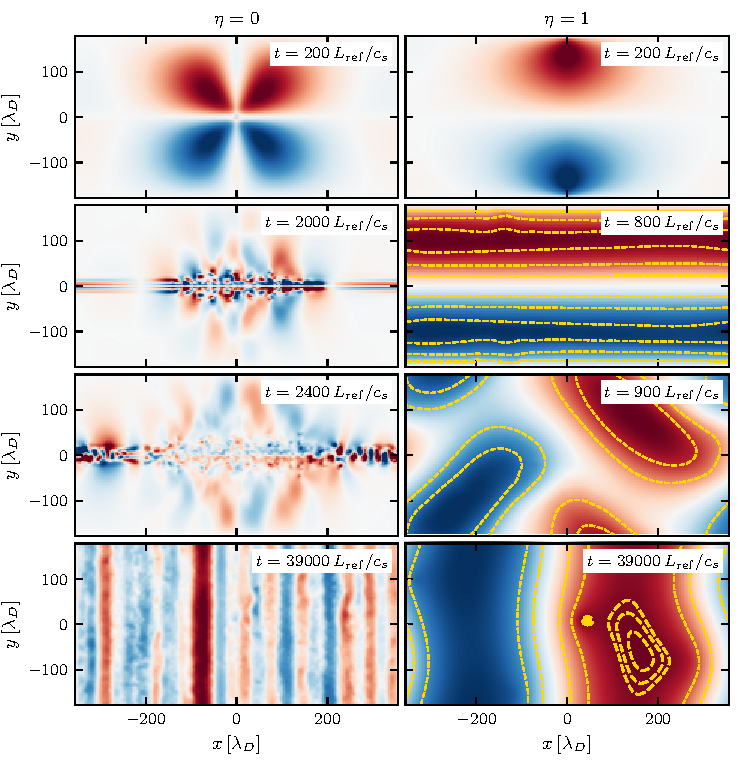
\includegraphics{plots/zpinch_morph_evolution.pdf}
\caption{Formation of the $Z$-pinch saturated state: normalised potential $\varphi(x, y)$ of \cref{eq:zonal_fraction} in a radially elongated box ($2\!:\!1$ in $x\!:\!y$). \textit{Left column:} $\eta = 0$, $\omega_n = 2$. \textit{Right column:} $\eta = 1$, $\omega_n = \omega_T = 2$. Rows, top to bottom: close to the initial condition, formation of streamers, the secondary instability, the developed state. The two runs share their initial perturbation. The top and bottom rows are at common times, the middle two matched by stage. Colour scales saturate at the 99th percentile of each panel. Gold dashed contours in the $\eta = 1$ column mark fixed fractions of each panel's colour scale, with closed rings added around the strongest vortex cores in the developed row.}
\label{fig:phi_chi_snap}
\end{figure}



\subsection{The transport floor}\label{sec:saturation}

The transport fluxes (\Cref{fig:flux_timeseries}) approach a finite floor. In our simulations this floor exists because the zonal flows are able to suppress the fluctuation band without stabilising it completely. This is explored in \cref{app:epsy}. The main result is that, when reseeded at $10^{-8}$ of its former amplitude, the non-zonal band still regrows exponentially with an effective growth rate of $\gamma_\mathrm{eff} \approx 0.66\,\gamma_\mathrm{lin}$ where $\gamma_\mathrm{lin}$ is the peak linear growth rate at a given drive. The regrowth localises in the zero-shear lanes that each zonal profile contains (\cref{app:epsy_regrowth}). The Dimits shift shows the same coexistence of strong zonal regulation with incomplete stabilisation \citep{Dimits2000, StOnge2017, Ivanov2020}. A band sheared but not extinguished keeps drawing on the gradients. The bracket $\pbra{\bar\phi}{h_a}$ moves both invariants between shells but removes neither,
\begin{equation}\label{eq:nl_conserve}
\sum_{\vec k} T_X^\mathrm{NL}(\vec k) \;=\; 0, \qquad X \in \{Z, E\},
\end{equation}
the sum running over all modes, and so in a steady state the dissipative sink must remove free energy as fast as the drive injects it \citep{KrommesHu1994, WatanabeSugama2004, CandyWaltz2006}. This finite dissipation pins a finite gradient-weighted combination of the fluxes through the free-energy balance \cref{eq:W_balance}.

Although our simulations do not reach it, a zonally dominated transport-free state does exist and such a state is a fixed point of the dynamics: with the non-zonal sector zeroed at a single timestep and then allowed to evolve freely, the flux stays identically zero and the zonal flows persist (\cref{app:epsy_attractor}).

The finite transport floor does not seem a threat to confinement: at the weaker drive the heat channel carries a small outward residual a few parts in a thousand of the mixing-length level built on $\lambdaD$ (\Cref{fig:flux_timeseries}).  At $\eta = 1$ the particle channel runs inward (\cref{sec:nl_eta1}) an up-gradient pinch that peaks the density profile and could be beneficial for plasma fuelling. Zero transport remains available below the instability thresholds and in the nonlinearly stable region identified by \cite{Helander2017}, but reaching that region requires the density and temperature gradients to relax together, a relaxation these fixed-gradient simulations do not allow. 

\subsection{Reversible and irreversible dynamics at the floor}\label{sec:rev_irr}

The floor of \cref{sec:saturation} \textcolor{red}{(and the stationarity, or lack thereof, of the simulations)} can be characterised by the energy balance of the saturated state as well as by the transport it carries.\footnote{\textcolor{red}{\Cref{app:epsy} takes up in detail what this section measures: the dissipation scans that fix the floor, the budget resolved by mode and by binormal wavenumber, the definitions \cref{eq:gross_net} of the gross and the net drive used below, and the free decay of the strongly driven store.}} For each invariant $X \in \{Z, E\}$ we split its rate of change into a reversible part \textcolor{red}{(due to the collisionless, time-reversible gyrokinetic dynamics)} and an irreversible part \textcolor{red}{(due to the dissipation)},
\begin{equation}\label{eq:rev_irr}
\mathcal{R}_X \;\equiv\; \sum_{\vec k}\bigl[\,T_X^\mathrm{drive}(\vec k) + T_X^\mathrm{lin}(\vec k)\,\bigr],
\qquad
\mathcal{I}_X \;\equiv\; \sum_{\vec k}\,T_X^\mathrm{diss}(\vec k),
\end{equation}
where $T_X^\mathrm{drive}$ is the contribution of the gradient-drive term of \cref{eq:dke} to the budget of $X$ \cref{eq:GK_W_E_defs}, $T_X^\mathrm{lin}$ that of the magnetic-drift term, the only linear channel the $Z$-pinch has, and $T_X^\mathrm{diss}$ that of the velocity-space sink, the only dissipation these runs carry (\Cref{tab:setup}). The drift term conserves the free energy $W = Z + E$ but neither invariant separately. Its contribution to the two budgets is equal and opposite and the mode-summed $T_Z^\mathrm{lin}$ and $T_E^\mathrm{lin}$ cancel identically, as the perfect $\alpha$-derivative of \cref{sec:invariants} requires. \textcolor{red}{The nonlinear bracket appears in neither rate, since it conserves both invariants \cref{eq:nl_conserve}; it moves them between modes, and it does so far faster than the sink acts. This is the large sloshing between modes that overshadows the residual net fluxes going to dissipation scales (\Cref{fig:flux_timeseries})} 

A quasi-steady state balances $\mathcal{R}_X$ against $\mathcal{I}_X$ on average. \textcolor{red}{Each invariant's budget has three terms: what the gradients put in (drive); what the drift moves between $Z$ and $E$ (lin); and what the sink takes out (diss). Of these channels, only the sink is irreversible. At $\eta = 0$ the nonlinearity transfers free energy between modes at a rate that is approximately two orders of magnitude larger than the rate of injection, while the net it leaves at any one $k_y$ is comparable to the injection there. The exchange with the gradients is reversible in a similar way, the paired growing and damped eigenmodes of \cref{sec:linear} drawing free energy and returning it. In both of these exchanges, far more free energy passes back and forth than is retained, and it is the retained part, averaged over time, that the dissipation has to match in steady state.} 

\Cref{fig:energy_balance_vs_drive} shows the two rates of \cref{eq:rev_irr} for each invariant, and \Cref{fig:sink_persistence} follows their ratio through each simulation. The two columns of \Cref{fig:energy_balance_vs_drive} show the same budget in two different states of the turbulence. In the weakly-driven system (left-hand column) the budget is that of a driven steady state: the drive and the sink balance in $Z$, while $\mathcal{R}_E$ exceeds $\mathcal{I}_E$ by an order of magnitude, since no channel dissipates $E$ directly. Above the fluid threshold (right-hand column) the window sits in the relaxation that follows the saturation burst, and dissipation dominates both budgets: the burst stored far more free energy than the drive injects over the window, the sink is still draining that store, and the $Z$ ratio of \Cref{fig:sink_persistence} climbs monotonically from nearly five decades below unity by about two orders of magnitude, approaching the balance the baseline already sits at from the dissipation-dominated side. In the bottom row of \Cref{fig:energy_balance_vs_drive} the two $E$ rates cross within the simulation, $\mathcal{R}_E$ ending above $\mathcal{I}_E$, while $\mathcal{R}_Z$ stays far below $\mathcal{I}_Z$ throughout. The transport fluxes fall as the store of free energy is slowly dissipated, so the strongly driven state is not transport-arrested on the timescale simulated. The relaxation timescale lengthens throughout the simulation as anticipated by the free-decay law: the drain slows as the store empties. The sink falls with the store, by two orders of magnitude, because there is less free energy to remove and because more of what remains sits in the zonal modes the sink does not reach. The drive meanwhile is steady. A steady state requires the drive and the sink to balance, and that balance fixes a finite store, and a finite flux with it, of the kind the $\eta = 0$ column of \Cref{fig:flux_timeseries} has already reached. \textcolor{red}{A steady state balances $W$ rather than $Z$ on its own. The drift term only moves free energy between $Z$ and $E$, so what must balance the total dissipation is the injection $\mathcal{R}_Z + \mathcal{R}_E$ of \cref{eq:W_balance}, and \Cref{fig:sink_persistence} draws that ratio beside the one for $Z$. At $\eta = 0$ the two ratios coincide at unity: with no temperature gradient the drift term has nothing to exchange, so $Z$ carries the whole budget. At $\eta = 1$ they separate by more than a decade, this is because $\langle|\mathcal{R}_Z|\rangle$ counts the reversible oscillation of the vortex breathing while the injection is the small residue that oscillation leaves.}

\begin{figure}
\centering
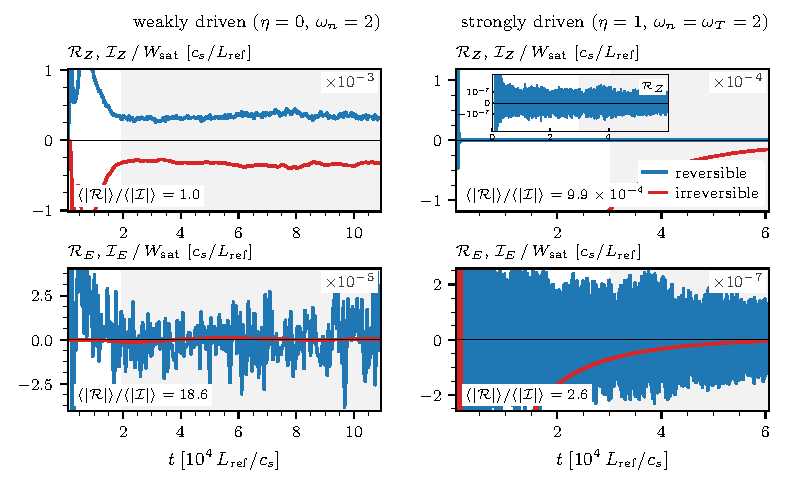
\includegraphics[width=\textwidth]{plots/zpinch_energy_balance_vs_drive.pdf}
\caption{The reversible and irreversible contributions to the budget of each invariant \cref{eq:rev_irr}, as raw rates normalised by the saturated free energy: blue, $\mathcal{R}_X$; red, $\mathcal{I}_X$. \textit{Top row:} $Z$. \textit{Bottom row:} $E$. \textit{Left-hand column:} the weakly driven baseline. \textit{Right-hand column:} above the fluid threshold, a post-burst relaxation rather than a saturated average. Shading marks each column's averaging window. The window ratio of mean magnitudes $\langle|\mathcal{R}|\rangle/\langle|\mathcal{I}|\rangle$ is annotated in each panel. The inset shows $\mathcal{R}_Z$ of the strongly driven run at its own scale, three orders of magnitude below that of the panel. After the saturation burst it oscillates about \textcolor{red}{a small positive} mean with no secular trend.}
\label{fig:energy_balance_vs_drive}
\end{figure}

\begin{figure}
\centering
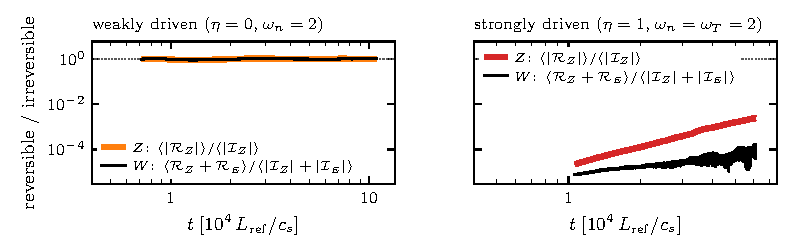
\includegraphics{plots/sink_persistence.pdf}
\caption{\textcolor{red}{The reversible rate over the irreversible one followed through each simulation. \textit{Left-hand side:} the weakly driven baseline. \textit{Right-hand side:} above the fluid threshold. Each panel carries the ratio for $Z$, the pair of rates of \cref{eq:rev_irr} annotated in \Cref{fig:energy_balance_vs_drive}, and the ratio for $W$, the injection of \cref{eq:W_balance} over the total dissipation of both invariants; both are labelled in the panel.} All means are sliding time-window means over $8\%$ of each simulation. Dotted, unity, where the reversible rate matches the irreversible one. Both axes logarithmic.}
\label{fig:sink_persistence}
\end{figure}

The same balance explains the flux oscillation of \cref{sec:nl_eta1}. The background gradients are the only source of free energy in these simulations, and they give it up only when the turbulence carries heat and particles down them, which is why the drive term of \cref{eq:rev_irr} is the gradient-weighted combination of the two fluxes \cref{eq:W_balance}: transport down the gradient adds free energy to the fluctuations, and transport up the gradient hands it back. At $\eta = 1$ the fluxes change sign as the vortices turn over, so the drive term changes sign with them, and the free energy the gradients have given to the fluctuations is handed back half a turn later [\Cref{fig:flux_timeseries}, bottom right]. What the sink removes is therefore the time-averaged drive and not the oscillation, and at $\eta = 1$ that average is a small residue of a much larger exchange, the residual flux being the same residue read in the transport channel.

\textcolor{red}{\Cref{fig:budget_rates} resolves the budget of \cref{eq:rev_irr} in $k_y.$ Written for $W$, whose budget the drift term drops out of, and summed over $k_x$, \cref{eq:per_mode_budget} is}
\begin{equation}\label{eq:per_mode_W}
\partial_t W(k_y) \;=\; T_W^\mathrm{drive}(k_y) \;+\; T_W^\mathrm{NL}(k_y) \;-\; \bigl|T_W^\mathrm{diss}(k_y)\bigr| ,
\end{equation}
\textcolor{red}{and dividing through by the free energy of the same $k_y$ turns every term into a rate,}
\begin{equation}\label{eq:per_mode_rates}
\underbrace{\frac{\rmd \ln W(k_y)}{\rmd t}}_{\text{what the mode holds}}
\;=\; \underbrace{\frac{T_W^\mathrm{drive}(k_y)}{W(k_y)}}_{\text{gradients}}
\;+\; \underbrace{\frac{T_W^\mathrm{NL}(k_y)}{W(k_y)}}_{\text{other modes}}
\;-\; \underbrace{\frac{\bigl|T_W^\mathrm{diss}(k_y)\bigr|}{W(k_y)}}_{\text{sink}}\,.
\end{equation}
{\color{red}The left-hand side is the rate at which the mode's own free energy grows or falls; on the right are the rates at which the gradients supply that free energy, the other modes supply it (via the nonlinearity), and the sink removes it. All four rates are drawn in \Cref{fig:budget_rates}, for the $\eta=0$ (left-hand side) and $\eta=1$ (right-hand side) cases, against the rate at which a fluctuation made of the unstable eigenmode, $\rmd \ln W/\rmd t = 2\gamma_\mathrm{lin}(k_y)$, since $W$ grows at twice the mode rate and the gradients are its only linear source. The transfer is not measured directly mode by mode at $\eta = 1$, its instantaneous value there being some hundred and seventy times its own window mean, so in both panels it is drawn as the term that closes \cref{eq:per_mode_rates}, dotted where it falls within the spread of three estimators of the store's decay. At $\eta = 0$, where the transfer can also be measured directly, the closure and the measurement agree to within a few per cent and the closure conserves free energy over the spectrum to two parts in a thousand. The two runs differ in which term in \cref{eq:per_mode_rates} balances the sink.


At $\eta = 0$ the free energy per mode is steady: on the left-hand side of \Cref{fig:budget_rates} the rate at which each mode's free energy changes lies orders of magnitude below every other term. The gradients and the transfer between modes balance the sink between them. At the longest wavelength the gradients supply some three times what the local sink removes, and the transfer carries the excess to short wavelength, where the drive falls through the sink's rate near $k_y\lambdaD \approx 0.9$ and the transfer makes up the difference instead. The turbulence retains about half of what it exchanges with the gradients, and between a third and two thirds mode by mode.} The transport floor is therefore a flow through wavenumber rather than a balance struck at any single scale. The zonal modes stand outside that flow: they hold most of both invariants, but they take no drive, and their net exchange of free energy with the rest of the spectrum is about a hundredth of the injection. The rapid anti-phase exchange of \cref{sec:nl_eta1} is in the electrostatic energy, and the free-energy budget carries no signature of that exchange.

{\color{red}At $\eta = 1$ the store of free energy in each mode is still being spent. Over the linearly unstable range of $k_y$ the right-hand side of \Cref{fig:budget_rates} shows the decay rate lying on the sink's rate, each mode losing free energy at the rate its own dissipation removes it, while the drive lies four to five orders of magnitude below both. Above the fluid threshold, what the sink removes is the free energy the saturation burst stored and not anything the gradients supply now. The drive is nonetheless positive at every $k_y$ the simulation resolves, so the gradients are still injecting, just far too slowly to hold the store up. Above the linear cutoff the decay rate falls away and the sink is balanced by the transfer instead, which supplies essentially all of it: those modes hold their free energy steady while their dissipation continues, so what the sink takes from them is replaced by transfer from the unstable modes below. The asymptotic state has a $Z$-dissipation floor and a transport floor, as at $\eta = 0$, and the simulation ends far short of it: the store it stops at is some five hundred times the store its own injection can sustain, and the free-decay law puts that state twenty simulation lengths away [\cref{app:epsy_decay}]

Most of what the gradients hand over comes straight back, and more so at the strong drive. The net drive counts the exchange with the gradients with its sign, so that free energy the gradients give and later take back cancels out of the net, while the gross drive counts every gain and every loss without regard to sign \cref{eq:gross_net}. The gap between the two rates is the free energy that passes back and forth within the averaging window and never reaches the sink, and that gap is what separates the two runs: at $\eta = 0$ the gross drive exceeds the net by about a factor of two, at $\eta = 1$ by some three hundred. Both rates are set against the linear growth rate in \cref{app:epsy_kspace}.}

\begin{figure}
\centering
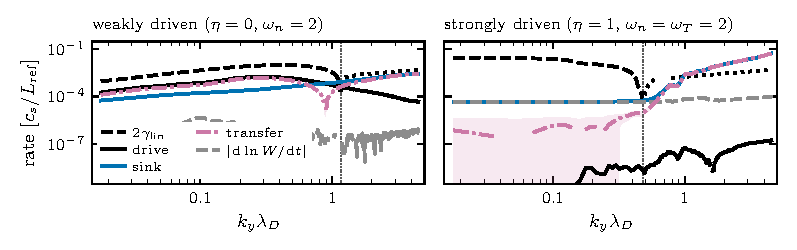
\includegraphics{plots/budget_rates.pdf}
\caption{\textcolor{red}{Every term of the per-$k_y$ free-energy budget \cref{eq:per_mode_rates} as a rate, each channel divided by the free energy of the same $k_y$ and time-averaged. \textit{Left-hand side:} the weakly driven baseline, over the arrested floor. \textit{Right-hand side:} above the fluid threshold, over the drainage. Each panel carries the drive, the sink, the transfer between modes and the rate at which the mode's own free energy changes, against the linear reference $2\gamma_\mathrm{lin}(k_y)$, dashed where the linear mode grows and dotted where it is damped. The transfer is the term that closes the budget; where it does not exceed the spread of three estimators of the store's decay it is drawn dotted, with that spread shaded. Curves carry magnitudes and break where a term changes sign; the transfer is negative at long wavelength and positive at short, and the store falls at $\eta = 1$ where at $\eta = 0$ it is steady. The vertical dotted line marks where the linear growth rate changes sign. Both axes logarithmic.}}
\label{fig:budget_rates}
\end{figure}

A steady state requires the irreversible channel. The arrested flux is insensitive to the strength of the velocity-space sink and to the velocity-space resolution [\cref{app:convergence}]. With no sink at all there is no steady state: the free energy grows steadily while the transport remains finite [\Cref{fig:sink_endstates}]. Neither drive admits a floor without dissipation: at $\eta = 0$ the injection of \cref{eq:W_balance} is the particle flux alone, one channel of one sign, and at $\eta = 1$ the inward particle channel removes under a tenth of what the temperature channel injects. A perpendicular sink is different in kind, acting on the transport-carrying fields directly, although a factor of twenty in the perpendicular coefficient leaves the arrested level within a factor of about two of the velocity-space floor [\Cref{fig:epsy_scan}]. The level therefore depends on which kind of dissipation acts, and the fluid side shows the same dependence: in the system of \citet{ClarkeUnpub} the saturated flux of the zonally dominated regime is set by the form and the coefficient of the dissipation operator.

\subsection{Summary}\label{sec:nl_summary}

The $Z$-pinch simulations show the dual cascade directly through cumulative fluxes of opposite sign measured for both invariants in the same run. The saturated state is zonally-locked with the transport collapsed to a small residual floor. Above the fluid threshold \cref{eq:mph_fluid} the same end state carries large-scale coherent vortices in the potential and the cascade structure survives intact. The particle flux is directed inwards consistent with previous predictions \citep{HelanderConnor2016,MPH2018}.


\subsubsection{Nonlinear stability}
\label{sec:nonlinear_stability}

It is worth remarking that our simulations also recover the nonlinear stability results of \citet{Helander2017}. A case inside the cross-hatched stability region (Point \circled{D} in \Cref{fig:stability_map}) sits below both linear branches. From an amplitude scan for a random initial perturbation the simulation damps to noise with the free energy settling below the available-energy bound of \citet{Helander2017}. We find no subcritical excitation at this drive consistent with theoretical predictions. 

\section{Nonlinear simulations in dipole geometry}\label{sec:dipole}
The $Z$-pinch simulations of \cref{sec:nonlinear} test the dual-cascade theory as far as a constant-$|\bB|$ flux tube allows. Two of the theory's predictions need $|\bB|$ to vary along the field line: the pitch-angle independence of the state the inverse cascade condenses into; and the parallel and pitch-angle legs of the forward $W$ cascade. This section supplies that variation. We now \textcolor{red}{test} both of these predictions in dipole geometry. Additionally we find that the results established in \cref{sec:nonlinear} carry over into the geometry directly relevant to the APEX experiment.

\subsection{Nonlinear saturation in the dipole}\label{sec:dipole_nl}

Our theory makes three predictions for the saturated state: (i) $E$ flows to the largest scales, transport relaxing to small values; (ii) the inverse cascade condenses into the flute minimiser of \cref{sec:fjortoft_general}, $\phi_0$ constant along the field line and $H_0 = e\phi_0/T$ independent of pitch angle; (iii) when $|\bB|$ varies, the forward $W$ cascade also runs in $l$ and the free energy acquires pitch-angle ($\lambda$) structure. We once again test these predictions comparing two simulations; one at $\eta = 0$ below the fluid threshold and one at $\eta = 1$ above the fluid threshold. Numerical parameters can be found in \Cref{tab:setup}.


\Cref{fig:dipole_NL_fig4} shows the time evolution of the invariants and of the zonal fraction $\mathcal{Z}_\varphi$ (evaluated at the equatorial plane) for the two dipole runs: $\eta = 0$ (top row) and $\eta = 1$ (bottom row). As in the $Z$-pinch, the zonal fraction rises towards unity and the inverse-$E$ leg eventually condenses into the $k_y = 0$ channel. The zonal lock is reached at saturation for $\eta = 1$ but long after it for $\eta = 0$ where $E$ climbs with the condensate and is still climbing at the end of the simulation. The protection argued for the zonal flow in the $Z$-pinch (\cref{sec:zonal_stability}) does not carry over in full to the dipole geometry. The dipole traps particles, and so supplies the pitch-angle phase mixing a tertiary mode could rely on for its resonance (\cref{sec:dipole_phasemix}). Here we simply observe that the condensate holds to the latest time reached in each run but do not rule out an electron--positron tertiary. As with the $Z$-pinch, the saturated particle flux at $\eta = 1$ is inward (not shown); the up-gradient pinch quasilinear theory anticipates for $\eta > 2/3$ \citep{HelanderConnor2016} (see also \cref{sec:nl_eta1}). The end state does not require the entropy mode to be unstable at all. A further run at $(\omega_n, \omega_T) = (0, 4)$ (\circled{E} in \Cref{fig:stability_map}), unstable only to the fluid interchange, likewise develops a strong zonal condensate and carries an inward particle flux (not shown).

\begin{figure}
\centering
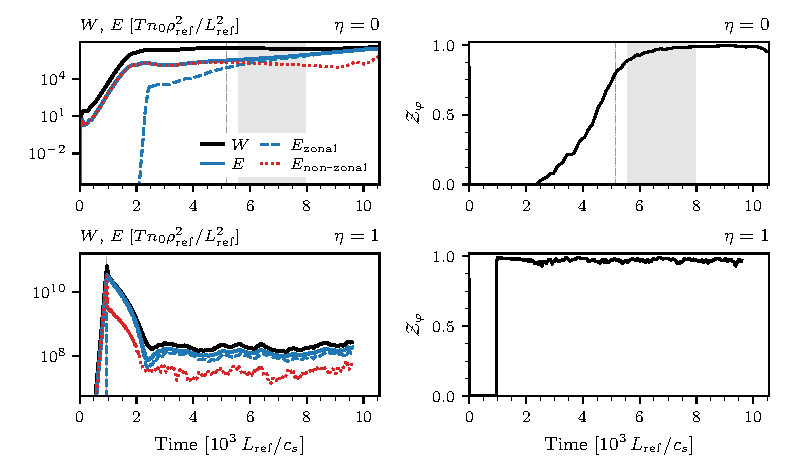
\includegraphics[width=\textwidth]{plots/dipole_NL_fig4.pdf}
\caption{Time evolution in the dipole at $c_\mathrm{surf} = 1.10$, in the layout of \Cref{fig:nonlinear_monitor} and in the radially elongated box of \cref{app:aspect}. \textit{Top row:} $\eta = 0$, $\omega_n = 2$. \textit{Bottom row:} $\eta = 1$, $\omega_n = \omega_T = 2$. \textit{Left column:} free energy $W(t)$ (black), electrostatic energy $E(t)$ (blue solid), and $E$ split into zonal ($k_y = 0$, blue dashed) and non-zonal ($k_y > 0$, red dotted) parts. \textit{Right column:} the zonal fraction $\mathcal{Z}_\varphi$ of \cref{eq:zonal_fraction}. The dotted vertical line marks the zonal lock, when $\mathcal{Z}_\varphi$ first reaches $0.8$ and stays there. The shaded band in the $\eta = 0$ row is the averaging window shared by \Cref{fig:dipole_spectral_flux,fig:parallel_leg,fig:pitch_entropy}. Each row is drawn over its full simulation, on a common time axis.}
\label{fig:dipole_NL_fig4}
\end{figure}

\Cref{fig:dipole_spectral_flux} shows $\Pi_E$ (left-hand side) and $\Pi_Z$ (right-hand side) for the $\eta = 0$ dipole run. The fluxes time-averaged the shaded region in \Cref{fig:dipole_NL_fig4}). The condensate is still strengthening across the window with the zonal part of $E$ growing more than fivefold. In the dipole the measured $\hat E$ of \cref{eq:GK_W_E_defs} keeps only the Debye-screening part of the electrostatic energy: the bounce-average residue $\langle\phi^2\rangle - \langle\bar\phi^2\rangle$ that \cref{eq:elec_energy} also carries [and which vanishes identically in the $Z$-pinch] is not included. This is anticipated to be a small correction over the transfer band where the screening term dominates. The two invariants are again transferred in opposite directions. The spectral flux of electrostatic energy $\Pi_E$ is negative across the long-wavelength range. The spectral flux of free energy $\Pi_Z$ is positive from the injection scale onwards. The dual cascade therefore operates in dipole geometry as expected.

\begin{figure}
\centering
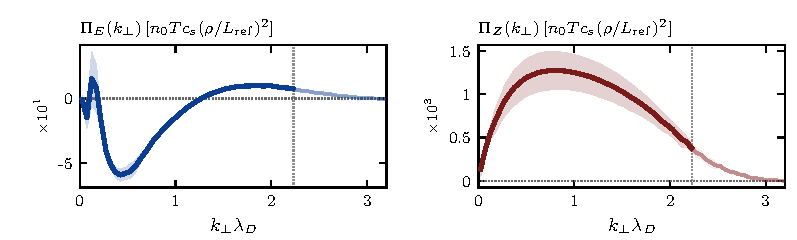
\includegraphics{plots/dipole_spectral_flux.pdf}
\caption{Cumulative spectral fluxes of \cref{eq:Pi_def} in the dipole at $c_\mathrm{surf} = 1.10$ ($\eta = 0$, $\omega_n = 2$), as in \Cref{fig:direct_cascade_flux} for the $Z$-pinch. \textit{Left:} $\Pi_E(\kperp)$. \textit{Right:} $\Pi_Z(\kperp)$. Averaged over the saturated window $t \approx 5600$--$8000\,L_\mathrm{ref}/c_s$, entirely after the zonal lock (the shaded window of \Cref{fig:dipole_NL_fig4}). Shaded bands: scatter in one standard deviation. Curves are drawn solid to the largest complete $\kperp$ shell (dotted vertical) and faded beyond it, where the rectangular box no longer contains every mode of a shell and the curve is only a partial-shell estimate.}
\label{fig:dipole_spectral_flux}
\end{figure}



Again the fluid interchange driven turbulence that carries large-scale vortices. \Cref{fig:dipole_morph} shows the evolution of the equatorial normalised potential $\varphi(x, y)$ at $\eta = 0$ (left-hand column) and $\eta = 1$ (right-hand column). Formation follows the $Z$-pinch sequence (\Cref{fig:phi_chi_snap}); the streamers first go unstable to the secondary instability before giving way to the zonal condensate whose rise \Cref{fig:dipole_NL_fig4} tracks. The columns differ in what survives within the condensate. At $\eta = 0$ the developed state is a set of clean zonal bands. At $\eta = 1$ coherent vortex cores remain embedded in the bands [gold dashed contours] as in the $Z$-pinch.

\begin{figure}
\centering
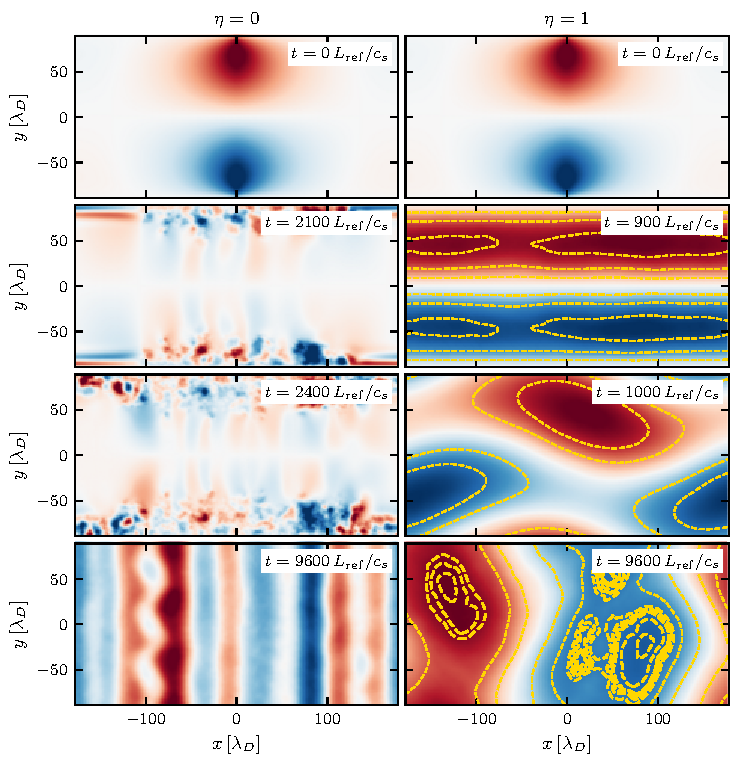
\includegraphics{plots/dipole_morph_evolution.pdf}
\caption{Formation of the dipole state at the $z = 0$ equator: potential $\varphi(x, y)$ at $c_\mathrm{surf} = 1.10$ in the radially elongated box of \cref{app:aspect} ($2\!:\!1$ in $x\!:\!y$). \textit{Left column:} $\eta = 0$, $\omega_n = 2$. \textit{Right column:} $\eta = 1$, $\omega_n = \omega_T = 2$. Rows, top to bottom: close to the initial condition, formation of streamers, the secondary instability, the developed state. Colour scales saturate at the 99th percentile of each panel, and gold dashed contours on the $\eta = 1$ column mark fixed fractions of each panel's colour scale, as in \Cref{fig:phi_chi_snap}.}
\label{fig:dipole_morph}
\end{figure}


\subsection{Fine-scale structure from nonlinear phase mixing}\label{sec:dipole_phasemix}

It was argued that nonlinear phase mixing in closed-field-line geometry with varying $|\bB|$ should build structure across $(\psi,\alpha,l,\lambda)$ (\cref{sec:theory}). The forward $W$ cascade should excite higher $\kperp$ and smaller scales in $l$, and the bounce average over $B(l)$ couples that parallel structure to pitch angle. We can \textcolor{red}{observe} signatures of both legs directly in the dipole simulations.

Since $|\bB|$ varies along the field line and this generates parallel structure in the free energy, the forward cascade can now exit through a parallel sink as well as through velocity space. The constant-$|\bB|$ $Z$-pinch has no such channel and removes the free energy in velocity space alone. \Cref{fig:parallel_leg} shows the cumulative share of the removal carried by each sink as a function of $\kperp$; results are shown for the $Z$-pinch (left-hand side) for the dipole (right-hand side). In the $Z$-pinch the velocity-space sink $\varepsilon_v$ accounts for all of the injected free energy. In the dipole the parallel sink $\varepsilon_\parallel$ carries roughly a third. That share is not stationary within the averaging window and weakens as the condensate locks. 

\begin{figure}
\centering
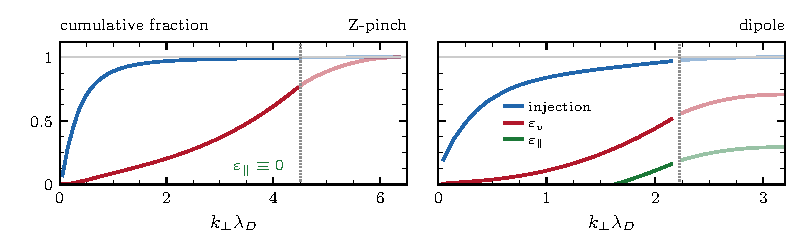
\includegraphics{plots/parallel_leg.pdf}
\caption{Cumulative $\kperp$ removal of the free energy by channel at the $\eta = 0$, $\omega_n = 2$ drive: the velocity-space sink $\varepsilon_v$ and the parallel sink $\varepsilon_\parallel$ as fractions of the total removal, with the injection spectrum for reference. \textit{Left:} $Z$-pinch, averaged over $t = 20\,000$--$25\,000\,L_\mathrm{ref}/c_s$. \textit{Right:} dipole at $c_\mathrm{surf} = 1.10$, averaged over $t = 5600$--$8000\,L_\mathrm{ref}/c_s$. Complete $\kperp$ shells are drawn solid to the dotted line. Beyond it the rectangular box no longer contains every mode of a shell and the faded curves are only partial-shell estimates.}
\label{fig:parallel_leg}
\end{figure}

The pitch-angle structure and its associated phase mixing can be visualised with the help of passive tracers. \Cref{fig:lambda_phase_mixing_3d} makes this pitch-angle decorrelation visible. Tracers are launched from a single point (star) and each tracer is advected by its own bounce-averaged potential, \cref{eq:orbit_avg} applied to $\phi$ at fixed drift-plane position:
\begin{equation}\label{eq:phibar_tracer}
\bar\phi(x, y; \lambda, t) \;=\; \frac{1}{\hat\tau(\lambda)}\int_{l_1}^{l_2}\!\frac{\phi(x, y, l, t)\,\rmd l}{\sqrt{1 - \lambda B(l)}},
\end{equation}
with $\phi$ taken from a $Z$-pinch (left-hand side) and a dipole (right-hand side) simulation, each in its saturated phase. Pitch angle enters only through the averaging window in \cref{eq:phibar_tracer}. A deeply trapped particle samples $\phi$ near the equator alone, whereas a passing particle averages along the whole line. Particles of different pitch therefore undergo distinct $\vE \times \vB$ motion in the drift plane. Stacked by pitch angle, the tracers launch as a vertical filament; one trajectory per pitch angle. A flute-like $\phi$ is independent of $l$, so every pitch angle sees the same $\bar\phi$ and the filament remains intact however turbulent the drift plane ($Z$-pinch, left-hand side). In the dipole the filament is sheared apart (right-hand side). The difference is the $l$-structured part of $\phi$ built by the forward cascade and read through the orbit average. See also figure~1 of \citet{Plunk2012}.

\Cref{fig:pitch_entropy} resolves each invariant in pitch angle in the saturated state. The left-hand panel carries the electrostatic energy,
\begin{equation}\label{eq:E_lambda}
E(\lambda) \;=\; \sum_{\mathbf{k}_\perp} \bigl|\bar\phi_{\mathbf{k}_\perp}(\lambda)\bigr|^2,
\end{equation}
the bounce average of \cref{eq:phibar_tracer} applied mode by mode and summed over the perpendicular spectrum. The spectrum $E(\lambda)$ is flat to $3\%$ across the full range, and to $10\%$ for the non-zonal part alone. A flute-like $\phi$ would make $E(\lambda)$ exactly flat and so the residual variation measures how completely the $\lambda$-independent state has been realised. This is prediction (ii): the inverse cascade terminates in low-$\kperp$, nearly $\lambda$-independent modes, which are consequently also nearly $l$-independent. The right-hand panel applies the same resolution to the entropy,
\begin{equation}\label{eq:Z_lambda}
Z(\lambda) \;=\; \frac{1}{\mathcal{D}(\lambda)}\sum_a \int \rmd k_x\, \rmd k_y \oint \frac{\rmd l}{B}\int \rmd^3\bv\; \delta\!\bigl(\lambda - \lambda(\bv, l)\bigr)\, \frac{T_a\,\bigl|\hat g_a\bigr|^2}{2\, f_{a0}},
\end{equation}
the entropy density averaged over the constant-$\lambda$ surface in phase space, in which
\begin{equation}\label{eq:dos}
\mathcal{D}(\lambda) \;=\; \sum_a \oint \frac{\rmd l}{B}\int \rmd^3\bv\; \delta\!\bigl(\lambda - \lambda(\bv, l)\bigr)
\end{equation}
is the phase-space density of states. Dividing by $\mathcal{D}$ removes its divergence at the separatrix. The spectrum $Z(\lambda)$ varies across the range. It is largest in the passing region, with the maximum well away from the deeply passing limit $\lambda \to 0$, falls to a minimum near the separatrix $\lambda = 1/B_\mathrm{max}$, and recovers part of the way back over the trapped range. This is prediction (iii): varying $|\bB|$ opens a pitch-angle channel that is closed at constant $|\bB|$, and the saturated free energy is structured in $\lambda$. The theory predicts that the structure exists, not what form it takes. Together the two panels of \Cref{fig:pitch_entropy} show the two legs of the phase-space cascade of \cref{sec:lambda_coupling} directly; one invariant flowing to pitch-angle-independent modes and the other developing pitch-angle structure.



\begin{figure}
\centering
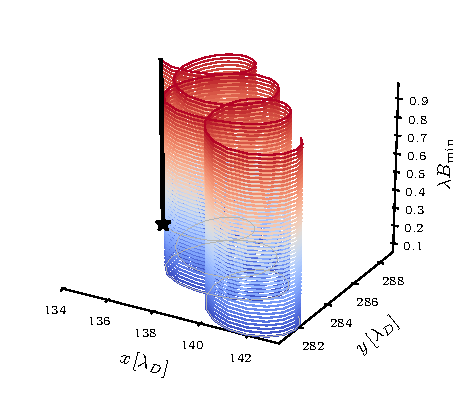
\includegraphics[width=0.49\textwidth]{plots/zpinch_lambda_phase_mixing_3d.pdf}\hfill
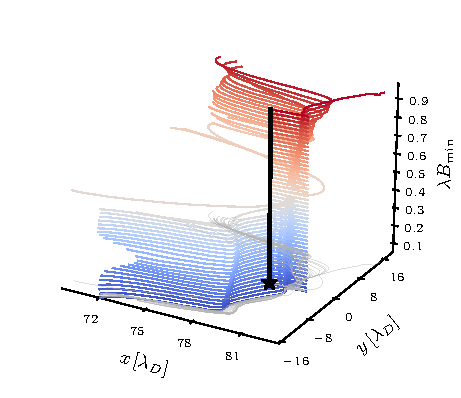
\includegraphics[width=0.49\textwidth]{plots/dipole_lambda_phase_mixing_3d.pdf}
\caption{Passive tracers launched from one point (star), each advected by its own bounce-averaged potential $\bar\phi(\lambda)$, \cref{eq:phibar_tracer}, and stacked at its pitch angle $\lambda B_\mathrm{min}$: the bundle launches as a vertical filament, one trajectory per pitch angle. \textit{Left:} $Z$-pinch. \textit{Right:} dipole.}
\label{fig:lambda_phase_mixing_3d}
\end{figure}

\begin{figure}
\centering
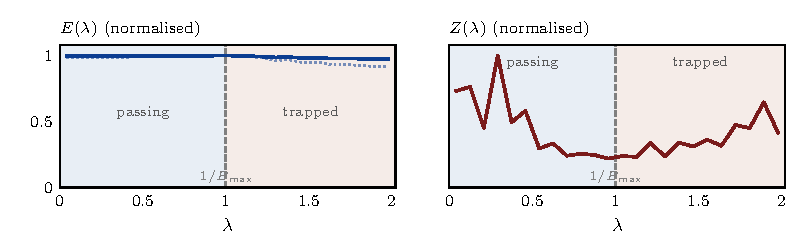
\includegraphics{plots/pitch_entropy.pdf}
\caption{Pitch-angle structure of the two invariants in the saturated dipole at $c_\mathrm{surf} = 1.10$ ($\eta = 0$, $\omega_n = 2$), in the layout of \Cref{fig:direct_cascade_flux}. \textit{Left:} the pitch-angle-resolved electrostatic energy $E(\lambda)$ of \cref{eq:E_lambda}, with its non-zonal part dotted. \textit{Right:} the pitch-angle entropy $Z(\lambda)$ of \cref{eq:Z_lambda}, averaged over six snapshots within $t = 5600$--$8000\,L_\mathrm{ref}/c_s$, the shaded window of \Cref{fig:dipole_NL_fig4}. The $E(\lambda)$ average spans the same window. Passing ($\lambda < 1/B_\mathrm{max}$) and trapped ($\lambda > 1/B_\mathrm{max}$) regions are shaded, the vertical dashed line marks the separatrix, and both curves are normalised to their maxima.}
\label{fig:pitch_entropy}
\end{figure}



\section{Discussion and conclusions}\label{sec:conclusions}

We have studied the nonlinear saturation of electron--positron plasma turbulence in the simple closed-field-line geometries relevant to planned pair-plasma experiments. In the experimentally relevant ordering $\rho \ll \lambdaD \ll L$, the dynamics conserve two quadratic invariants: the electrostatic energy $E$ and the free energy $W$. Their simultaneous conservation leads, through the Fj\o rtoft argument \citep{Fjortoft1953}, to a dual cascade. The electrostatic energy is transferred inversely to perpendicular scales larger than the Debye length, while the free energy is transferred forward to fine scales in phase space. Nonlinear gyrokinetic simulations with \gene\ \citep{Jenko2000} support this picture in both the $Z$-pinch and the levitated dipole. At large scales, the inverse transfer is channelled into zonal ($k_y=0$) modes. These are neither driven by the instability nor, in the absence of geodesic curvature, subject to collisionless damping. With no intrinsic intermediate scale available to arrest the transfer, the electrostatic energy condenses at the largest accessible scale---the box scale in our simulations (\cref{app:aspect}) and, potentially, the device scale in an experiment. Magnetic-field-strength variation modifies the forward cascade without changing this basic nonlinear organisation. In the dipole, $W$ is transferred both to small perpendicular scales and into the parallel direction. As it does so, it develops increasingly fine pitch-angle structure. The inverse transfer of $E$ instead approaches the flute state described in \cref{sec:fjortoft_general}, from which the large-scale condensate is assembled.

As the drive is increased through either linear threshold, the plasma settles into a nearly coherent zonal-flow-dominated state. The instability is strongly suppressed and only weak residual fluctuations remain. Below both linear thresholds we find no evidence of subcritical excitation. The free energy relaxes to the numerical noise floor, far below the available-energy bound of \citet{Helander2017}, and the plasma is effectively turbulence-free. Above threshold, transport saturates at a small residual level sufficient to sustain the forward free-energy cascade. Both particle and heat fluxes remain well below the mixing-length estimate for Debye-scale eddies turning over on the $L/\vth$ timescale. The heat flux is smaller by roughly three orders of magnitude, while the particle flux reverses sign at sufficiently strong drive. Our simulations bracket the quasilinear reversal predicted by \citet{HelanderConnor2016}.

\textcolor{red}{What sets that residual level is the dissipation. The gradients are the only source of free energy in these simulations and the velocity-space sink the only irreversible channel, so a steady state requires the sink to remove free energy as fast as the gradients supply it, and that requirement pins a finite gradient-weighted combination of the fluxes \cref{eq:W_balance}. Neither drive admits a floor without dissipation. The injection that has to be matched is itself a small residue of a much larger exchange: the gradients hand free energy to the fluctuations and take most of it back, the turbulence retaining about half of the exchange at the weaker drive and a few parts in a thousand at the stronger, while the transfer between modes is larger still and cancels over the spectrum rather than in time. Only the residue is dissipated. Resolved in binormal wavenumber the floor is a flow rather than a balance struck at any one scale, free energy entering at long wavelength and leaving at short, with the zonal modes standing outside it, holding most of both invariants and taking no drive. The strongly driven run has not reached that balance. It is still draining the store its saturation burst left, at the rate the drift resonance can deliver free energy to the velocity-space scales the sink reaches, and the state it is heading for carries a dissipation floor and a transport floor of the kind the weakly driven run already sits at.}

Low-transport states of this kind are familiar from electron--ion turbulence in closed-field-line geometry \citep{Kobayashi2009,KobayashiRogers2012,BanonNavarro2016}, from vortex-dominated models of ETG turbulence \citep{Nakata2010}, and from the Dimits-shift regime \citep{Dimits2000,KobayashiRogers2012}. In those systems the zonally regulated state generally survives only over a finite range of driving gradients. A tertiary instability then restores strong transport. Here, by contrast, the zonal-locked state persists throughout the full range of drives simulated. The finite-Larmor-radius mechanism responsible for the tertiary instability in the electron--ion problem lies outside the present ordering because the condensate resides at $\kperp\rho\ll1$. The constant-$|\bB|$ $Z$-pinch also admits no phase mixing in pitch angle, the bounce-average counterpart of that finite-Larmor-radius mechanism, because no particle is trapped and the orbit-averaged potential $\bar\phi$ is the same for every pitch angle (\cref{sec:lambda_coupling}). A pair-plasma tertiary instability at finite $\kperp\rho$ in dipole geometry is therefore not excluded, but lies beyond the scope of the present work.

The dual-cascade constraint itself is not specific to pair plasmas. The same two-invariant structure arises in electron--ion plasmas at frequencies below the ion bounce frequency. In that regime, the large-scale trapped-ion mode can be regulated by nonlinear coupling to a distinct population of shorter-scale modes \citep{Kingsbury1994}. That particular saturation route is unavailable here because the corresponding small-scale modes of the pair plasma are linearly stable \citep{Helander2014}. The essential consequence of pair symmetry instead enters through the field equation of \cref{sec:polarisation}. With both species treated kinetically and no adiabatic response, Debye shielding provides the only remaining polarisation term. The relevant polarisation scale is therefore $\lambdaD$ rather than the Larmor radius. The instability that feeds the turbulence is itself a finite-Debye-length effect. In the strict limit $\kperp\lambdaD\to0$, no microinstability exists \citep{Helander2014}. The residual interchange drive appears only through the finite correction $\kperp^2\lambdaD^2$. Once excited, however, the turbulence is organised by the same two quadratic invariants. The electrostatic energy is transferred inversely beyond the Debye scale, while the free energy is transferred forward through phase space. Geometry then determines the directions available to that forward transfer: $\kperp$ alone in the constant-$|\bB|$ $Z$-pinch, and both $\kperp$ and pitch angle $\lambda$ in the dipole.



In summary, our results imply a strong suppression of turbulence via an inverse cascade in the four-dimensional phase space $(\psi, \alpha, l, \lambda)$. This bodes well for the magnetic confinement of pair plasmas in closed-field-line geometry. Once formed, the condensate decays only by classical collisional diffusion, which is exceedingly small when $\kperp\sim 1/\lambdaD$ and $\rho\ll\lambdaD$, so the low-transport state is long-lived. A dilute pair plasma close to marginality is a quiet system, and where its profiles are free to evolve the transport should relax them towards the linearly stable region, making it quieter still. Whether the locked state is reachable in stellarator geometry, in the regimes accessible to APEX and EPOS \citep{Pedersen2012, Stoneking2020}, is left to future work, as is the rational surface of a tokamak or stellarator, which closes the field lines but carries the finite geodesic curvature that would undo the strict zonal-flow protection found here.


\section*{Acknowledgements}
\textcolor{red}{The authors would like to thank J.~Ball, R.~Nies, A.~A.~Schekochihin, and W.~Clarke for helpful discussions and suggestions at various stages of this project.} Part of this work was performed using resources provided on the PITAGORA supercomputer of the National Supercomputing Consortium CINECA, under the project GEMST26.

\section*{Funding}
The authors received no specific funding for this work.

\section*{Declaration of interests}
The authors report no conflict of interest.

\section*{Data availability statement}
The data that support the findings of this study are available from the corresponding author on reasonable request.

\appendix
\section{The strongly-driven fluid limit}\label{app:fluid}

For $Z$-pinch geometry, in the strongly-driven limit the drift-kinetic system \cref{eq:dke}--\cref{eq:poisson} closes into a two-field fluid model. This appendix derives that model, referred to throughout the main text, and maps it onto the interchange system of \citet{ClarkeUnpub}. The derivation takes two velocity moments of the drift-kinetic equation. The first is the charge, which Poisson's equation ties to the potential and which yields a vorticity equation. The second is a pressure-like moment, which the magnetic drift couples to the first and which yields an advection equation of its own. The strongly-driven ordering closes the pair.

\subsection{From the drift-kinetic equation to the two-field model}\label{sec:app_fluid_derivation}

In the $Z$-pinch $|\bB|$ is constant along the closed field line, so the orbit average \cref{eq:orbit_avg} is a simple line average and $\bar\phi = \phi$ for every particle, the Larmor-radius dependence having already been removed by the ordering \cref{eq:ordering}. The potential a particle feels therefore does not depend on its energy or its pitch angle, and every particle is advected by the same flow,
\begin{equation}\label{eq:app_fluid_vE}
\vec{v}_E \;=\; \uvec{b}\times\grad\phi/B .
\end{equation}
In the slab coordinates $(x, y) = (\psi, \alpha)$ the drift-kinetic equation \cref{eq:dke} reads
\begin{equation}\label{eq:app_fluid_dke}
\frac{\partial h_a}{\partial t} \;+\; \vec{v}_E\bcdot\grad h_a \;+\; \hat{v}_{da}\,u(\bv)\,\frac{\partial h_a}{\partial y}
\;=\; \frac{e_a}{T}\,f_{a0}\left(\frac{\partial \phi}{\partial t} \;-\; v_{*a}^T\,\frac{\partial \phi}{\partial y}\right),
\end{equation}
closed by Poisson's equation \cref{eq:poisson}. Here $u(\bv)$ is the magnetic drift \cref{eq:vd} in units of its thermal value,
\begin{equation}\label{eq:app_fluid_u}
u(\bv) \;\equiv\; \frac{\vpar^2 + \tfrac{1}{2}\vperp^2}{\vth^2} ,
\qquad
\vth \;\equiv\; \sqrt{\frac{2T}{m}} ,
\end{equation}
and $\langle\,\cdot\,\rangle_\bv$ denotes the Maxwellian velocity average,
\begin{equation}\label{eq:app_fluid_vavg}
\bigl\langle A \bigr\rangle_\bv \;\equiv\; \frac{1}{n_0}\int \rmd^3\bv\; A(\bv)\, f_{a0}(\bv) ,
\qquad\text{so that}\qquad
\bigl\langle u \bigr\rangle_\bv \;=\; 1 .
\end{equation}
The coefficient $v_{*a}^T$ is the diamagnetic drive of \cref{eq:vstar}. The species drift coefficients are
\begin{equation}\label{eq:app_fluid_vd_species}
\hat{v}_{dp} \;=\; -\hat{v}_{de} \;\equiv\; -\hat{v}_d ,
\qquad
\hat{v}_d \;=\; \frac{2T}{eBR} \;>\; 0 ,
\qquad
k_y \hat{v}_d \;=\; \hat\omega_d
\end{equation}
(\Cref{tab:norms}), the positrons taking the negative sign, which is that of \cref{eq:vd} at the destabilising curvature.

That common advecting flow is what closes the moment hierarchy. Because the flow is the same for every particle it passes through the velocity integral,
\begin{equation}\label{eq:app_fluid_factorise}
\int \rmd^3\bv\; w(\bv)\,\vec{v}_E\bcdot\grad h_a \;=\; \vec{v}_E\bcdot\grad \int \rmd^3\bv\; w(\bv)\,h_a ,
\end{equation}
for any weight $w(\bv)$, so the nonlinearity couples no velocity moments and there is no nonlinear phase mixing \citep{Dorland1993}. The only coupling left between moments is linear, through the factor $u(\bv)$ in the drift term, and that coupling is weak in the strongly-driven ordering
\begin{equation}\label{eq:app_fluid_ordering}
\hat\omega_d \;\ll\; \omega \;\ll\; \omega_* ,
\end{equation}
which is the regime of the fluid branch of \cref{sec:linear}, where the growth rate is the geometric mean of drive and drift at $\kperp\lambdaD \sim 1$ \cref{eq:gamma_scaleinv_pre}. The closure problem is therefore purely linear and the ordering alone closes it, whereas gyrofluid models must truncate both the linear and the nonlinear mixing by hand \citep{Dorland1993}. What the ordering discards is the kinetic character of the drift: expanding the resonance in $\hat\omega_d/\omega$ removes its pole, so the closure keeps the interchange drive and gives up the Landau damping carried by the energy dependence of the drift. The hierarchy then closes after two moments, and we take them in turn.

The first moment is the charge. In a pair plasma the charge density is $e(n_p - n_e)$, so that moment is the difference of the two species, and we take $1/(2n_0)$ times the velocity integral of the difference of \cref{eq:app_fluid_dke}, positrons minus electrons. Two things happen at once. The diamagnetic drive cancels, because it enters each species multiplied by $e_a$ while $v_{*a}^T$ carries a compensating $1/e_a$, so both species carry the same coefficient $e_a v_{*a}^T$ \cref{eq:vstar} and the difference annihilates it. The drift term, in contrast, survives, and brings in the $u$-weighted, species-summed moment
\begin{equation}\label{eq:app_fluid_chi_def}
\chi \;\equiv\; \frac{1}{2 n_0} \int \rmd^3\bv\; u(\bv)\,\bigl(h_p + h_e\bigr).
\end{equation}
Poisson's equation then converts the charge moment into $(1 - \lambdaD^2\grad_\perp^2)\,\hat\phi$, with $\hat\phi \equiv e\phi/T$, the unit term being the adiabatic part of $\delta f$ \cref{eq:df_split} and the Laplacian the Debye polarisation, and the charge moment reads
\begin{equation}\label{eq:app_fluid_charge_moment}
\frac{\partial}{\partial t}\Bigl[\bigl(1 - \lambdaD^2\grad_\perp^2\bigr)\hat\phi\Bigr]
\;+\; \vec{v}_E\bcdot\grad\Bigl[\bigl(1 - \lambdaD^2\grad_\perp^2\bigr)\hat\phi\Bigr]
\;-\; \hat{v}_d\,\frac{\partial \chi}{\partial y}
\;=\; \frac{\partial \hat\phi}{\partial t}.
\end{equation}
The Boltzmann part of the response now cancels identically. Its time derivative cancels the $\partial_t\hat\phi$ source on the right of \cref{eq:app_fluid_charge_moment}, and its advection vanishes by antisymmetry of the bracket,
\begin{equation}\label{eq:app_fluid_antisym}
\vec{v}_E\bcdot\grad\hat\phi \;\propto\; \pbra{\hat\phi}{\hat\phi} \;=\; 0 .
\end{equation}
Neither step invokes the ordering, so for the symmetric pair plasma the cancellation is exact. What survives is the vorticity equation
\begin{equation}\label{eq:app_fluid_vort_dim}
\frac{\partial}{\partial t}\bigl(-\lambdaD^2\,\grad_\perp^2\,\hat\phi\bigr) \;+\; \vec{v}_E\bcdot\grad\bigl(-\lambdaD^2\,\grad_\perp^2\,\hat\phi\bigr) \;=\; \hat{v}_d\,\frac{\partial \chi}{\partial y}.
\end{equation}
whose polarisation is the pure Laplacian. This is a structural difference from the standard drift-wave models. In the Hasegawa--Mima and cold-ion-temperature-gradient equations the retained adiabatic response of the second species produces the operator $(1 - \grad_\perp^2)$ \citep{HasegawaMima1978}, whereas here neither species is adiabatic: each species' adiabatic response is cancelled by its own $\partial_t\phi$ drive, so the unit term is absent at every wavenumber. The formally small coefficient $\hat{v}_d$ survives on the right of \cref{eq:app_fluid_vort_dim} only because $\chi$ is correspondingly large,
\begin{equation}\label{eq:app_fluid_chi_large}
\chi \;\sim\; \left(\frac{\omega_*}{\hat\omega_d}\right)^{1/2} \hat\phi ,
\end{equation}
as the normalisation of \Cref{tab:plunk_norms} shows. After normalisation the two fields are of the same order.

The second moment is $\chi$ itself, and we obtain its equation by weighting \cref{eq:app_fluid_dke} with $u(\bv)$ and summing over species. This time the $\partial_t\phi$ source cancels, being odd in $e_a$, while the diamagnetic drive survives. The drive $v_{*a}^T$ of \cref{eq:vstar} carries a density-gradient part and a temperature-gradient part, and the $u$ weight integrates them separately. Both integrals are unity,
\begin{equation}\label{eq:app_fluid_maxwellian}
\bigl\langle u \bigr\rangle_\bv \;=\; \left\langle u\left(\frac{m v^2}{2T} - \frac{3}{2}\right)\right\rangle_\bv \;=\; 1 ,
\end{equation}
so the two gradients enter only through their sum, the combination $(1+\eta)\,v_*$ with $v_* = T/(e B L_n)$ the slab form of \cref{eq:vstar}. This gives
\begin{equation}\label{eq:app_fluid_chi_dim}
\frac{\partial \chi}{\partial t} \;+\; \vec{v}_E\bcdot\grad\chi \;=\; -(1+\eta)\,v_*\,\frac{\partial \hat\phi}{\partial y}.
\end{equation}
but only after one term has been dropped. The drift term also couples $\chi$ to the $u^2$-weighted difference moment
\begin{equation}\label{eq:app_fluid_xi_def}
\xi \;\equiv\; \frac{1}{2 n_0}\int \rmd^3\bv\; u^2(\bv)\,\bigl(h_p - h_e\bigr),
\end{equation}
which enters the left-hand side of the $\chi$ equation as $-\hat{v}_d\,\partial\xi/\partial y$. Unlike $\chi$, the moment $\xi$ is not amplified by the drive, and in the strongly-driven linear response it is $\order{\hat\phi}$, so that term is smaller than the retained drive on the right-hand side of \cref{eq:app_fluid_chi_dim} viz
\begin{equation}\label{eq:app_fluid_xi_small}
\frac{\hat{v}_d\,\partial_y \xi}{(1+\eta)\,v_*\,\partial_y \hat\phi} \;=\; \order{\frac{\hat\omega_d}{\omega_*}} .
\end{equation}
We discard it in \cref{eq:app_fluid_chi_dim}. This is the single point at which the hierarchy is cut.

\subsection{Normalisation and the scale-invariant rate}\label{sec:app_fluid_norm}

Both equations still carry the drives as coefficients, and one choice of units removes them. We measure lengths in $\lambdaD$ and time in the interchange time,
\begin{equation}\label{eq:app_fluid_tau}
\tau \;\equiv\; \frac{\lambdaD\sqrt{R L_*}}{\vth\,\rho} ,
\qquad
\frac{1}{L_*} \;\equiv\; \frac{1}{L_n} + \frac{1}{L_T} ,
\qquad
\eta \;=\; \frac{L_n}{L_T} ,
\end{equation}
whose inverse is the geometric mean of drive and drift and so the interchange rate at $\kperp\lambdaD \sim 1$ \cref{eq:gamma_scaleinv_pre}; $\rho$ is the Larmor radius of \cref{eq:ordering}. We then rescale the fields as,
\begin{equation}\label{eq:app_fluid_units}
\varphi \;\equiv\; \frac{e\phi}{T}\,\frac{\sqrt{R L_*/2}}{\lambdaD},
\qquad
\chi \;\to\; \frac{L_*}{\lambdaD}\,\chi .
\end{equation}
and the pair \cref{eq:app_fluid_vort_dim} and \cref{eq:app_fluid_chi_dim} becomes the parameter-free system
\begin{align}
\frac{\partial}{\partial t}\bigl(-\grad_\perp^2\,\varphi\bigr) \;+\; \pbra{\varphi}{-\grad_\perp^2\,\varphi} \;&=\; \frac{\partial \chi}{\partial y}, \label{eq:app_fluid_vort}\\
\frac{\partial \chi}{\partial t} \;+\; \pbra{\varphi}{\chi} \;&=\; -\frac{\partial \varphi}{\partial y}, \label{eq:app_fluid_chi}
\end{align}
with the Poisson bracket
\begin{equation}\label{eq:app_fluid_bracket}
\pbra{A}{B} \;=\; \frac{\partial A}{\partial x}\frac{\partial B}{\partial y} \;-\; \frac{\partial A}{\partial y}\frac{\partial B}{\partial x} .
\end{equation}
\Cref{tab:plunk_norms} collects the normalisations. The drives have gone into the units, and the gradient ratio $\eta$ into $L_*$.

\begin{table}
\centering
\renewcommand{\arraystretch}{1.2}
\begin{tabular}{lcl}
\hline
Quantity & Dimensionless symbol & Definition \\
\hline
Perpendicular coordinate    & $x, y$       & $x_\mathrm{phys}/\lambdaD$ \\
Time                        & $t$          & $t_\mathrm{phys}\cdot \vth\,\rho/(\lambdaD\sqrt{R L_*})$ \\
Potential                   & $\varphi$    & $(e\phi/T) \cdot \sqrt{R L_*/2}\,/\lambdaD$ \\
Pressure-like field         & $\chi$       & $\chi_\mathrm{phys}\cdot L_*/\lambdaD$ \\
\hline
Effective gradient          & $L_*^{-1}$   & $L_n^{-1} + L_T^{-1}$ \\
Drive ratio                 & $\eta$       & $L_n/L_T$, absorbed in $L_*$ \\
\hline
\end{tabular}
\caption{Normalisation of the strongly-driven $Z$-pinch two-field fluid model \cref{eq:app_fluid_vort} and \cref{eq:app_fluid_chi}. The pressure-like field $\chi_\mathrm{phys}$ is defined in \cref{eq:app_fluid_chi_def}.}
\label{tab:plunk_norms}
\end{table}

The pair that remains has no perpendicular scale of its own. It is invariant under
\begin{equation}\label{eq:app_fluid_rescale}
(x, y) \;\to\; (x, y)/c ,
\qquad
\varphi \;\to\; \varphi/c^2 ,
\qquad
\chi \;\to\; \chi/c ,
\end{equation}
which is the real-space form of the invariance of \cref{eq:gamma_scaleinv} under $\vk \to c\,\vk$. Linearising about rest, with $\varphi$ and $\chi$ varying as $\exp(\mathrm{i}\vk\bcdot\vec{r} - \mathrm{i}\omega t)$, gives
\begin{equation}\label{eq:app_fluid_disp}
\omega^2 \;=\; -\frac{k_y^2}{\kperp^2}
\;\;\Longrightarrow\;\;
\gamma \;=\; \frac{|k_y|}{\kperp},
\end{equation}
in units of $\tau^{-1}$ and with the wavenumbers measured in $\lambdaD^{-1}$. Restoring units,
\begin{equation}\label{eq:app_fluid_disp_dim}
\left(\frac{\gamma}{\hat\omega_d}\right)^{2} \;=\; \frac{\Omega_*(1+\eta)}{(\kperp\lambdaD)^2}
\end{equation}
(\Cref{tab:norms}), which is \cref{eq:gamma_scaleinv_pre} without the offset $-7/4$; that offset enters at the next order in $\hat\omega_d/\omega$, so the two expressions coincide well above the fluid threshold \cref{eq:mph_fluid}. The pair of equations therefore reproduces the scale-independent interchange rate \cref{eq:gamma_scaleinv} and the low-$k_y$ plateau of \Cref{fig:linear_modes}. It inherits no ultraviolet cutoff of its own: the kinetic band is closed by the boundary \cref{eq:mph_kinetic}, at which Debye screening extinguishes the drive, but the rate \cref{eq:app_fluid_disp} is the same at every scale, so any solution of \cref{eq:app_fluid_vort} and \cref{eq:app_fluid_chi} must be supplied with dissipation at small scale.

The threshold \cref{eq:mph_fluid} is what the simulations of this paper are placed against, and they are placed on either side of it. In the $Z$-pinch $\omega_*$ and $\hat\omega_d$ are both proportional to $k_y$, so their ratio is scale-independent and equal to $\Omega_* = \omega_n/2$ exactly (\Cref{tab:norms}). Both runs of \cref{sec:nonlinear} have $\omega_n = 2$ and therefore $\Omega_* = 1$, and the drive combination that the threshold tests is $\Omega_*(1+\eta)$. At $\eta = 0$ that combination is $1$, below the threshold, so the fluid interchange branch does not exist and the turbulence is carried by the kinetic branch, whose growth rate falls with $k_y$ at long wavelength rather than reaching a plateau (\Cref{fig:linear_modes}). At $\eta = 1$ it is $2$, above the threshold, so the fluid branch is present, if not far above onset. The two runs therefore bracket the limit this appendix derives, one on each side, which is what makes the pair of them a test of it. The comparison does not require either run to sit deep in the limit, because the two properties it rests on do not need the ordering: the factorisation \cref{eq:app_fluid_factorise} holds at any drive, and the invariant pair and the directions of its cascades impose no condition on $\Omega_*$. Indeed the transport contrast is largest away from the strongly-driven limit, since at $\omega_* \sim \hat\omega_d$ the drift resonance, which the closure removes, acts at leading order.

\subsection{Relation to a curved-slab interchange system}\label{sec:app_fluid_clarke_sec}

Our fluid model is isomorphic to that used by \citet{ClarkeUnpub} to study interchange-driven turbulence in the reduced-magnetohydrodynamic equations of a curved slab, derived there both from magnetohydrodynamics and from strongly-driven gyrokinetics. Their fields are the velocity and magnetic-flux stream functions $\Phi$ and $\Psi$ together with the buoyancy
\begin{equation}\label{eq:app_fluid_buoyancy}
a \;=\; -\,g\,\frac{\delta\rho}{\rho_0} ,
\end{equation}
driven by the squared Brunt--V\"ais\"al\"a frequency $N^2$. We set $k_z = 0$ and $\Psi = 0$. That restriction defines an exact invariant subspace of their system, and it is also the two-dimensional electrostatic state into which their dynamics collapse below a critical value of their parameter $\Lambda$. Their system then reduces to
\begin{equation}\label{eq:app_fluid_clarke}
\frac{\rmd}{\rmd t}\,\grad_\perp^2\,\Phi \;=\; -\frac{\partial a}{\partial y},
\qquad
\frac{\rmd a}{\rmd t} \;=\; -N^2\,\frac{\partial \Phi}{\partial y},
\qquad
\frac{\rmd}{\rmd t} \;\equiv\; \frac{\partial}{\partial t} + \pbrainline{\Phi}{\cdot}.
\end{equation}
In the units of \Cref{tab:plunk_norms} the substitution $\Phi = \varphi$, $a = \chi$, $N = 1$ turns \cref{eq:app_fluid_clarke} into \cref{eq:app_fluid_vort} and \cref{eq:app_fluid_chi} term by term, so the two systems are isomorphic. The correspondence runs field by field. Their stream function $\Phi$ generates the perpendicular flow, as $\varphi$ generates the $\vE\times\vB$ flow, which here is the whole flow. Their inertia $\grad_\perp^2\Phi$ carries the ion mass density, where ours is the Debye polarisation $-\lambdaD^2\grad_\perp^2\hat\phi$ of \cref{eq:poisson}; both are pure Laplacians. Their buoyancy $a$ corresponds to $\chi$, the pressure-like moment \cref{eq:app_fluid_chi_def}, and their drive to ours through
\begin{equation}\label{eq:app_fluid_N2}
N^2 \;=\; \frac{\hat{v}_d\,(1+\eta)\,v_*}{\lambdaD^2} \;=\; \tau^{-2} ,
\end{equation}
so their time unit $N^{-1}$ is our interchange time $\tau$. Their dispersion relation at $k_z = 0$ gives $\gamma = N\,|k_y|/\kperp$, which is \cref{eq:app_fluid_disp} and hence \cref{eq:gamma_scaleinv}. Neither ideal pair carries a perpendicular scale, and both must be given small-scale dissipation by hand.

The isomorphism is exact for the ideal two-dimensional systems, but the parent systems differ. Theirs is the $k_z = 0$ subspace of a three-field Alfv\'enic system; ours is the strongly-driven limit of the drift-kinetic system \cref{eq:dke}--\cref{eq:poisson}. The drift resonance discarded by the closure is what supplies the sink that the fluid equations lack (\cref{sec:saturation}).


\section{New dipole implementation in \gene\ 3.0+}\label{app:dipole_impl}

This work uses the levitated dipole geometry of \citet{Kennedy2020}. However, its original poloidal-flux implementation becomes ill-conditioned in \gene\ away from the $Z$-pinch limit (\cref{app:dpfix_coords}) and so we adopt instead a length-based field-line coordinate system that keeps every entry of the perpendicular metric $\order{1}$ at every $c_\mathrm{surf}$ and reduces to \gene's standard $Z$-pinch geometry as $c_\mathrm{surf} \to 1$. The dynamical validation is given in \cref{app:theory_compare}.

\subsection{Flux-tube geometry in \gene}\label{app:gene_geom_basics}

\gene\ solves the gyrokinetic equation in a field-aligned local coordinate system $(x, y, z)$ with $x$ radial across flux surfaces, $y$ binormal within a flux surface and perpendicular to $\bB$, and $z$ along the field line. The device geometry enters only through coefficients evaluated on the $z$ grid: the independent metric components $g^{xx}(z), \, g^{xy}(z), \, g^{yy}(z),\, g^{zz}(z)$, the Jacobian $J(z)$, the magnitude $|\bB(z)|$, the radial and parallel derivatives of $|\bB|$, and the curvature drift coefficients. These arrays are built once at initialisation and everything the code needs at every timestep follows from them. In particular, these coefficients are used to construct the perpendicular wavenumber
\begin{equation}
\kperp^2(z) = k_x^2\,g^{xx}(z) + 2 k_x k_y\,g^{xy}(z) + k_y^2\,g^{yy}(z)
\label{eq:kperp_app}
\end{equation}
which enters every gyroaverage and the polarisation density.

As an example, \gene's reference $Z$-pinch module hard-codes
\begin{equation}
g^{xx} = 1, \quad g^{yy} = 1, \quad g^{zz} = (1/R)^2,
\quad J = R, \quad |\bB| = 1
\label{eq:zpinch_metric}
\end{equation}
on every $z$ grid point. The polarisation operator and the SLEPc preconditioner \citep{Roman2010} are tuned for this convention. Both $g^{xx}$ and $g^{yy}$ enter the $\kperp^2$ matrix and the operator is well-conditioned provided they remain $\order{1}$. 

\subsection{The dipole flux tube and $c_\mathrm{surf}$}\label{app:dipole_flux_tube}

Every field line of a single circular ring conductor of radius $r_0$ carrying current $I$ is a closed loop in the poloidal plane that links the ring (see \Cref{fig:dipole_geom_schematic}). The construction has one dimensionless parameter $c_\mathrm{surf}$. The chosen field line crosses the equatorial plane on the outboard side at radius $c_\mathrm{surf}\,r_0$ from the ring centre, a perpendicular distance $\epsilon = (c_\mathrm{surf} - 1)\, r_0$ from the current-carrying coil. We trace the field line once around to find its arc length $L_\mathrm{tube}$ and construct the \gene\ flux tube around it.

As $c_\mathrm{surf} \to 1$, the flux tube is a thin ring just outside the conductor, $|\bB|$ is uniform along its length and the geometry reduces to the $Z$-pinch limit of \cref{eq:zpinch_metric}. Larger values, reaching $c_\mathrm{surf} = 1.4$ in this paper, carry the tube out into a non-circular loop with a magnetic well on the weak-field side. The nonlinear runs of \cref{sec:dipole} use $c_\mathrm{surf} = 1.1$.

\Cref{fig:dipole_metric_csurf} shows the field strength (left-hand side) and the \gene\ Jacobian (right-hand side) along the field line at the six values of $c_\mathrm{surf}$ used in this paper. Both are flat in the $Z$-pinch limit. As $c_\mathrm{surf}$ rises a magnetic well opens at $z = 0$. The field varies by a factor of two along the line at the production value $c_\mathrm{surf} = 1.1$ and by nearly six at $c_\mathrm{surf} = 1.4$. Importantly, the Jacobian stays of order unity throughout by the coordinate choice of \cref{app:dpfix_coords}. As the well deepens, the flute approximation breaks down and trapped-particle dynamics becomes important (\cref{app:convergence} and \cref{app:theory_compare}).

\begin{figure}
\centering
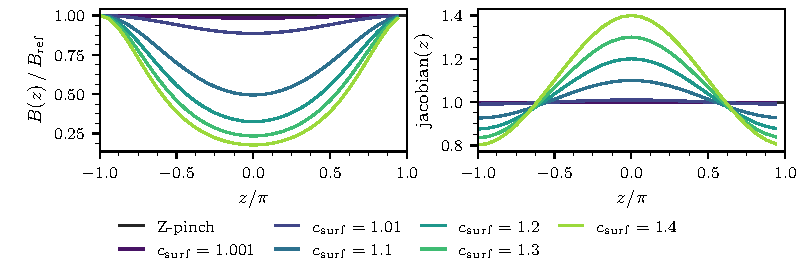
\includegraphics{plots/dipole_metric_csurf.pdf}
\caption{Flux-tube geometry along the closed dipole field line at six values of $c_\mathrm{surf}$. \textit{Left:} parallel profile of $|\bB(z)|/B_\mathrm{ref}$. \textit{Right:} the \gene\ Jacobian along the same line. $z = 0$ is the field minimum and $z = \pm\pi$ is the closest approach to the ring (field maximum). Black horizontal line: $Z$-pinch limit ($c_\mathrm{surf} \to 1$).}
\label{fig:dipole_metric_csurf}
\end{figure}

\subsection{Length-based coordinate convention}\label{app:dpfix_coords}

The dipole geometry was first implemented in \gene\ using the poloidal-flux coordinates of \citet{Kennedy2020}, with the radial coordinate proportional to $\psi$ and hence $g^{xx} = |\grad\psi|^2$. That choice is natural analytically but ill-conditioned in \gene. Since $|\grad\psi| = R\,|\bB|$ follows the field strength, which varies along the loop by a factor of two at the production $c_\mathrm{surf} = 1.10$ and by nearly six at $c_\mathrm{surf} = 1.4$ (\Cref{fig:dipole_metric_csurf}), the metric entries $g^{xx}$ and $g^{yy}$ span orders of magnitude along the line. The $\kperp^2$ matrix of \cref{eq:kperp_app} inherits that range. The polarisation operator and the preconditioner degrade, since both are tuned for the $\order{1}$ entries of \cref{eq:zpinch_metric}. The same choice degrades the parallel grid. Uniform spacing in the flux-based parallel coordinate compresses in arc length by $B_\mathrm{max}/B_\mathrm{min}$ around the loop, so resolution concentrates at the field maxima and little remains in the magnetic well where the particles trap.

The new geometry module instead uses the length-based coordinate system of \Cref{tab:fix_coords}. $L_\mathrm{ref}$ is the natural radius of the closed loop ($L_\mathrm{ref} \to \epsilon$ as $c_\mathrm{surf} \to 1$), and $B_\mathrm{ref}$ is the field strength at the closest approach to the ring, the largest value along the loop. The stored geometry coefficients are
\begin{equation}
g^{xx} = 1, \quad g^{yy} = (R_0/R(z))^2, \quad g^{zz} = 1,
\quad J(z) = R(z)/R_0, \quad |\bB(z)| / B_\mathrm{ref}
\label{eq:fix_metric}
\end{equation}
where $R(z)$ is the cylindrical distance from the ring's axis at parallel position $z$ and $R_0 = r_0$ is the ring radius. The radial and parallel entries are exactly unity at every $c_\mathrm{surf}$, and the others are $\order{1}$, following $R(z)$ and $|\bB(z)|$ along the line. \cref{eq:fix_metric} reduces to \cref{eq:zpinch_metric} term by term as $c_\mathrm{surf} \to 1$, where the $Z$-pinch entries are themselves unity because $R = L_\mathrm{ref}$ there (\Cref{tab:norms}). \Cref{tab:metric_match} tabulates the residual at $c_\mathrm{surf} = 1.001$.

\begin{table}
\centering
\begin{tabular}{cll}
\hline
Coordinate & Definition & Normalisation \\
\hline
$x$ & perpendicular distance to the chosen flux surface & $L_\mathrm{ref}$ \\
$y$ & $R_0 \times$ (toroidal angle) & $L_\mathrm{ref}$ \\
$z$ & arc length along the field line & $L_\mathrm{tube}/(2\pi)$ \\
\hline
\multicolumn{3}{l}{$L_\mathrm{ref} = L_\mathrm{tube}/(2\pi), \qquad B_\mathrm{ref} = \max_z |\bB|$} \\
\hline
\end{tabular}
\caption{Length-based field-line coordinates of the new geometry module and their normalisation.}
\label{tab:fix_coords}
\end{table}

\begin{table}
\centering
\begin{tabular}{lccc}
\hline
Quantity & $Z$-pinch & New module & $\Delta$ \\
\hline
$g^{xx}$    & $1.0$  & $1.000$  & $0$    \\
$g^{yy}$    & $1.0$  & $1.002$  & $+0.2\%$ \\
$g^{zz}$    & $1.0$  & $1.000$  & $0$    \\
$|\bB|$       & $1.0$  & $1.000$  & $0$    \\
$\partial_x \ln |\bB|$  & $-1.0$ & $-1.001$ & $0.1\%$ \\
$J$         & $1.0$  & $0.999$  & $0.1\%$ \\
\hline
\end{tabular}
\caption{Stored geometry coefficients of the new module at $c_\mathrm{surf} = 1.001$ against the \gene\ $Z$-pinch values of \cref{eq:zpinch_metric}.}
\label{tab:metric_match}
\end{table}

\subsection{Linear instability landscape near the production geometry}\label{app:dipole_lin_landscape}

\Cref{fig:dipole_lin_eigenmode_z} shows the parallel structure of the dominant and sub-dominant unstable eigenmodes at $c_\mathrm{surf} = 1.2$. The branch structure continues the $Z$-pinch modes of \cref{sec:linear}; at $\eta = 1$ the two branches collide at the same $k_y\lambdaD \approx 0.14$ as in the $Z$-pinch and continue as a complex-conjugate pair. The dominant modes are flute-like at long wavelength and, as $k_y$ rises, localise towards the field maxima $z = \pm\pi$ and thin in the magnetic well, so trapped and passing particles no longer sample the same potential. The velocity-space counterpart of that departure is shown in \cref{app:convergence}. We verify the new geometry implementation against the bounce-averaged kinetic theory of the dipole dispersion in \cref{app:theory_compare}.

\begin{figure}
\centering
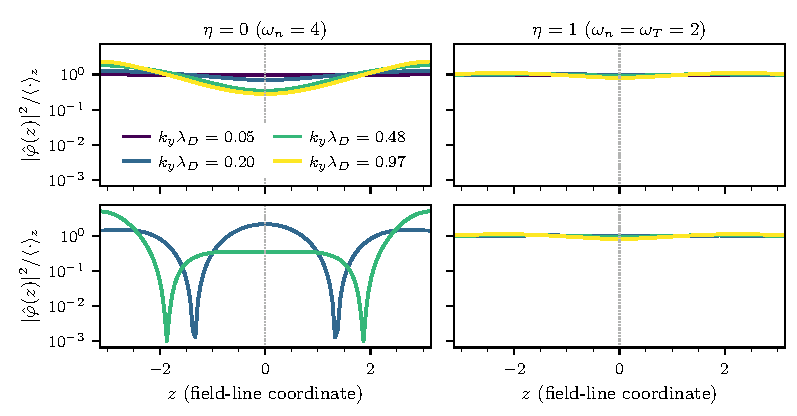
\includegraphics[width=\textwidth]{plots/dipole_linear_eigenmode_z.pdf}
\caption{Parallel structure $|\hat\varphi(z)|^2$ (normalised to its $z$-mean, log scale) of the linear eigenmodes at $c_\mathrm{surf} = 1.2$, one curve per $k_y$ (coloured by $k_y$). Only unstable modes are drawn. \textit{Left column:} $\eta = 0$, $\omega_n = 4$. \textit{Right column:} $\eta = 1$, $\omega_n = \omega_T = 2$. \textit{Top row:} dominant eigenmode. \textit{Bottom row:} the sub-dominant unstable eigenmode where one exists, which is a second purely growing root at $\eta = 0$ and the complex-conjugate partner of the dominant mode beyond the branch collision at $\eta = 1$. $z = 0$ is the field minimum (apex), $z = \pm\pi$ the field maxima.}
\label{fig:dipole_lin_eigenmode_z}
\end{figure}



\section{Numerical resolution and convergence tests}\label{app:convergence}

The linear dipole eigenvalues underlying \Cref{fig:dipole_csurf_kyscan} are converged in the parallel grid $N_z$ (\Cref{fig:dipole_csurf_convergence}, left-hand side) and in the $\mu$-coordinate domain $L_\mu$ (right-hand side). Both scans are made at the most demanding point of the spectrum, immediately past the branch collision, and the full spread stays below one part in $10^4$ of the eigenvalue, in both $\gamma$ and $|\omega_r|$. The velocity-space grid $(N_{\vpar}, N_\mu)$ is also checked against the structure of the eigenmode itself.

\begin{figure}
\centering
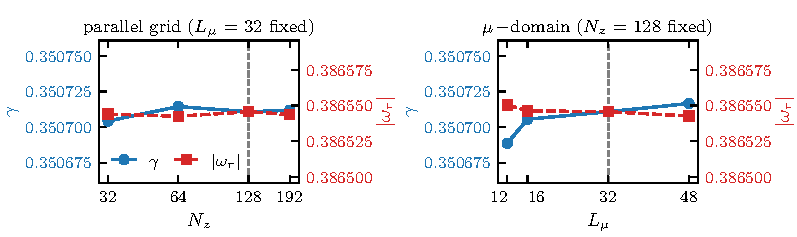
\includegraphics{plots/dipole_csurf_convergence.pdf}
\caption{Numerical-grid convergence of the dipole linear eigenvalues at $k_y\lambdaD=0.204$, $c_\mathrm{surf}=1.001$ (on the complex-pair branch past the branch collision of \Cref{fig:dipole_csurf_kyscan}). \textit{Left:} $\gamma$ (blue) and $|\omega_r|$ (red), in units of $c_s/L_\mathrm{ref}$, vs.\ the parallel-grid resolution $N_z$, with $L_\mu = 32$ held fixed. \textit{Right:} the same eigenvalues vs.\ the $\mu$-coordinate domain extent $L_\mu$, with $N_z = 128$ held fixed. Vertical dashed line: the grid $(N_z, L_\mu) = (128, 32)$ used for the $c_\mathrm{surf}$ eigenvalue scan.}
\label{fig:dipole_csurf_convergence}
\end{figure}

The trapped/passing boundary of \Cref{fig:vsp_resolution_check} (white dashed) opens as $c_\mathrm{surf}$ increases, and the dominant eigenmode migrates from a purely passing-particle response at $c_\mathrm{surf} = 1.001$ to one with substantial weight inside the trapped region at $c_\mathrm{surf} \ge 1.2$. This is the trapped-particle response described in \cref{app:dipole_lin_landscape} and visible in the off-equator parallel structure of the saturated nonlinear state (\cref{sec:dipole_phasemix}). The eigenmode decays smoothly towards the $(v_\parallel, \mu)$ box edges and shows no accumulation at the trapped/passing boundary, which indicates that the eigenvalue-scan grid $(N_{\vpar}, N_\mu, L_{\vpar}, L_\mu) = (56, 48, 3.5, 32)$ resolves the mode. The same migration appears at the $\eta = 0$ nonlinear-run drive, $\omega_n = 2$ (not shown), so the onset of trapped-particle character follows the magnetic geometry rather than the drive.

\begin{figure}
\centering
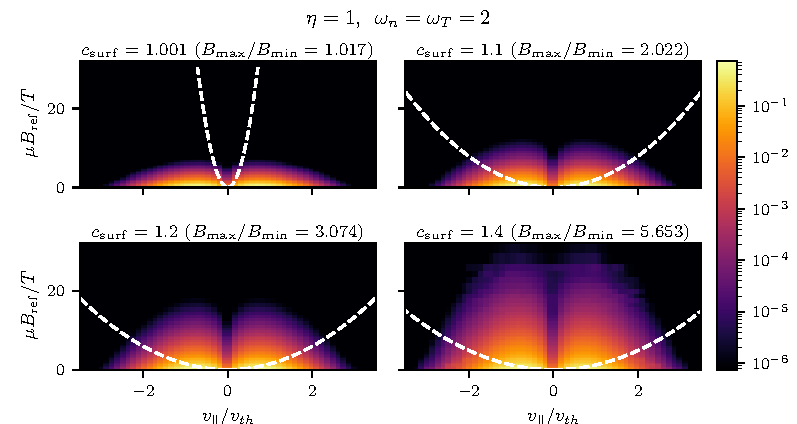
\includegraphics[width=\textwidth]{plots/appendix_vsp_resolution_check.pdf}
\caption{Velocity-space resolution check across the dipole $c_\mathrm{surf}$ scan: $|\langle f\rangle|^2$ of the dominant linear eigenmode, summed over $z$ and species, on the $(v_\parallel, \mu)$ plane at fixed $k_y\lambdaD = 0.068$ for $c_\mathrm{surf} = 1.001,\,1.10,\,1.20,\,1.40$ (panels left to right, top to bottom, with the well depth $B_\mathrm{max}/B_\mathrm{min}$ in each title), at $\eta = 1$, $\omega_n = \omega_T = 2$, on the eigenvalue-scan velocity-space grid. White dashed: the trapped/passing boundary at the $z = 0$ slice.}
\label{fig:vsp_resolution_check}
\end{figure}

The shaded bands of \Cref{fig:direct_cascade_flux} are the scatter between time segments. Over a window of that length, the scatter measures the non-stationarity of the simulation as much as the statistical uncertainty. In the $Z$-pinch, we double the radial resolution and find the level of the constant-flux $\Pi_Z$ plateau reproduced within the segment-to-segment scatter on a matched window. The doubled-resolution simulation ends before the zonal lock, so we make that check on the forming state. For the arrested transport floor of \cref{sec:saturation}, we double each velocity-space resolution separately on restarts of the production run, $N_{\vpar}$ from $64$ to $128$ and $N_\mu$ from $32$ to $64$, and compare on a matched window. Either doubling shifts the particle-flux floor by less than the floor's own slow drift between windows of the parent simulation, and leaves the heat-channel floor unchanged. In the dipole, we refine the parallel grid and find the share of the potential's parallel power in the field-line-independent (flute) component unchanged.


\section{Numerical validation of the dipole dispersion}\label{app:theory_compare}

As $c_\mathrm{surf}\to1$ the dipole module of \cref{app:dipole_impl} recovers \gene's $Z$-pinch. The metric reduces to the $Z$-pinch values term by term, to within $0.2\%$ at $c_\mathrm{surf}=1.001$ (\Cref{tab:metric_match}), and the linear dispersion $\gamma(k_y)$ reproduces \gene's $Z$-pinch dispersion to within a few parts in a hundred where the growth rate is largest. The fractional difference grows towards the band edges, where $\gamma$ is small. The dominant physical branch is recovered across the unstable band at every $c_\mathrm{surf}$ in the scan (\Cref{fig:dipole_csurf_kyscan}), and both branches at $c_\mathrm{surf} = 1.2$ (\cref{app:dipole_lin_landscape}). We now check the module away from the $Z$-pinch limit.

\citet{MPH2018} derive a bounce-averaged drift-kinetic dispersion relation for the symmetric pair plasma in dipole geometry (their equation~3.10) and solve it in the $Z$-pinch ($c_\mathrm{surf}\to1$) and point-dipole ($c_\mathrm{surf}\to\infty$) limits. We call it the bounce-harmonic (BH) dispersion and evaluate it at intermediate $c_\mathrm{surf}$, including the production value, with the $J_0^2$ finite-Larmor-radius factor retained. Specialised to a purely growing mode $\omega = \mathrm{i}\gamma$, it reads
\begin{equation}\label{eq:disp_BH}
1 + k_\perp^2 \lambdaD^2 \;=\; \frac{1}{n_0}\,\int_0^\infty\! \rmd v\,4\pi v^2 f_M(v)\,\int_0^{1/B_\mathrm{min}}\! \rmd\lambda\,\hat\tau(\lambda)\,\overline{J_0^2}(\lambda, v)\,\frac{\gamma^2 + \overline{\omega_d}(\lambda, v)\,\omega_*^T(v)}{\gamma^2 + \overline{\omega_d}^2(\lambda, v)},
\end{equation}
with $f_M(v)$ the normalised Maxwellian equilibrium, the orbit average and orbit time $\hat\tau(\lambda)$ of \cref{eq:orbit_avg} (the guiding-centre $\propto B(l)$ weight kept so the phase-space volume is correct at finite $c_\mathrm{surf}$), $\overline{\omega_d}$ the bounce-averaged magnetic drift of \cref{eq:vd}, and $\omega_*^T$ the diamagnetic frequency of \cref{eq:vstar}. It reduces to the $Z$-pinch result of \citet{MPH2018} (their equation~4.2) as $c_\mathrm{surf}\to1$, and to their point-dipole dispersion (equations~5.1--5.5) as $c_\mathrm{surf}\to\infty$, via the Kesner--Hastie deep-dipole drift $\overline{\omega_d}\to(4 k_y T/3e\psi)\,v^2$ \citep{KesnerHastie2002}. We solve the relation exactly at the simulation parameters ($c_\mathrm{surf}$, $\omega_n$, $\omega_T$, $\lambdaD$), with nothing adjustable. The only numerical content is the quadrature.

We discretise with Gauss--Laguerre quadrature in $v^2$ and a $\lambda$ grid refined across the trapping boundary $\lambda = 1/B_\mathrm{max}$. Doubling both quadrature grids moves the tabulated peaks by less than $0.3\%$. Past the branch collision, we continue the complex-pair branch into the upper-half $\omega$-plane with the argument-principle solver of \citet{IvanovAdkins2023}, avoiding the branch cuts that make such bounce-averaged continuations delicate \citep{Sugama1999, Helander2011}.

At matched wavenumber, theory and \gene\ agree at the five-per-cent level for the four values of $c_\mathrm{surf}$ at which \gene\ eigenvalues are available (\Cref{tab:BH_results}; \gene\ grid convergence in \cref{app:convergence}), and the agreement does not degrade as the well deepens. The dominant-root curves are overlaid on \Cref{fig:dipole_csurf_kyscan} for both drives. The residual deficit at the three shallowest wells is consistent with the flute closure $\phi \approx \bar\phi$ that underlies the bounce average. That closure does not resolve the eigenmode's finite $z$-envelope (\Cref{fig:dipole_lin_eigenmode_z}). The analytical dispersion is therefore a parameter-free cross-check on the dipole implementation over a range of $c_\mathrm{surf}$ that brackets the production value $1.10$ of \cref{sec:dipole}.


\begin{table}
\centering
\renewcommand{\arraystretch}{1.15}
\begin{tabular}{ccccc}
\hline
$c_\mathrm{surf}$ & BH $\gamma_\mathrm{max}$ (\ref{eq:disp_BH}) & \gene\ $\gamma_\mathrm{max}$ ($k_y\lambdaD$) & BH at that $k_y$ & relative error \\
\hline
$1.001$ & $1.36$ & $1.43$ ($0.043$) & $1.36$ & $-4.8\%$ \\
$1.01$  & $1.36$ & $1.27$ ($0.090$) & $1.20$ & $-5.0\%$ \\
$1.1$   & $1.39$ & $1.36$ ($0.073$) & $1.29$ & $-4.7\%$ \\
$1.2$   & $1.43$ & $1.30$ ($0.081$) & $1.31$ & $+1.0\%$ \\
$1.3$   & $1.48$ & ---              & ---    & ---      \\
$1.4$   & $1.53$ & ---              & ---    & ---      \\
\hline
\end{tabular}
\caption{Peak growth rate $\gamma_\mathrm{max}$ (units $10^{-2}\,c_s/L_\mathrm{ref}$) over $k_y\lambdaD \in [0.04, 0.5]$ at the six $c_\mathrm{surf}$ values, from the bounce-harmonic kinetic dispersion \cref{eq:disp_BH}, solved exactly at the simulation parameters, and from the dominant physical eigenvalues of the \gene\ scans of \Cref{fig:dipole_csurf_kyscan}. Drive $\eta = 1$ ($\omega_n = \omega_T = 2$). The relative error is quoted at matched wavenumber, the bounce-harmonic value minus the \gene\ value, normalised to the latter, with both evaluated at the $k_y\lambdaD$ of the \gene\ in-window peak (bracketed). No \gene\ eigenvalue data are available at $c_\mathrm{surf} = 1.3$ and $1.4$.}
\label{tab:BH_results}
\end{table}

\section{Dissipation and the transport floor}\label{app:epsy}

The saturation argument of \cref{sec:saturation} relies on which channels are open to the free energy rather than on the strength of the sink. This appendix demonstrates that claim with numerical experiments at fixed drive ($\eta = 0$, $\omega_n = 2$) and fixed box. Except where stated, every experiment below is a branch restarted from the arrested state of one simulation, the weakly driven production run of \cref{sec:nl_weak} carrying the velocity-space sink alone ($\varepsilon_v = 0.2$, $\varepsilon_y = 0$). We call that run the parent; its arrested flux is the floor, and every measurement below is quoted against it.

There are four key points\begin{itemize}
\item The condensate suppresses the fluctuation band without stabilising it. Reseeded fluctuations regrow exponentially in the lanes where the zonal shear passes through zero (\cref{app:epsy_regrowth}).
\item The transport-free zonal state exists but it is a fixed point and not the attractor. This state is unstable to reseeding and the floor is the level to which a condensate free to readjust relaxes (\cref{app:epsy_attractor}).
\item The level of the floor is insensitive to the strength of the velocity-space sink. We scan $\varepsilon_v$ over a factor of four at fixed drive and box and the arrested flux moves by under a tenth on matched windows. A perpendicular sink is different in kind. It acts on the transport-carrying fields directly, and scanning its coefficient over a factor of twenty with the velocity-space sink removed leaves the arrested level between about half the floor and the floor itself (\cref{app:epsy_sink}).
\item The nonlinearity moves free energy between scales but does not remove it, so in a steady state \cref{eq:W_balance} pins the injection, a gradient-weighted combination of the fluxes, to the dissipation rate. This is the conservation argument of \cref{sec:invariants} and \cref{sec:saturation} and needs no experiment. Where in wavenumber the free energy enters and leaves is measured in \cref{app:epsy_kspace}.
\end{itemize}
Two sets of runs are not branches of the parent: the strongly driven run of \cref{app:epsy_decay}, which has not reached a floor at all and which supplies the right-hand panel of \Cref{fig:permode_rates}, and the adapted-sink runs of \cref{app:epsy_gyroles}, which start from the initial condition. Together these four points give a finite floor. A state with zero transport is available but the turbulence does not stay in it.


\subsection{Suppression without stabilisation}\label{app:epsy_regrowth}

Zonally generated shear is not sufficient to stabilise the linear modes as can be seen in \Cref{fig:seeded_regrowth}. We reseed the arrested state with non-zonal fluctuations at $10^{-8}$ of their former amplitude (far too small to disturb the zonal flow). The state regrows them through some fifteen decades in energy exponentially at $\gamma_\mathrm{eff} = 0.66\,\gamma_\mathrm{lin}$ over the middle of that rise and more slowly as nonlinearity sets in (left-hand column of \Cref{fig:seeded_regrowth}). The reseeded modes grow whether the zonal condensate is frozen (right-hand column) or is allowed to evolve self-consistently (left-hand column). 

\begin{figure}
\centering
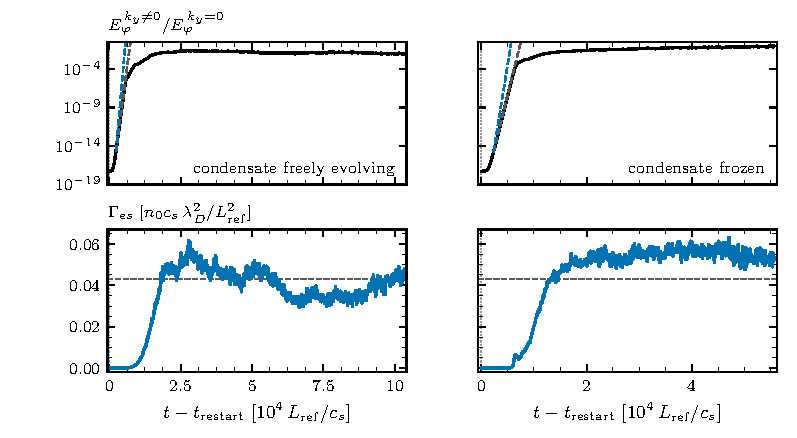
\includegraphics[width=\textwidth]{plots/seeded_regrowth.pdf}
\caption{[$\eta = 0$, $\omega_n = 2$] The locked state of the weakly driven $Z$-pinch reseeded with non-zonal fluctuations at $10^{-8}$ of their former amplitude. \textit{Left column:} the condensate freely evolving. \textit{Right column:} the condensate frozen in place. \textit{Top row:} non-zonal-to-zonal energy ratio, log scale, with dashed guides at $\gamma_\mathrm{eff}$ (grey) and $\gamma_\mathrm{lin}$ (blue) and a dotted vertical at the restart. \textit{Bottom row:} particle flux $\Gamma_{es}(t)$ of \cref{eq:flux_def}, running time-average, in mixing-length units built on $\lambdaD$; dashed, the parent's arrested floor.}
\label{fig:seeded_regrowth}
\end{figure}

The condensate's shearing rate $S(x) = \partial_x \bar v_y$ has a root mean square value of $2.6\,\gamma_\mathrm{lin}$ but passes through zero at many locations in the box. Approximately one sixth of the box lies in lanes with $|S| < \gamma_\mathrm{lin}$ in which the drive outruns the shear and it is in these lanes that the non-zonal modes are regrown. The bottom row of \Cref{fig:zonal_shear_profile} shows the zonal density, temperature and pressure corrugations of the same slice, all varying on the radial scale of the flow. The temperature and pressure corrugations are statistically indistinguishable inside and outside the lanes, and the density corrugation is only mildly weaker in them. None of the three tracks the lane pattern. The lanes are therefore a property of the shear profile and not of any corrugation in the zonal thermodynamic fields, and the corrugations are far too weak to render the interchange locally marginal, so the lanes remain linearly supercritical. The mean profiles carry no staircase: the suppression is kinematic rather than thermodynamic, and the arrest is carried by the flow alone. 

\begin{figure}
\centering
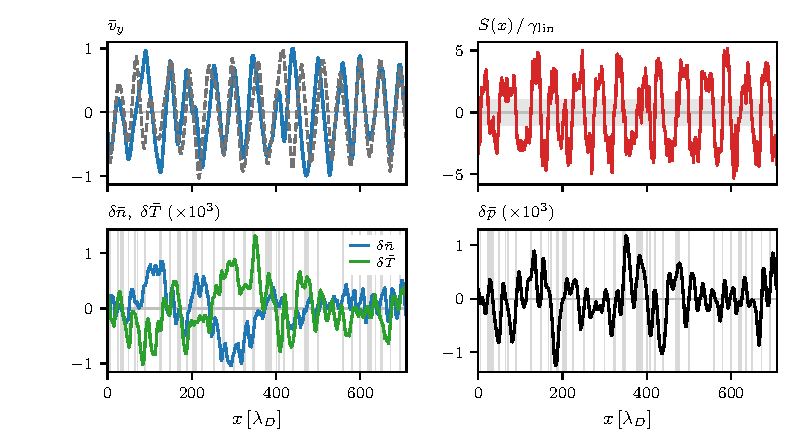
\includegraphics{plots/zonal_shear_profile.pdf}
\caption{[$\eta = 0$, $\omega_n = 2$] Real-space structure of the locked $Z$-pinch condensate, the parent state of \Cref{fig:zonal_surgery,fig:seeded_regrowth}; all four panels describe the same time slice on the same radial axis. \textit{Top left:} the zonal flow $\bar v_y(x)$ of the parent state (solid) and of the condensate rebuilt by the turbulence after the zonal modes were zeroed (dashed, \Cref{fig:zonal_surgery}), both normalised to the parent's maximum. \textit{Top right:} the parent's zonal shearing rate $S(x) = \partial_x \bar v_y$ in units of the peak linear growth rate $\gamma_\mathrm{lin}$. The shaded band marks $|S| < \gamma_\mathrm{lin}$, the lanes in which the linear drive outruns the shear. \textit{Bottom left:} the parent's zonal density and temperature corrugations $\delta \bar n$ and $\delta \bar T$, mean-subtracted. \textit{Bottom right:} the zonal pressure corrugation $\delta \bar p$, mean-subtracted. In both bottom panels the shaded vertical strips are the top right-hand panel's weak-shear lanes.}
\label{fig:zonal_shear_profile}
\end{figure}

The regrowth is localised in lanes where the zonal shear is less than the linear growth rate. Averaged over the exponential rise the non-zonal envelope stands more than thirty times higher inside them than outside. The low-shear lanes carry more than four fifths of the fluctuation energy (\Cref{fig:lane_localisation}, left-hand side). The contrast collapses back to one as the state saturates (right-hand side). The lanes are where the band grows but not where the saturated turbulence sits.

\begin{figure}
\centering
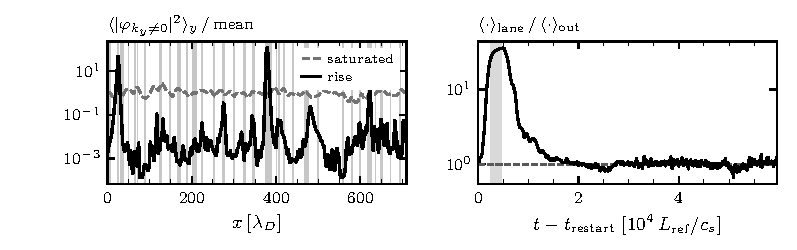
\includegraphics{plots/lane_localisation.pdf}
\caption{[$\eta = 0$, $\omega_n = 2$] Localisation of the reseeded band relative to the zero-shear lanes. \textit{Left:} the $y$-averaged non-zonal envelope $\langle|\varphi_{k_y\neq0}|^2\rangle_y(x)$, normalised to its $x$-mean, averaged over the exponential rise of \Cref{fig:seeded_regrowth} (solid) and over the saturated state (dashed); shaded, the lanes $|S| < \gamma_\mathrm{lin}$ of \Cref{fig:zonal_shear_profile}. \textit{Right:} the lane contrast, the mean envelope inside the lanes over the mean outside, per snapshot; shaded, the rise window of the left panel; dashed, no contrast.}
\label{fig:lane_localisation}
\end{figure}

\subsection{The transport-free fixed point and the attractor}\label{app:epsy_attractor}

A transport-free zonal state is a fixed point of the dynamics but the floor is the attractor. We restart the same arrested state twice, zeroing complementary halves of the spectrum (\Cref{fig:zonal_surgery}). With the non-zonal modes zeroed (left-hand column) \textcolor{red}{the zonal modes are undamped (e.g., there is no spurious numerical damping)} and the flux stays identically zero. This is the zero-transport state, and it persists for as long as nothing perturbs it: any perturbation, however small, is regrown in the regions of low shear of \cref{app:epsy_regrowth}. With the zonal modes zeroed instead (right-hand column) the turbulence rebuilds them. The flux overshoots the floor by a factor of four before settling back to within about a tenth of it, and the zonal fraction recovers to $0.92$ against the parent's $0.95$. The rebuilt condensate is drawn against its parent in \Cref{fig:zonal_shear_profile}. It recovers the parent's amplitude and band structure but not its exact profile. 

\begin{figure}
\centering
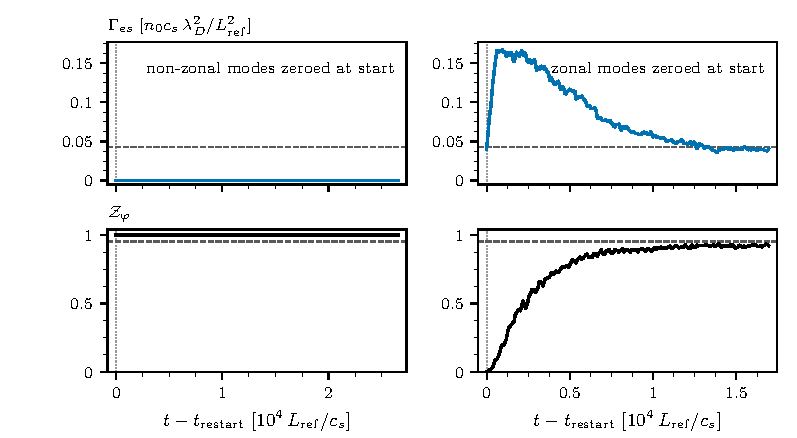
\includegraphics[width=\textwidth]{plots/zonal_surgery.pdf}
\caption{[$\eta = 0$, $\omega_n = 2$] Restart experiments on the locked state of the weakly driven $Z$-pinch: both from the same parent state at time zero, zeroing complementary halves of the spectrum. \textit{Left column:} non-zonal ($k_y \neq 0$) modes zeroed at the restart. \textit{Right column:} zonal ($k_y = 0$) modes zeroed at the restart. \textit{Top row:} particle flux $\Gamma_{es}(t)$ of \cref{eq:flux_def} in mixing-length units built on $\lambdaD$; dashed, the parent's arrested floor. \textit{Bottom row:} zonal fraction $\mathcal{Z}_\varphi(t)$ of \cref{eq:zonal_fraction}; dashed, the parent's value at restart. Running time-averages.}
\label{fig:zonal_surgery}
\end{figure}

The level of the transport floor is set by the flow's freedom to readjust. We repeat the reseeded restart with the condensate frozen so that the zonal modes reset to the parent state at every timestep (right-hand column of \Cref{fig:seeded_regrowth}). The growth rate $\gamma_\mathrm{eff}$ agrees with the free run to within $2\%$ (top row), but the frozen flow cannot readjust and admits a higher fluctuation level. Its flux settles at about $1.3$ times the parent's floor, while the freely evolving run returns to the floor itself (bottom row). We have no closed estimate of the floor's level and attempt none here.

\subsection{The strength and the structure of the sink}\label{app:epsy_sink}

If the floor is set by which channels are open rather than by the strength of the sink, two things follow. Changing that strength should barely move the floor, and changing which fields the sink acts on should move it instead, although not necessarily by much.

\textcolor{red}{We scan the velocity-space coefficient over $\varepsilon_v = 0.1$, $0.2$ and $0.4$ at fixed drive and fixed box, a factor of four in the strength of the sink. The steady-state fluxes do not change. That scan is not drawn; the two figures of this subsection carry the structure of the sink rather than its strength.}

\Cref{fig:sink_endstates} shows the end states of three different sink structures. With the velocity-space sink alone the flux arrests at the floor\textcolor{red}{, that run being the parent itself and its steady-state flux the definition of the floor}. With the perpendicular sink alone the particle flux arrests at about two thirds of the parent's floor over the interval shown, while the heat flux stays within about a tenth of the parent's heat flux. With no sink at all there is no steady state; the free energy grows steadily while the transport holds finite. That simulation is reliable only for a finite time: the drift resonance generates ever finer structure in $\vpar$, and once the true solution reaches the grid spacing the discrete solution spuriously returns free energy from the finest resolved scales to the coarsest. From that recurrence time onwards the run no longer represents a collisionless plasma, and the no-sink trace is drawn faded beyond it. \textcolor{red}{\Cref{fig:sink_endstates} draws the two fluxes alone, so the growth of the free energy in the no-sink run is not shown there.}

\begin{figure}
\centering
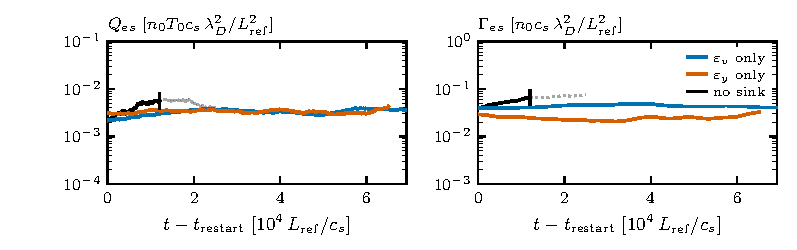
\includegraphics{plots/sink_endstates.pdf}
\caption{[$\eta = 0$, $\omega_n = 2$] Species-summed electrostatic fluxes of \cref{eq:flux_def} for the $Z$-pinch under the three dissipation structures, running time-average, log scale, in mixing-length units built on $\lambdaD$. \textit{Left:} heat flux $Q_{es}(t)$. \textit{Right:} particle flux $\Gamma_{es}(t)$. The three runs differ only in the sink: the velocity-space sink alone ($\varepsilon_v$ only), the perpendicular sink alone ($\varepsilon_y$ only), and no sink at all. In both panels the no-sink simulation is reliable only up to the velocity-grid recurrence time, marked by the short vertical bar, and is drawn faded beyond it [see text]. Time is measured from the restart of the two branch runs.}
\label{fig:sink_endstates}
\end{figure}

\Cref{fig:epsy_scan} varies the coefficient of the perpendicular sink over a factor of twenty with the velocity-space sink removed, each run restarted from the arrested state of the parent. Every trace arrests, and the arrested particle flux lands between $0.45$ and $0.96$ of the parent's floor across the full range of the coefficient, with no monotonic dependence on it. The electrostatic energy climbs slowly in every branch: the perpendicular sink spares the zonal modes, so nothing removes $E$ from the condensate and it keeps charging at the rate the inverse transfer delivers (\cref{sec:direct_cascade_flux}).

\begin{figure}
\centering
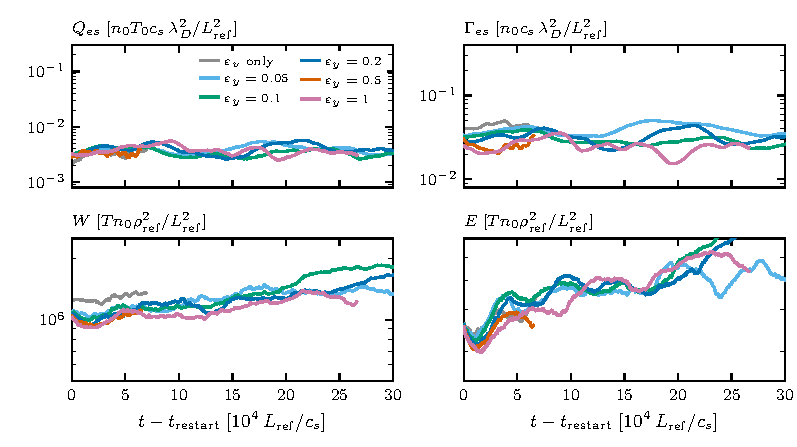
\includegraphics{plots/epsy_scan.pdf}
\caption{[$\eta = 0$, $\omega_n = 2$] The perpendicular-sink-only runs ($\varepsilon_v = 0$) at five values of the coefficient $\varepsilon_y$, each restarted from the arrested state of the $\varepsilon_v$-only run (grey). \textit{Top row:} species-summed heat and particle fluxes of \cref{eq:flux_def}, running time-averages, in mixing-length units built on $\lambdaD$. \textit{Bottom row:} the free energy $W$ and the electrostatic energy $E$. All panels log scale; time is measured from the restart. The axis is truncated at $3\times10^{5}$ and the three longest simulations continue past it, the arrested levels quoted in the text being read at the end of each record. The five coefficients are $\varepsilon_y = 0.05$, $0.1$, $0.2$, $0.5$ and $1$.}
\label{fig:epsy_scan}
\end{figure}


\subsection{Where the free energy enters and where it leaves}\label{app:epsy_kspace}


\Cref{fig:permode_rates} resolves the budget of \cref{eq:rev_irr} by mode, along $k_x$ at the smallest finite $k_y$, as rates per unit mode energy averaged over a late window of each simulation. The drive is confined to long radial wavelength and is not of one sign, two fifths of the radial modes at this $k_y$ carrying a net negative drive, but the negative modes sum to a small fraction of the positive ones, so summing the signed drive over $k_x$ costs little. The eigenmode pairing of \cref{sec:linear} leads one to expect as much, a damped root of equal magnitude accompanying each unstable one and returning free energy to the gradient rather than destroying it. The removal rate of the velocity-space sink instead grows monotonically along $k_x$. The zonal advection conserves $k_y$ and sweeps only $k_x$, so the sweep carries every fluctuation towards stronger removal, whatever the sink coefficient. The growth of the removal along $k_x$ is inherited rather than intrinsic, since the sink is a pure $\vpar$ operator \cref{eq:hypv_charge} and the modes the sweep has carried furthest are those the drift resonance has phase-mixed for longest. \textcolor{red}{This is in contrast to a cascade of the Kolmogorov kind, whereby the energy is imagined to reach the dissipation scale in one turnover time of the outer scale, owing to the acceleration of the nonlinear turnover rate with wavenumber. The key difference here is that the zonal shearing does not act this way: under a steady shear the radial wavenumber of a fluctuation increases linearly in time, so the velocity-space structure develops secularly over the $k_x$ sweep, and the drift resonance, whose rate is set by $k_y$ alone, has more time to act the further along $k_x$ a fluctuation has been carried.} The right-hand panel repeats the measurement for the strongly driven run, where the drive sits two orders of magnitude below the removal: over the drainage the sink dominates every mode's budget.

\begin{figure}
\centering
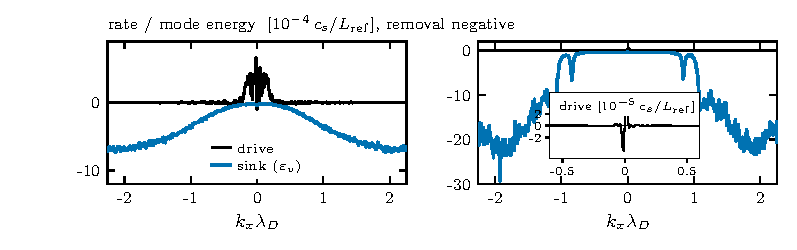
\includegraphics{plots/permode_rates.pdf}
\caption{[$\eta = 0$ and $\eta = 1$, $\omega_n = 2$] Per-mode drive and sink rates, each divided by the free energy of the same mode, against $k_x\lambdaD$ at the lowest finite $k_y$ (the same mode in both panels, which share a box). The drive is the diamagnetic injection $T_W^\mathrm{drive}$ of \cref{eq:rev_irr}, the only linear source of free energy, the magnetic-drift term cancelling between $W$ and $E$ and the nonlinearity conserving $W$; the sink is the dissipative channel $T_W^\mathrm{diss}$, which in every run shown is the velocity-space hyperdiffusion $\varepsilon_v$ of \cref{eq:hypv_charge} acting alone. Both rates are time-averages over a late-time window of each simulation, so every curve is an effective per-mode rate rather than an instantaneous one. Injection is positive and removal negative, with a dotted line at zero; note the differing vertical ranges. \textit{Left:} the weakly driven run, over its arrested flux-floor window. \textit{Right:} the strongly driven run, over its late flux oscillation. The inset shows this panel's drive at its own scale, two orders of magnitude below its removal.}
\label{fig:permode_rates}
\end{figure}

\Cref{fig:drive_vs_gamma} sets the drive against the linear growth rate of the same $k_y$, for both runs. A fluctuation made of the unstable eigenmode alone would draw free energy at exactly $2\gamma_\mathrm{lin}$, since $W$ grows at twice the mode rate. \textcolor{red}{Two drive rates are compared with it, the net and the gross,}
\begin{equation}\label{eq:gross_net}
\textcolor{red}{\sum_{k_x}\bigl\langle T_W^\mathrm{drive}(\vec k)\bigr\rangle \quad\text{(net)}, \qquad \sum_{k_x}\bigl\langle\bigl|T_W^\mathrm{drive}(\vec k)\bigr|\bigr\rangle \quad\text{(gross)},}
\end{equation}
\textcolor{red}{each divided by the free energy of the same $k_y$, where $\langle\cdot\rangle$ is the time average over the window. A mode that draws free energy from the gradients and later returns it contributes to the gross rate but not to the net.} At $\eta = 0$ (left-hand side) the measured net injection is about a fifth of $2\gamma_\mathrm{lin}$ over most of the band, rising steeply near the upper band edge as the linear growth rate goes to zero, while the gross rate runs from about two thirds of $2\gamma_\mathrm{lin}$ at the longest wavelength to a quarter of it near the linear peak. The give and take is therefore real, and largest at the largest scale, where the gross rate is three times the net. Near the linear peak most of the shortfall is instead that the fluctuation is not the unstable eigenmode. In neither case is the shortfall a near-cancellation of two large opposing terms. {\color{red}At $\eta = 1$ (right-hand side) both rates lie orders of magnitude below $2\gamma_\mathrm{lin}$, the gross at a hundredth of it at most and the net some three hundred times smaller again, so that the exchange with the gradients is almost all give and take and what it leaves is a part in ten thousand of what the sink removes. There the shortfall is a near-cancellation, and the transport carries the same residue: the residual flux of \cref{sec:nl_eta1} is what that cancellation leaves in the heat and particle channels. The net is drawn solid where its window mean clears twice its own sampling noise, which is two thirds of the unstable modes, and dotted elsewhere.

The channels themselves are drawn in \Cref{fig:budget_rates}. At $\eta = 0$ the injection is confined to $k_y\lambdaD \lesssim 1$, the removal rises monotonically through the band and overtakes the drive near $k_y\lambdaD \approx 1$, where the linear growth rate changes sign, and the transfer follows the difference between the drive and the removal, exporting free energy from every wavenumber below the crossing and delivering it to every wavenumber above. The three channels balance at each $k_y$ to a median residual under a tenth of the largest of them.} The exchange between growing and damped modes therefore runs alongside the cascade rather than replacing it. Transfer between $k_y$ bands is carried by triads of non-zonal modes alone, and on either route the free energy is erased only when the drift resonance has delivered it to fine $\vpar$ structure. The zonal modes stand apart: they carry rather more than half of the free energy and four fifths of the electrostatic energy, take none of the drive, and exchange with the rest of the spectrum at a net rate of about a hundredth of the injection, so that their turnover time exceeds the length of the simulation.

\begin{figure}
\centering
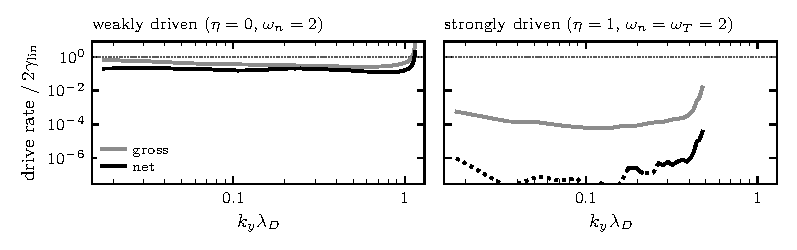
\includegraphics{plots/drive_vs_gamma.pdf}
\caption{\textcolor{red}{The drive against the linear growth rate at each $k_y$, over each run's linearly unstable range: the net drive of \cref{eq:gross_net}, which counts the exchange with the gradients with its sign, and the gross drive, which counts every gain and every loss without regard to sign, each divided by the free energy of the same $k_y$, time-averaged, and drawn as a fraction of $2\gamma_\mathrm{lin}(k_y)$. \textit{Left-hand side:} the weakly driven baseline, over the arrested floor. \textit{Right-hand side:} above the fluid threshold, over the drainage. The gap between the two curves is the exchange that never reaches the sink. The net is drawn solid where its window mean clears twice its own sampling noise and dotted elsewhere. Dotted, unity, where the drive matches the linear rate. Both axes logarithmic.}}
\label{fig:drive_vs_gamma}
\end{figure}

\subsection{The free decay of the strongly driven store}\label{app:epsy_decay}

In \cref{sec:rev_irr} two claims are made about the strongly driven $\eta = 1$ run, both are measured here: that its store of free energy is draining and draining more slowly as it empties, and that the two channels of its injection come nowhere near cancelling, so a steady state still needs the sink. The decay is the falling black trace in the right-hand column of \Cref{fig:flux_timeseries}; the weakly driven runs of \Cref{fig:epsy_scan} are not draining, their free energy holding steady or drifting slowly upward.

Take the drain first. Suppose the turbulence disposes of free energy at a single rate set by the fluctuation amplitude itself,
\begin{equation}\label{eq:app_epsy_rate}
\tau^{-1} \;\propto\; W^{1/2} ,
\end{equation}
as is the case in freely decaying two-dimensional turbulence \citep{Batchelor1969}. Then $\rmd W/\rmd t = -W/\tau$ becomes the free-decay law
\begin{equation}\label{eq:app_epsy_decay}
\frac{\rmd W}{\rmd t} \;=\; -\,a\,W^{3/2} ,
\end{equation}
from which both properties follow. Integrating gives
\begin{equation}\label{eq:app_epsy_integrated}
W^{-1/2}(t) \;=\; W^{-1/2}(0) \;+\; \tfrac{1}{2}\,a\,t
\qquad\Longrightarrow\qquad
W \;\propto\; t^{-2}
\end{equation}
at late times, so the store empties as a power law. Dividing $W$ by its own rate of change gives the drain time at the rate it is running,
\begin{equation}\label{eq:app_epsy_tau}
\frac{W}{|\rmd W/\rmd t|} \;=\; \frac{1}{a\,W^{1/2}} \;\propto\; W^{-1/2} ,
\end{equation}
which lengthens as the store falls, so the relaxation is still running at the end of the simulation rather than having finished. This scaling has been checked in the simulation. From $t = 6\times10^{3}$ to the end of the simulation, $W^{-1/2}$ is linear in time to a relative residual of about $2\%$ in $W$.

\textcolor{red}{The same law can be used to approximate how far the run is from a steady state, and how long it would take to get there. The store stops falling when the turbulence disposes of free energy no faster than the gradients supply it, $a\,W_\infty^{3/2} = \mathcal{R}_Z + \mathcal{R}_E$, which fixes the store a steady state would hold. Over the second half of the simulation $a$ is constant to within three per cent and the injection to within a quarter, and together they put the last value of $W$ some five hundred times above $W_\infty$: the run has fallen six orders of magnitude from the burst and has nearly three more to go. Integrating \cref{eq:app_epsy_decay} from the end of the simulation down to $W_\infty$ takes about $1.4\times10^{6}$ time units, some twenty times the length of the simulation, and the power law puts three quarters of that time in the last factor of ten. Both numbers hold only while the disposal coefficient and the injection stay as they are measured now.}

The correspondence goes further than the decay rate. Over the same interval the electrostatic energy falls by about $30\%$ while $Z$ falls more than sixtyfold, so the invariant of the inverse cascade is nearly conserved while the invariant of the forward cascade decays, exactly as energy and enstrophy behave in two-dimensional free decay. Here there is a mechanism for that correspondence: the sink of \cref{eq:hypv_charge} drains $Z$ but cannot remove $E$ at all.

The injection of \cref{eq:W_balance} at $\eta = 1$ is nowhere near cancelling: over the drainage window the inward particle channel offsets between $6\%$ and $10\%$ of what the conducted heat channel injects, depending on the window. The injection therefore stays positive, and a steady state still needs the sink. \textcolor{red}{The decay phase does not end at zero. The free-decay law \cref{eq:app_epsy_decay} omits the injection, which is negligible while the dissipation dominates; with it restored, the store empties only until the dissipation has fallen to the level of the injection, and the true asymptotic state then has a $Z$-dissipation floor and a transport floor, as the $\eta = 0$ run already does [\Cref{fig:energy_balance_vs_drive}, left-hand column]. At the end of the simulation the dissipation still exceeds the mean injection by four orders of magnitude (\cref{sec:rev_irr}), so that state lies far beyond the simulation.}

\subsection{A dynamically adapted perpendicular sink}\label{app:epsy_gyroles}

The perpendicular coefficient need not be fixed by hand. The gyrokinetic large-eddy procedure of \citet{Morel2011} adapts the perpendicular dissipation dynamically to the free energy arriving at the small scales. \Cref{fig:gyroles} repeats the weakly driven run from its initial condition with this model in place of the fixed coefficient, once retaining the velocity-space sink and once with it removed. Both pass through the saturation history of the production run. The run retaining the velocity-space sink arrests at $0.78$ of the parent's floor, inside the band of \Cref{fig:epsy_scan}; the run with the dynamic model as the sole dissipation arrests lower, at $0.33$, below that band. Both ratios are read at the end of the common interval of \Cref{fig:gyroles}. The coefficient the model settles on is of order $3\times10^{-3}$, more than an order of magnitude below the smallest fixed $\varepsilon_y$ scanned there.

\begin{figure}
\centering
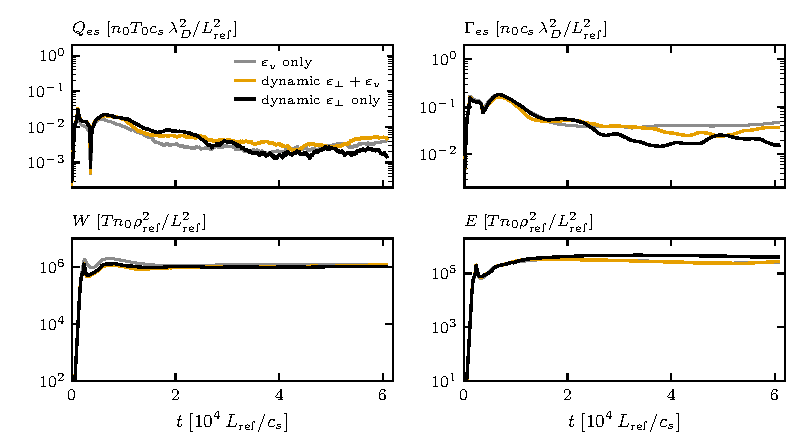
\includegraphics{plots/gyroles.pdf}
\caption{[$\eta = 0$, $\omega_n = 2$] The production run ($\varepsilon_v$ only, grey) against two runs with the perpendicular dissipation adapted dynamically, one retaining the velocity-space sink and one without it, all started from the same initial condition. \textit{Top row:} species-summed heat and particle fluxes of \cref{eq:flux_def}, running time-averages, in mixing-length units built on $\lambdaD$. \textit{Bottom row:} the free energy $W$ and the electrostatic energy $E$. All panels log scale; every trace is drawn over the same interval, the length of the shortest simulation.}
\label{fig:gyroles}
\end{figure}

\section{Dependence on the box aspect ratio}\label{app:aspect}

All the production runs of this paper, $Z$-pinch and dipole alike, use a radially elongated perpendicular box that is twice as long in $x$ as in $y$ on the same number of radial points so that $k_{x,\mathrm{min}} = k_{y,\mathrm{min}}/2$ and $k_{x,\max}$ is half its square-box value (\Cref{tab:setup}). The radial range given up at the fine end carries almost nothing. In the locked state of the elongated dipole run discussed below, the non-zonal energy above $k_x\lambdaD = 2$ is $3\times10^{-8}$ of the total against $5\times10^{-8}$ above the same wavenumber in the square box. We choose the extra radial length for the following reasons. The zonal condensate occupies the longest radial mode the box admits and so the box scale constrains it. It has also been observed that the secondary instability that breaks up the streamers can require perturbations with $k_x < k_y$ \citep{ClarkeUnpub} and so the box must also carry modes long enough in $x$ to break its own longest streamer. Elongating in $x$ supplies both and is standard in strongly driven gyrokinetic simulations \citep{Jenko2000, Rogers2000}.

\Cref{fig:dipole_morph_aspect} compares the $\eta = 1$ dipole run (right-hand column) with the equivalent run in a square box (left-hand column, $k_{x,\mathrm{min}} = k_{y,\mathrm{min}}$). The stages are the same in both: streamers form, steepen and break, and the same zonal-locked state emerges. The condensate occupies the longest radial mode each box admits and about $99\%$ of the zonal energy moves to the new box scale when $k_{x,\mathrm{min}}$ halves. \citet{ClarkeUnpub} observe the same box-scale selection across an aspect-ratio scan reaching $L_x = 12 L_y$.

The widening does not weaken the zonal shear. The peak shearing rate, measured on the equatorial zonal profile at matched times after each lock, is about $40\%$ higher in the elongated box than in the square one on bands twice as wide. Both rates are more than fifty times the linear growth rate. The condensate amplitude grows as $k_{x,\mathrm{min}}$ falls so halving $k_{x,\mathrm{min}}$ maintains the shear rather than diluting it \citep{Waltz1994, ClarkeUnpub}.

The boxes differ at late times (bottom row). The square-box zonal state has broken up. Its bands have given way to a box-scale structure extended in $x$ and its zonal fraction has fallen below $0.1$. The elongated box retains its condensate to the latest time reached which is about four times the breakup time of the square-box state. Its zonal fraction is still near unity. 

\begin{figure}
\centering
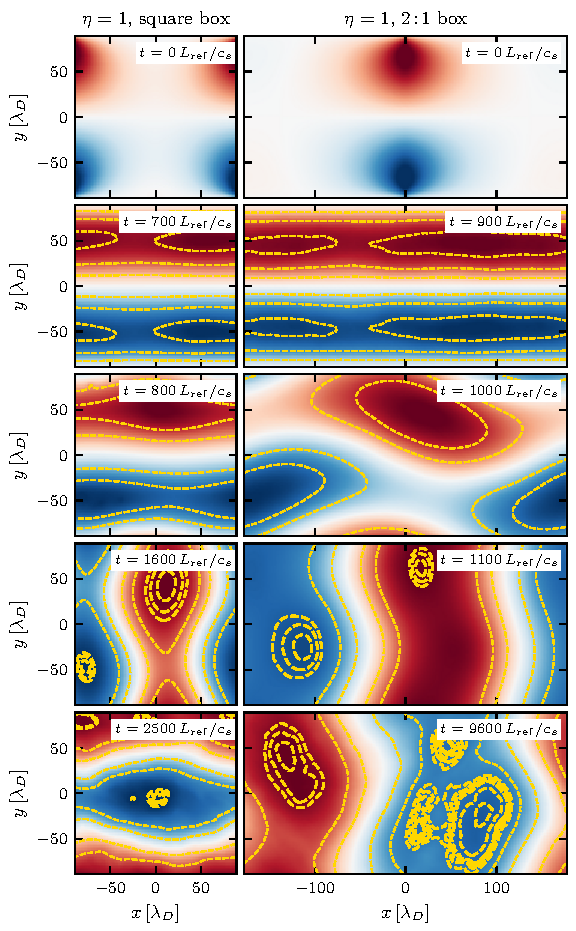
\includegraphics{plots/dipole_morph_aspect.pdf}
\caption{As \Cref{fig:dipole_morph}, for the $\eta = 1$, $\omega_n = \omega_T = 2$ dipole drive, at the same spatial scale. \textit{Left column:} the square box ($1\!:\!1$ in $x\!:\!y$). \textit{Right column:} the radially elongated box ($2\!:\!1$). \textit{Bottom row:} the late-time state of each run. Colour scales saturate at the 99th percentile of each panel, and gold dashed contours are drawn on both columns, as in \Cref{fig:dipole_morph}.}
\label{fig:dipole_morph_aspect}
\end{figure}

\FloatBarrier

\bibliographystyle{jpp}
\bibliography{references}

\end{document}
